%#!platex manual; latexml --noparse --destination=./manual.xml manual.tex; latexmlpost --format=xhtml --destination=/home/ohori/work/WWW/pllab-www/smlsharp/docs/1.0/ja/manual.xhtml --split  --novalidate manual.xml
\documentclass{jbook}
\ifx\jp%>>>>>>>>>>>>>>>>>>>>>>>>>>>>>>>>>>>>>>>>>>>>>>>>>>>>>>>>>>>>>>>>>
\else%%%%%%%%%%%%%%%%%%%%%%%%%%%%%%%%%%%%%%%%%%%%%%%%%%%%%%%%%%%%%%%%%%%%
\fi%%%%<<<<<<<<<<<<<<<<<<<<<<<<<<<<<<<<<<<<<<<<<<<<<<<<<<<<<<<<<<<<<<<<<<
\usepackage{a4}
\usepackage{latexsym}
\usepackage{url}
\usepackage{epsfig}
\oddsidemargin 0in
\evensidemargin 0in

%%%%% 日本語
% \newcommand{\jp}{a}
% \newcommand{\txt}[2]{#1}
%%%%% 英語
\newcommand{\txt}[2]{#2}


\renewcommand{\today}{\txt{平成24年4月18日}{April 18, 2012}}
\date{\today}
\newcommand{\smlsharp}{SML\#}

\newcommand{\version}{1.0.0}
\newcommand{\smlsharpSize}{\txt{30万}{0.3 millions}}
\newcommand{\authors}
{\txt{大堀\ \ 淳\mbox{\ \ \ \ }上野 雄大}
{Atsushi Ohori\mbox{\ \ \ \ }Katsuhiro Ueno}
}

\newcommand{\func}{\rightarrow}
\newcommand{\vbar}{\mbox{\ |\ }}
\newcommand{\code}[1]{\mbox{{\tt #1}}}
\newcommand{\nonterm}[1]{\mbox{$\langle$}{\it #1}\mbox{$\rangle$}}
\newcommand{\sep}{\mbox{\ \ }}

\newenvironment{program}{\begin{tt}\begin{quote}}{\end{quote}\end{tt}}
% \newcommand{\myem}{\ \ \ \ \ \ \ }
\newcommand{\myem}{\ \ \ \ \  }
\newcommand{\myfm}{ \ \ \ \ \ }


\title{\txt{プログラミング言語\smlsharp{}解説}{\smlsharp{} Document}}
\author{
\authors
\\
\txt{東北大学 電気通信研究所}{RIEC, Tohoku University}
}

\begin{document}

\maketitle

\frontmatter
\ifx\jp%>>>>>>>>>>>>>>>>>>>>>>>>>>>>>>>>>>>>>>>>>>>>>>>>>>>>>>>>>>>>>>>>>
{\bf FireFox}などのMathMLを表示可能なブラウザでご覧ください.
\else%%%%%%%%%%%%%%%%%%%%%%%%%%%%%%%%%%%%%%%%%%%%%%%%%%%%%%%%%%%%%%%%%%%%
This document is best viewed with a MathML-capable browser such as {\bf FireFox}.
\fi%%%%<<<<<<<<<<<<<<<<<<<<<<<<<<<<<<<<<<<<<<<<<<<<<<<<<<<<<<<<<<<<<<<<<<

\chapter*{\txt{はじめに}{Preface}}

\ifx\jp%>>>>>>>>>>>>>>>>>>>>>>>>>>>>>>>>>>>>>>>>>>>>>>>>>>>>>>>>>>>>>>>>>
	本書は東北大学電気通信研究所で開発された関数型プログラミング言語
\smlsharp{}の公式ドキュメントです.
	\smlsharp{}の概要,プログラミングチュートリアル,参照マニュアル,
ツールなどの情報を含む総合ドキュメントを意図しています.
	関数型言語に慣れた人はもちろんこれからプログラミングを始めようと
する人も,\smlsharp{}言語を使って高度なプログラミングを書き始めるために
十分な情報を提供します.
	特に,第\ref{part:tutorial}部のチュートリアルは,関数型言語の基
本的な考え方やMLプログラミングの基礎を含んでおり,ML言語の手軽な教科書と
しても使用できます.
	ML言語をより本格的に学ぶには,Standard MLの教科書
\cite{ohori00sml}をご参照ください.
  
	\smlsharp{}は,これら教科書で書かれたStandard MLと後方互換性のあ
る言語です.
	ネイティブコードコンパイラですが,対話型プログラミングもサポート
しており,だれでも手軽にMLプログラミングを楽しむことができます.
	さらに,\smlsharp{}が実現しているC言語とのシームレスな連携などの
機能は,高度で信頼性の要求される本格的な実用的システムの開発にも威力を
発揮すると信じています. 
  
	本ドキュメントを参考に,\smlsharp{}プログラミングをお楽しみくだ
さい. 
	不明な点や要望等は著者にご連絡ください.
\else%%%%%%%%%%%%%%%%%%%%%%%%%%%%%%%%%%%%%%%%%%%%%%%%%%%%%%%%%%%%%%%%%%%%
	This is the official document of \smlsharp{}, a programming
language developed at Research Institute of Electrical Communication,
Tohoku University.
	This document intends to provide comprehensive information on
\smlsharp{}, covering a user's guide, tutorials on ML and \smlsharp{}
programming, and a reference manual.
	This \version{} version only contains an overview of \smlsharp{}
and tutorials on ML and \smlsharp{} programming, which would be
sufficient both for beginners who want to start writing ML programs and
for experienced ML programmer who would like to try out or switch to
\smlsharp{}.

	Send comments and questions to the authors.
\fi%%%%<<<<<<<<<<<<<<<<<<<<<<<<<<<<<<<<<<<<<<<<<<<<<<<<<<<<<<<<<<<<<<<<<<

\begin{flushright}
\txt{
2012年4月\\
東北大学電気通信研究所\\
\authors
}
{
April, 2012\\
RIEC, Tohoku University\\
\authors
}
\end{flushright}

\chapter*{\txt{本書の使い方}{How to read}}

\ifx\jp%>>>>>>>>>>>>>>>>>>>>>>>>>>>>>>>>>>>>>>>>>>>>>>>>>>>>>>>>>>>>>>>>>
    この文書の第\ref{part:outline}部の概要と第\ref{part:tutorial}部のチュー
トリアルはMLプログラミングの基礎から\smlsharp{}が提供する高度の機能まで
を習得できる構造になっています.
	先頭から順に一気にお読みになることをおすすめします.
	お急ぎの方は,以下のページにお探しの情報があるかもしれません.
\begin{description}
\item[\smlsharp{}の名前について]
第\ref{sec:smlsharpHistory}節 \smlsharp{}の歴史
\item[インストール]
第\ref{sec:tutorialInstall}節 \smlsharp{}コンパイラのインストール
\item[コマンドパラメタ]
第\ref{sec:tutorialSmlsharpParameter}節 {\tt smlsharp}コマンドの起動モード
\item[コンタクト]
第\ref{sec:smlsharpTeam}節 \smlsharp{}開発チームと連絡先情報
\item[\smlsharp{}ホームページ] 
\url{http://www.pllab.riec.tohoku.ac.jp/smlsharp/ja/}
\end{description}    

本書に関して,以下の点をご了承ください.
\begin{itemize}
\item 
	現在の第\version{}版のドキュメントはまだ未完成のドラフトです.
	特に,参照マニュアルは含まれず,MLプログラミングのチュートリ
アルも一部未完成です.

\item 随時頻繁に修正を行います.
	そのため,本文書の配布は当面xhtml形式のみとします.
	近い将来,より完成した版のPDFでの配布を検討中です.

	修正・執筆にあたっては,twitterなどでの\smlsharp{}や本書へのコメントな
ども,本書の改善の参考にさせて頂いております.
	個々に言及いたしませんが,本書をご覧頂きコメントなどの発言され
た方々に感謝いたします. 

\item この文書は,LaTeXとLaTeXMLを用いて作成しています.
FirefoxなどのMathMLのレンダリングが可能なブラウザでご覧ください.

\item LaTeXMLは日本語化がなされていないようです.
	本文書は{\tt jbook}クラスで書いていますが,LateXMLのpackageに
jbook用が用意されていないため,{\tt book.cls.ltxml}を
{\tt jbook.cls.ltxml}にコピーし使用しています.
	(LateXMLの日本語クラスパッケージをご存知の方はお教えください.)
\end{itemize}
\else%%%%%%%%%%%%%%%%%%%%%%%%%%%%%%%%%%%%%%%%%%%%%%%%%%%%%%%%%%%%%%%%%%%%

	The tutorials in parts~\ref{part:outline} and
\ref{part:tutorial} are structured in such a way that the reader can
learn from ML programming basics to advanced programming features
provided by \smlsharp{}.
	We recommend to read through these parts quickly in the order
they are presented.

	If you are in a harry, you may find the desired information in
one of the following pages.
\begin{itemize}
\item Section \ref{sec:tutorialInstall}: How to install \smlsharp{}.
\item Section \ref{sec:tutorialSmlsharpParameter}: {\tt smlsharp} command parameters.
\item Section \ref{sec:smlsharpTeam}: \smlsharp{} development team and
contact information.
\item Section \ref{sec:smlsharpHistory}: On the name of \smlsharp{}
(History of \smlsharp).
\item \smlsharp{} web page:
\url{http://www.pllab.riec.tohoku.ac.jp/smlsharp/ja/}
\end{itemize}

Please note the following.
\begin{itemize}
\item 
	This \version{} version is an incomplete draft;
it does not contain the reference manual and some part of the ML
programming tutorial is incomplete.

\item 
	This document is frequently revised and updated.
	For this reason, currently, this is only distributed on this web
server.
	In near future, we plan to include a more complete version of
this document in PDF format with \smlsharp{} distribution.

\item 
	This document is written in LaTeX and processed with LaTeXML.
	It is best viewed with a MathML-capable browser such as {\bf Firefox}.
\end{itemize}
\fi%%%%<<<<<<<<<<<<<<<<<<<<<<<<<<<<<<<<<<<<<<<<<<<<<<<<<<<<<<<<<<<<<<<<<<

\chapter*{\txt{\smlsharp{}使用上の注意}{Important notes on \smlsharp{}}}

\ifx\jp%>>>>>>>>>>>>>>>>>>>>>>>>>>>>>>>>>>>>>>>>>>>>>>>>>>>>>>>>>>>>>>>>>

\smlsharp{}\version{}版を使用する上で注意すべき点を列挙します.
\begin{enumerate}
\item  {\tt OS.FileSys.tmpName : unit -> string}関数について.\\
	基本ライブラリ(Standard ML Basis Library)で提供されているこの
関数の\version{}版での実装は,Cの標準ライブラリ関数{\tt tmpnam}を使用し
ています.
	このCライブラリ関数の使用に関しては,セキュリティ上の問題がある
ことが知られています(詳しくはBSD系のManページなどをご覧ください).
	\smlsharp{}コンパイラを使うユーザが,この基本ライブラリ関数
{\tt OS.FileSys.tmpName}を使用し一時ファイルを作成するプログラムを書いた
場合にも,同様の問題が発生する可能性があります.
  
    {\tt \_require "basis.smi"}などの宣言を通じてこの関数をリンクする実
行形式プログラムの作成時には,
\begin{program}
xxxx.o : In function `F45xxx':\\
(xxxx) : warning: the use of `tmpnam' is dangerous, better use `mkstemp'
\end{program}      
とのメッセージが出力されます.
	この警告は,この{\tt tmpnam}がリンクされていることによるものです.
  
	Cのライブラリ関数{\tt tmpnam}を使って一時ファイルを作成する上でのセ
キュリティ上の問題の一つは,一時ファイル名の生成と実際に使用する一時ファ
イルを作成する操作が分離されているために起こります.
	基本ライブラリの{\tt OS\_FILE\_SYS}シグネチャが要求する{\tt
tmpName : unit -> string}の型をもつ関数の実装を変更するのみでは,
この問題の根本的な解決は難しいと思われます.
	\smlsharp{}では,{\tt OS.FileSys}基本ライブラリモジュールに代わ
る,より安全でかつ効率と使用勝手のよいモジュールを提供することを検討中で
す.
\end{enumerate}
\else%%%%%%%%%%%%%%%%%%%%%%%%%%%%%%%%%%%%%%%%%%%%%%%%%%%%%%%%%%%%%%%%%%%%

Here, we list the issues you should aware of in using \smlsharp{}
version~\version{}.
\begin{enumerate}
\item  {\bf On the function {\tt OS.FileSys.tmpName : unit -> string}}\\
	This is a function in the Standard ML Basis Library.
	The implementation in the \version{} version uses C library
function {\bf\tt tmpnam}.
	It is know that usage of this C function has a security problem.
	(See, for example, a man page in a BSD-family OS.)
	If one write an \smlsharp{} program that manipulates
temporary files using {\tt OS.FileSys.tmpName}, the program may subject
to the same security problem.
  
	When the \smlsharp{} compiler generates an executable program
of a source program that references this function, typically through
{\tt \_require "basis.smi"} declaration, the following warning message
is printed:
\begin{program}
???.o : In function `F45???':\\
(????) : warning: the use of `tmpnam' is dangerous, better use `mkstemp'
\end{program}      
	This is due to the fact that {\tt tmpnam} is linked to the
executable program.
  
	One of the causes of the security problem in creating a
temporary file using C function {\tt tmpnam} is the separation 
of the temporary name creation and the creation of the file that is
actually used.
	We find it rather difficult to solve this problem by changing 
implementation of the function {\tt tmpName : unit -> string}, whose
signature is required by {\tt OS\_FILE\_SYS}.
	We plan to develop a new structure that would serve
a secure, efficient and usable alternative to {\tt OS.FileSys}.
\end{enumerate}
\fi%%%%<<<<<<<<<<<<<<<<<<<<<<<<<<<<<<<<<<<<<<<<<<<<<<<<<<<<<<<<<<<<<<<<<<

\tableofcontents
\mainmatter

\part{\txt{概要}{Overview}}
\label{part:outline}

\chapter{\txt{\smlsharp{}の概要}{Overview of \smlsharp{}}}
\label{chap:intro}

\ifx\jp%>>>>>>>>>>>>>>>>>>>>>>>>>>>>>>>>>>>>>>>>>>>>>>>>>>>>>>>>>>>>>>>>>
本章では\smlsharp{}言語の概要を説明します.
\else%%%%%%%%%%%%%%%%%%%%%%%%%%%%%%%%%%%%%%%%%%%%%%%%%%%%%%%%%%%%%%%%%%%%
This chapter outline the \smlsharp{} language.
\fi%%%%<<<<<<<<<<<<<<<<<<<<<<<<<<<<<<<<<<<<<<<<<<<<<<<<<<<<<<<<<<<<<<<<<<

\section{\txt{\smlsharp{}とは?}{What is \smlsharp{}?}}
\label{sec:whatIsSmlsharp}

\ifx\jp%>>>>>>>>>>>>>>>>>>>>>>>>>>>>>>>>>>>>>>>>>>>>>>>>>>>>>>>>>>>>>>>>>
\smlsharp{}は,以下のような特徴をもったML系関数型プログラミング言語です.
\begin{enumerate}
\item {\bf Standard MLとの後方互換性.}
	\smlsharp{}は,ML系言語の標準の厳密な仕様であるStandard MLとの完
全な後方互換性をもっています.
	Standard MLの形式的な仕様\cite{sml}を満たすすべてのプログラムを
コンパイルできます.

\item {\bf レコード多相性.}
	レコード多相性\cite{ohor95toplas}は,オブジェクトやデータベース
のタプルなどに現れるラベル付きレコードをML言語に完全に統合するために必要
な型システムの機能です.
	\smlsharp{}は,この機能を完全にサポートしています.

\item {\bf SQLのシームレスな統合.}
	SQLはデータベースの標準問い合わせ言語であり,データベースを利用
するプログラムで必ず必要となる機能です.
	\smlsharp{}は,SQLの一部の機能をライブラリとして提供するのでは
なく,SQLそのものを多相型をもつ第一級の式として統合しています.
	この機能により,複雑なプログラムデータベース操作を,MLプログラム
の中で直接プログラムすることができます.
	
\item {\bf C言語との直接連携.}
	システムプログラミングを含む種々のOSの機能の利用にはC言語で記述
されたライブラリへのアクセスが必要となります.
	\smlsharp{}では,名前を外部名宣言するだけで,C言語で書かれCコン
パイラでコンパイルされた関数を呼び出すことができます.

\item {\bf マルチコアCPU上のネイティブスレッドのサポート.}
	\smlsharp{}の並行かつオブジェクトを動かさないGCの機能により,
C言語との連携機能を使い,OSのスレッドライブラリを直接呼び出すことができ
ます.
	従って,OSがマルチコアCPU上での並列実行をサポートしさえすれば,
スレッドを使った高水準なMLプログラムを書き,マルチコアCPU上で効率良く実
効することができます.

\item {\bf 分割コンパイルとリンク.}
	\smlsharp{}は,従来のインクリメンタルなコンパイルではない,真の分
割コンパイルを実現しています.
	各モジュールのインターフェイスの確定後は,各モジュールを独立に開
発しコンパイルやテストできます.
	さらに,\smlsharp{}コンパイラは,分割コンパイルの対象となる各ソー
スコードを,システム標準のオブジェクトファイル(例えばLinuxならば
ELFフォーマット)にコンパイルし,システムのリンカーでCのライブラリなどと
ともにリンクします.
	この機能により,C言語やSQLなどを使う大規模プログラムを安全かつ効
率的に開発です.

\end{enumerate}

	\smlsharp{}コンパイラおよび実行時処理系は,東北大学電気通信研究
所大堀研究室で開発され,東北大学が著作権保有するオープンソースソフトウエ
アです.
	BSDスタイルの\smlsharp{}ライセンス(\ref{sec:smlsharpLicence}節参照)に
よって公開されており,だれでも自由に利用することができます.
	このライセンスは,二次著作物(つまりコンパイラで作成されたシステ
ムなど)に関する制限の少ないフリーソフトウェアライセンスであり,企業の商
品開発にも安心して使用できます.

\else%%%%%%%%%%%%%%%%%%%%%%%%%%%%%%%%%%%%%%%%%%%%%%%%%%%%%%%%%%%%%%%%%%%%
	\smlsharp{} is a new programming language in the ML-family,
having the following features.
\begin{enumerate}
\item {\bf Downward compatibility with Standard ML}
	\smlsharp{} can compile any programs that conform to the
definition of the Standard ML\cite{sml}.

\item {\bf Record polymorphism}
	\smlsharp{} supports record polymorphism \cite{ohor95toplas},
	In \smlsharp{} , field selection operators {\bf\tt \#\nonterm{label}}
and record patterns {\bf\tt \{\nonterm{field-pat},...\}} are fully
polymorphic.
	This feature is essential in modular development of programs
manipulating records, and is the key to extend ML with SQL.

\item {\bf Seamless integration of SQL}
	\smlsharp{} seamlessly integrate (currently a subset of) SQL.
	Instead of providing built-in primitives to access
database servers, \smlsharp{} integrate SQL expressions themselves as
polymorphically-typed first-class citizens.
	This allows the programmer to directly access databases in
polymorphic ML code.

\item {\bf Direct interface to C}
	\smlsharp{} programs can directly call C functions just by
declaring their names and types without writing any stub or conversion
functions.
	\smlsharp{} supports static and dynamic linking of object and
library files compiled by C.

\item {\bf Separate compilation and linking.}
	\smlsharp{} supports true separate compilation and linking.
	By writing an interface file, each source file is compiled
separately into an object file in the standard system format (e.g.\ ELF
format.)
	The separately compiled object files are then linked together
possibly with C libraries into an executable program.

\item {\bf Multithread support for multicore CPUs.}
	The non-moving concurrent GC \cite{ueno11icfp} and direct C
interface allow ML code to directly  call POSIX thread library.
	As far as the OS thread library support multicore CPUs,
\smlsharp{} program automatically obtains multithread capability for
multicore CPUs.

\end{enumerate}

	The \smlsharp{} compiler and its runtime system are developed at
Research Institute of Electrical Communication,  Tohoku University.
	They are open-source software distributed with a BSD-style
\smlsharp{} license (\ref{sec:smlsharpLicence}).
\fi%%%%<<<<<<<<<<<<<<<<<<<<<<<<<<<<<<<<<<<<<<<<<<<<<<<<<<<<<<<<<<<<<<<<<<

\section{\txt{\smlsharp{}の歴史}{History of \smlsharp{}}}
\label{sec:smlsharpHistory}

\ifx\jp%>>>>>>>>>>>>>>>>>>>>>>>>>>>>>>>>>>>>>>>>>>>>>>>>>>>>>>>>>>>>>>>>>
	1993年,沖電気工業(株)関西総合研究所にて,大堀により,Standard
ML of New Jerseyコンパイラに多相型レコード演算を加え拡張したプロトタイプ
{\bf SML\# of Kansai}が開発されました.
	その時の\smlsharp{}のtypesメーリングリストへのアナウンスは,今で
もインターネット上に記録されています
(
\url{http://www.funet.fi/pub/languages/ml/sml%23/description}
).

	{\bf SML\# of Kansai}の名前は,このコンパイラにて初めて多相型が与えら
れたレコード演算子"{\bf \code{\#}}"を象徴するものです.
	このコンパイラは,1996年ACM TOPLASに出版されたコード多相性に関する論文
\cite{ohor95toplas}で,{\bf \smlsharp{}}の名前で紹介されています.

	その後,より完全な\smlsharp{}コンパイラの開発の努
力が継続されました.

	2003年に,北陸先端科学技術大学院大学にて,文部科学省リーディング
プロジェクトe-Society基盤ソフトウェアの総合開発「高い生産性をもつ高信頼
ソフトウエア作成技術の開発」
(領域代表者:片山卓也)
の一つの課題
「プログラムの自動解析に基づく高信頼ソフトウェアシステム構築技術」(2003年―2008年,究代表者:大堀 淳)
(
\url{http://www.tkl.iis.u-tokyo.ac.jp/e-society/index.html}
)
として,
次世代ML系関数型言語\smlsharp{}をスクラッチから開発するプロジェクトを開始しました.

2006年4月,プロジェクトは,大堀とともに東北大学電気通信研究所に移り開発
を継続しています.

2008年のe-Societyプロジェクト終了後も,東北大学電気通信研究所大堀研究室
にて,\smlsharp{}の研究開発を続けています.

\else%%%%%%%%%%%%%%%%%%%%%%%%%%%%%%%%%%%%%%%%%%%%%%%%%%%%%%%%%%%%%%%%%%%%

	In 1993, Atsushi Ohori extended the Standard ML of New Jersey
compiler at Kansai Laboratory of Oki Electric, and named the
experimental prototype SML\# of Kansai. 
	The Internet still remembers my old posting of \smlsharp{} to
the types mailing list 
(\url{http://www.funet.fi/pub/languages/ml/sml%23/description}).

	The name SML\# of Kansai symbolizes the field selector {\bf\tt
\#\nonterm{label}}, which was given a polymorphic type by this
compiler.
	This compiler was reported in the TOPLAS article on record
polymorphism \cite{ohor95toplas} as {\bf \smlsharp{}}.

	To support not only record polymorphism but also
interoperability and other practically important features, we decided 
to develop a new SML-style language from scratch, and in 2003, we
started the \smlsharp{} compiler project at Japan Advanced Institute of 
Science and Technology as part of the e-Society project 
(
\url{http://www.tkl.iis.u-tokyo.ac.jp/e-society/index.html}
).
funded by the Japan ministry of science, education and technologies

	In 2006, the project moved to Tohoku University.
\fi%%%%<<<<<<<<<<<<<<<<<<<<<<<<<<<<<<<<<<<<<<<<<<<<<<<<<<<<<<<<<<<<<<<<<<

\section{
\txt{\smlsharp{}開発チームと連絡先情報}
{\smlsharp{} Development Team and Contact Information}
}
\label{sec:smlsharpTeam}

\ifx\jp%>>>>>>>>>>>>>>>>>>>>>>>>>>>>>>>>>>>>>>>>>>>>>>>>>>>>>>>>>>>>>>>>>
	現在(2012年4月)\smlsharp{}は,
\begin{itemize}
\item 
大堀 淳(東北大学電気通信研究所)
\item 
上野雄大(東北大学電気通信研究所)
\end{itemize}
の2名が,大学院大学院情報科学研究科の大堀研究室に所属の大学院生の協力の
下,開発を行なっています.

	\smlsharp{}のこれまでの主な開発者は以下の通りです.
	(敬称は略させていただいています.
	所属は\smlsharp{}の開発に携わった時のものです.)
\begin{itemize}
\item 大堀 淳(北陸先端科学技術大学院大学情報科学研究科,東北大学電気通信研究所)
\item 大和谷 潔(算譜工房)
\item Nguyen Huu Duc(北陸先端科学技術大学院大学情報科学研究科,東北大学電気通信研究所)
\item Liu Bochao(北陸先端科学技術大学院大学情報科学研究科,東北大学電気通信研究所)
\item 纓坂 智(北陸先端科学技術大学院大学情報科学研究科)
\item 上野雄大(北陸先端科学技術大学院大学情報科学研究科,東北大学電気通信研究所)
\end{itemize}

	東北大学電気通信研究所では,\smlsharp{}に関する情報共有の目的で
以下のwebサイトやメーリングリストを管理しています.
\begin{itemize}
\item \smlsharp{}ホームページ.
\url{http://www.pllab.riec.tohoku.ac.jp/smlsharp/ja/}
コンパイラや本書を含む文書の最新版などもここからダウンロードできます.

\item \smlsharp{}メーリングリスト.
{\tt smlsharp-list@pllab.riec.tohoku.ac.jp}
\smlsharp{}に関する一般的な議論や情報交換のためのメーリングリストです.
使用言語は日本語または英語です.投稿は購読者のみ行うことができ,投稿され
た全てのメールはWeb上に公開されます.\\
参加方法:\url{http://www.pllab.riec.tohoku.ac.jp/mailman/listinfo.cgi/smlsharp-list?language=ja}\\
アーカイブ:\url{http://www.pllab.riec.tohoku.ac.jp/pipermail/smlsharp-list/}

\item \smlsharp{}開発者への連絡メールアドレス.
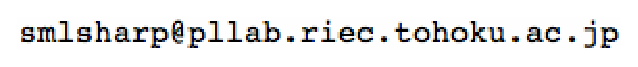
\epsfig{file=smlsharp-list.eps,width=0.4\textwidth}
共同研究の提案や各種問い合わせなどにご利用ください.
\end{itemize}
\else%%%%%%%%%%%%%%%%%%%%%%%%%%%%%%%%%%%%%%%%%%%%%%%%%%%%%%%%%%%%%%%%%%%%
	At present (April 2012), \smlsharp{} is developed by
\begin{itemize}
\item 
Atsushi Ohori(RIEC, Tohoku University)
\item 
Katsuhiro Ueno (RIEC, Tohoku University)
\end{itemize}
with help of graduate students.

	The past \smlsharp{} development team members include (with the
affiliation at the time of development):
\begin{itemize}
\item Atsushi Ohori (School of Information Science, JAIST; RIEC, Tohoku University)
\item Kiyoshi Yamatodani (Sanpukoubou Inc)
\item Nguyen Huu Duc (School of Information Science, JAIST; RIEC, Tohoku University)
\item Liu Bochao (School of Information Science, JAIST; RIEC, Tohoku University)
\item Satoshi Osaka (School of Information Science, JAIST)
\item Katsuhiro Ueno (School of Information Science, JAIST; RIEC, Tohoku University)
\end{itemize}

	Contact information regarding \smlsharp{}:
\begin{itemize}
\item \smlsharp{} home page:
\url{http://www.pllab.riec.tohoku.ac.jp/smlsharp/ja/}

\item \smlsharp{} mailing list:
{\tt smlsharp-list@pllab.riec.tohoku.ac.jp}

This list is for general discussion on \smlsharp{}.
We use Japanese and English in discussion.
To post a message, you need to subscribe to this list.
All the messages are made available on the Web.

How to subscribe:\url{http://www.pllab.riec.tohoku.ac.jp/mailman/listinfo.cgi/smlsharp-list?language=ja}\\
Mail archive:\url{http://www.pllab.riec.tohoku.ac.jp/pipermail/smlsharp-list/}

\item Email address of the \smlsharp{} development team :
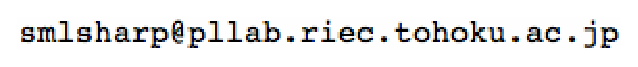
\epsfig{file=smlsharp-list.eps,width=0.4\textwidth}

Send your questions, requests and comments to us.
\end{itemize}
\fi%%%%<<<<<<<<<<<<<<<<<<<<<<<<<<<<<<<<<<<<<<<<<<<<<<<<<<<<<<<<<<<<<<<<<<

\section{\txt{謝辞}{Acknowledgments}}
\label{sec:acknowledgements}
	
\ifx\jp%>>>>>>>>>>>>>>>>>>>>>>>>>>>>>>>>>>>>>>>>>>>>>>>>>>>>>>>>>>>>>>>>>
	2003年にスタートしたSML#開発の過程では,以下を含む色々なご指導や
ご協力を頂きました.
	ここに謝意を表します.
\else%%%%%%%%%%%%%%%%%%%%%%%%%%%%%%%%%%%%%%%%%%%%%%%%%%%%%%%%%%%%%%%%%%%%
	From its start in 2003, we have benefited from many pepples.
	We acknowledge some of them below.
\fi%%%%<<<<<<<<<<<<<<<<<<<<<<<<<<<<<<<<<<<<<<<<<<<<<<<<<<<<<<<<<<<<<<<<<<
	
\subsection{\txt{プロジェクトファンディング}{Project Funding}}

\ifx\jp%>>>>>>>>>>>>>>>>>>>>>>>>>>>>>>>>>>>>>>>>>>>>>>>>>>>>>>>>>>>>>>>>>
	\smlsharp{}言語の研究開発は,2003年から5年間の文部科学省リーディ
ングプロジェクトe-Society基盤ソフトウェアの総合開発「高い生産性をもつ高
信頼ソフトウェア作成技術の開発」
(\url{http://www.tkl.iis.u-tokyo.ac.jp/e-society/index.html)}
の一つの課題
「プログラムの自動解析に基づく高信頼ソフトウェアシステム構築技術」(究代
表者:大堀 淳)としてスタートをきることができました.
	このプロジェクトの主要な目標が\smlsharp{}言語コンパイラの開発で
した.
	\smlsharp{}は開発ソースの総量が\smlsharpSize{}行を超える大規模シ
ステムです.
	このプロジェクトの支援がなければ,\smlsharp{}の開発は困難であっ
たと思われます.
	文部科学省,e-Societyの領域代表の片山卓也先生,および関係各位に
深謝いたします.
\else%%%%%%%%%%%%%%%%%%%%%%%%%%%%%%%%%%%%%%%%%%%%%%%%%%%%%%%%%%%%%%%%%%%%
	\smlsharp{} development was started as a part of the 5 year
project 
``e-Society leading project: highly productive reliable software
development technologies (Project Director: Professor Takuya Katayama)'' 
under the title
``
reliable software development technology based on automatic program analysis
(chief investigator: Atsushi Ohori)
''
(\url{http://www.tkl.iis.u-tokyo.ac.jp/e-society/index.html}).
\fi%%%%<<<<<<<<<<<<<<<<<<<<<<<<<<<<<<<<<<<<<<<<<<<<<<<<<<<<<<<<<<<<<<<<<<


\subsection{
\txt{\smlsharp{}が使用しているソフトウエア}
    {Third-party code used in \smlsharp{}}
}

\ifx\jp%>>>>>>>>>>>>>>>>>>>>>>>>>>>>>>>>>>>>>>>>>>>>>>>>>>>>>>>>>>>>>>>>>
	\smlsharp{}言語は,第\version{}版以降は,\smlsharp{}自身でコンパ
イルし開発を行なっていますが,それ以前は,Standard ML of New Jerseyおよ
びMLTonのStandard MLコンパイラを使って開発を行いました.

	\smlsharp{}は前節(\ref{sec:smlsharpTeam})の開発チー
ムによって開発されたソフトウェアです.
	ソースコードの殆どをスクラッチから開発しましたが,一部に以下のコー
ドを利用しています.

\begin{center}
\begin{tabular}{|c|c|c|}
\hline
内容 & \smlsharp{}ソース上の位置 & ソース
\\\hline
ML-Yacc & src/ml-yacc  & Standard ML of New Jersey (110.73)
\\\hline
ML-Lex & src/ml-lex  & Standard ML of New Jersey (110.73)
\\\hline
2分探索木関数 & src/smlnj-lib &  Standard ML of New Jersey (110.73)
\\\hline
TextIO,
BinIO,
OS,
Timer
の各structure
&
src/smlnj/Basis
&
Standard ML of New Jersey (110.73)
\\\hline
浮動小数点/
文字列変換関数
(dtoa.c)
&
src/runtime/netlib
&
the Netlib
\\\hline
SMLFormatの
SML文法定義
&
src/smlformat/generator/main/
&
Standard ML of New Jersey
\\\hline
\end{tabular}
\end{center}

	これらソースは,いずれも\smlsharp{}ライセンスと整合性あるライセ
ンスで配布されているオープンソースソフトウェアです.
	「\smlsharp{}ソース上の位置」にそれぞれのライセンスが添付されて
います.
\else%%%%%%%%%%%%%%%%%%%%%%%%%%%%%%%%%%%%%%%%%%%%%%%%%%%%%%%%%%%%%%%%%%%%
	After the \version{} version had completed, \smlsharp{} has been
developed by the \smlsharp{} compiler itself.
	Before the \version{} version, we have used Standard ML of New
Jersey and MLTon compilers.

	The \smlsharp{} compiler is a software developed by the
\smlsharp{} development team (\ref{sec:smlsharpTeam}).
	We have developed most of the code of \smlsharp{} compiler from
scratch, except for the following code:

\begin{center}
\begin{tabular}{|c|c|c|}
\hline
contents & location in \smlsharp{} distribution & source code
\\\hline
ML-Yacc & src/ml-yacc  & Standard ML of New Jersey (110.73)
\\\hline
ML-Lex & src/ml-lex  & Standard ML of New Jersey (110.73)
\\\hline
binary search tree & src/smlnj-lib &  Standard ML of New Jersey (110.73)
\\\hline
{\tt TextIO},
{\tt BinIO},
{\tt OS},
{\tt Timer}
structures
&
src/smlnj/Basis
&
Standard ML of New Jersey (110.73)
\\\hline
floating point-string conversion
(dtoa.c)
&
src/runtime/netlib
&
the Netlib
\\\hline
SML grammar definition used 
in SMLFormat tool
&
src/smlformat/generator/main/
&
Standard ML of New Jersey
\\\hline
\end{tabular}
\end{center}

	All of the above are open-source software that are compatible
with \smlsharp{} license.
	The \smlsharp{} source distribution includes the license of each
of them at the ``location in \smlsharp{} distribution'' show above.
\fi%%%%<<<<<<<<<<<<<<<<<<<<<<<<<<<<<<<<<<<<<<<<<<<<<<<<<<<<<<<<<<<<<<<<<<

\subsection{\txt{研究開発協力者}{Collaborators}}

\ifx\jp%>>>>>>>>>>>>>>>>>>>>>>>>>>>>>>>>>>>>>>>>>>>>>>>>>>>>>>>>>>>>>>>>>
	\smlsharp{}言語の開発にあたっては,多くの人々からの指導を受けま
した.
	過去現在の開発チーム(第(\ref{sec:smlsharpTeam})節)以外で特に
貢献のあった方々は以下の通りです.
\begin{itemize}
\item 篠埜功氏.
大堀と共に,関数フュージョン機能を持つ新たしいインラインの理論および
その実験的な実装を行いました.
	この機能は実験的な実装がありますが,まだ十分な完成度が得られてお
らず\smlsharp{}\version{}版に組み込まれていませんが,将来取り入れたいと
考えています.
\item 大友聡顕氏.
	大堀,上野と共に,オブジェクトを動かさないGCの研究開発に携わり,
初期の実験的な実装を行い,この方式が有望であることを確認しました.
	この成果は,現在のオブジェクトを動かさないGCの方式の開発と実装の
契機となったものです.
\end{itemize}
	これらの方々以外にも,\smlsharp{}は,大堀等との共同で行なった様々
な型理論やコンパイル方式の基礎研究を基に設計されています.
	現在の\smlsharp{}言語に直接生かされている出版された基礎研究成果
には以下のものが含まれます.
\begin{itemize}
\item レコード多相性の理論\cite{ohor92popl,ohor95toplas}.
\item データベースの型推論\cite{ohor88lfp}.
\item データベース言語(Machiavelli)\cite{ohor89sigmod,bune96tods}.
\item ランク1多相性の型理論\cite{ohor99icfp}.
\item MLのunboxed意味論\cite{ohor97unbox}.
\item MLにおける自然なデータ表現\cite{nguyen06ppdp}.
\item オブジェクトを動かさないGC\cite{ueno11icfp}.
\item 軽量の関数融合\cite{ohor07popl}.
\end{itemize}
	それ以外にも多くの共同研究者から色々な機会に示唆や助言を頂いてお
り,それらは1989年にまで遡りますが,それらの方々の列挙は割愛させてい
ただきます.
\else%%%%%%%%%%%%%%%%%%%%%%%%%%%%%%%%%%%%%%%%%%%%%%%%%%%%%%%%%%%%%%%%%%%%

	Many people have contributed to research and development of
\smlsharp{}.
	In addition to the development team (Section
\ref{sec:smlsharpTeam}),  the following people directly contributed to 
\smlsharp{} research.
\begin{itemize}
\item Isao Sasano.
With Atsushi Ohori, he investigated 
``Lightweight fusion by fixed point promotion'' and 
developed an experimental inlining module that performs lightweight
fusion.
	This feature is experimental and has not yet been integrated in
\smlsharp{} compiler, but we plan to adopt this method in a future
version.
\item Toshihiko Otomo.
	With Atsushi Ohori and Katsuhiro Ueno, he investigated the
possibility of non-moving collector and showed an initial experimental
result indicating that a non-moving GC is viable in functional
languages.
\end{itemize}
	Many other people helped us through collaborative research with
Atsushi Ohori and others to develop type-theory and compilation methods
that underlie \smlsharp{} compiler.
	\smlsharp{} compiler is directly based on the
following research results, some of them were collaboratively done.
\begin{itemize}
\item record polymorphism \cite{ohor92popl,ohor95toplas}.
\item database type inference \cite{ohor88lfp}.
\item database language (Machiavelli)\cite{ohor89sigmod,bune96tods}.
\item rank-1 polymorphism \cite{ohor99icfp}.
\item unboxed semantics of ML \cite{ohor97unbox}.
\item natural data representation for ML \cite{nguyen06ppdp}.
\item efficient non-moving GC\cite{ueno11icfp}.
\item lightweight fusion \cite{ohor07popl}.
\end{itemize}
	We have also benefited from many other researchers from 1989.
	We refrain from compiling a comprehensive list, which seems to
be impossible. 
\fi%%%%<<<<<<<<<<<<<<<<<<<<<<<<<<<<<<<<<<<<<<<<<<<<<<<<<<<<<<<<<<<<<<<<<<

\section{\txt{\smlsharp{}ライセンス}{\smlsharp{} License}}
\label{sec:smlsharpLicence}

Copyright (c) 2006 - 2012, Tohoku University.\\
All rights reserved.\\

Redistribution and use in source and binary forms, with or without
modification, are permitted provided that the following conditions are
met:

\begin{itemize}
\item 
  Redistributions of source code must retain the above copyright
  notice, this list of conditions and the following disclaimer. 
\item 
  Redistributions in binary form must reproduce the above
  copyright notice, this list of conditions and the following disclaimer
  in the documentation and/or other materials provided with the
  distribution. 
\item 
  Neither the name of Tohoku University nor the names of its
  contributors may be used to endorse or promote products derived from
  this software without specific prior written permission.  
\end{itemize}

THIS SOFTWARE IS PROVIDED BY TOHOKU UNIVERSITY AND CONTRIBUTORS "AS IS"
AND ANY EXPRESS OR IMPLIED WARRANTIES, INCLUDING, BUT NOT LIMITED TO,
THE IMPLIED WARRANTIES OF MERCHANTABILITY AND FITNESS FOR A PARTICULAR
PURPOSE ARE DISCLAIMED. IN NO EVENT SHALL TOHOKU UNIVERSITY OR
CONTRIBUTORS BE LIABLE FOR ANY DIRECT, INDIRECT, INCIDENTAL, SPECIAL,
EXEMPLARY, OR CONSEQUENTIAL DAMAGES (INCLUDING, BUT NOT LIMITED TO,
PROCUREMENT OF SUBSTITUTE GOODS OR SERVICES; LOSS OF USE, DATA, OR
PROFITS; OR BUSINESS INTERRUPTION) HOWEVER CAUSED AND ON ANY THEORY OF
LIABILITY, WHETHER IN CONTRACT, STRICT LIABILITY, OR TORT (INCLUDING
NEGLIGENCE OR OTHERWISE) ARISING IN ANY WAY OUT OF THE USE OF THIS
SOFTWARE, EVEN IF ADVISED OF THE POSSIBILITY OF SUCH DAMAGE.

\section{
\txt{\smlsharp{}第\version{}版の機能と制限}
{Limitations in \smlsharp{} version \version{}}
}


\ifx\jp%>>>>>>>>>>>>>>>>>>>>>>>>>>>>>>>>>>>>>>>>>>>>>>>>>>>>>>>>>>>>>>>>>
	我々開発チームは第\ref{sec:whatIsSmlsharp}節でのべた機能をすべて
開発し\smlsharp{}開発開始時に目標とした機能を実現しています.
	第\version{}版にその殆どが含まれていますが,以下の制約があります.
\begin{enumerate}
\item マルチコア上のネイティブスレッド.
	この機能は現時点では,十分にテストされていないため,デフォルトで
はオフになっています.
	システム構築時({\tt ./configure}時)に{\tt --enable-thread}
を指定すればオンになり,コンパイラはPOSIX thread対応のコードを生成します.
	POSIX thread APIを{\tt \_import}すれば,マルチコア上でネイ
ティブスレッドが動くはずです.

\item データベースサーバ.
	現在デフォルトでサポートされているデータベースサーバは
PostgreSQLのみです.
	MySQLも接続できることを確認しています.
	近い将来,複数のサーバへの接続機能および実行時の複数のサーバの同時
使用のサポートを行う予定です.

\item ターゲットアーキテクチャ.
	現在の\smlsharp{}コンパイラは,32ビットのインテルアーキテクチャ
(x86, IA-32)向けのコード生成器しかもっていません.
	将来,マルチターゲット化を行う予定です.
	特に,インテルの64ビット版への対応は,近い将来行う予定です.

\item Windows版の対話型ループの制約.
	\smlsharp{}\version{}版は,すべて一つのネイティブコードコンパイ
ラで動いています.
	対話型ループも,(1)ユーザ入力のコンパイル,
(2)現在のコンパイラにリンク,
(3)動的にロード,のサイクルによって実現されています.
	この中で(2)のリンクをWindowsシステム上で実現するためには,シ
ステムの制約上,これまでに作られたオブジェクトファイル毎にリンクのための
ファイルをコマンドラインで指定する必要があります.
	このファイル数が,対話型環境での入力に従って増えて行きます.
	そのため,Windows上の対話型環境の連続使用は,コマンドラインの最
大文字数によって制約されます.

\item 最適化.
	現在のバージョンには,インライニングや定数の伝播などの基本的な最
適化も十分に実装されていません.
	従って,コンパイル時間,コンパイルされたコードの実行時間もともに
十分とは言えません.
	現在,最適化の設計開発を開始しました.
	将来の版では,他の最適化コンパイラに比肩する速度が得られると期待
しています.
\end{enumerate}
\else%%%%%%%%%%%%%%%%%%%%%%%%%%%%%%%%%%%%%%%%%%%%%%%%%%%%%%%%%%%%%%%%%%%%
	We have successfully developed all the features listed in
Section~\ref{sec:whatIsSmlsharp}, which we had initially aimed at.
	The version \version{} contains most of them, with the following 
restrictions.
\begin{enumerate}
\item {\bf Optimization.}

	In this version, optimization is far from adequate; it does not
even implement standard ones such as inlining and constant propagation.
	So both the compilation time and the speed of generated code are
not very satisfactory.
	We have started design and development of optimizing \smlsharp{}
compiler, and hope that we will provide an optimized \smlsharp{}
compiler that is as fast as other mature compilers.

\item {\bf Interface language.}

	To support separate compilation, we have defined the interface
language for \smlsharp{} source code.
	This is our initial design and has a room of improvement.
	We hope to improve the interface language based on our experience
and other user's comments and requests.


\item {\bf Native thread support on malticore CPU.}

	This feature has not yet been well tested.
	So we set it off by default.
	To enable it, give {\tt --enable-thread} to {\tt ./configure}. 
	The compiler then generate thread-safe code.
	If you import OS thread-library through {\tt \_import}
declaration, your multithread code should run on multicore CPU.

	We have also completed development of a fully concurrent
non-moving GC.
	This has not been integrated in \version{} version.
	The GC in the \version{} version is a stop-the-world multithread
extension of the non-moving GC.
	We will replace this with a fully concurrent non-moving GC in
a future version.

\item {\bf SQL integration.}

	The current version only supports PostgreSQL.
	The available SQL constructs are also limited.
	In future version, we shall support fuller SQL syntax and
multiple servers including MySQL.

\item {\bf Target Architecture.}

	The current compiler only generates IA-32 code.
	We plan to replace our current backend with a multi-target one.

\item {\bf Interactive loop on Windows Systems.}

	\smlsharp{} realizes interactive loop by (1) compiling the input
to an object file, (2) linking with the currently running system to
generate a dynamically loadable file, and then (3) dynamically loading
the object code using {\tt dlopen}. 
	In Windows systems, performing the linking in step 2 requires
to specify a link information file for each of all the previous object
files.
	This implies that the command-line arguments to \smlsharp{}
compiler uses in step 2 keep increasing during the interactive session,
and will hit the limit of the command-line length. 
	At that point, the interactive session may stall.

\end{enumerate}
\fi%%%%<<<<<<<<<<<<<<<<<<<<<<<<<<<<<<<<<<<<<<<<<<<<<<<<<<<<<<<<<<<<<<<<<<

% \section{第1章の用語解説及ぶFAQ}
% \label{sec:glossary1}
% 
% \begin{description}
% \item[BSDスタイルライセンス] 
% 二次著作物に関する制限が少ないオープンソースソフトウェアライセンスの一つ.
% 
% BSDスタイルライセンスでは,ライセンス内容をドキュメント等に表示する限り,
% ソースおよびバイナリ形式をとわず,コードの使用,変更,再配布を認めている.
% これにより,二次著作物,つまりそのソフトを利用して作成される種々の製品を,
% 自由に作成し配布や販売することができる.
% 
% 正確にな内容は英文のBSDライセンス(BSD License,Berkeley Software
% Distribution License)を参照.
% 
% 
% \item[メタ] 
% 「後に」あるいは「越えて」といった位置を表すギリシャ語.
% この接頭語を含むギリシャ語metaphsicaがアリストテレスのよって書かれた名前
% の付けられなかった本の題名の代わに使われることによって,
% 「「自然学」の後に位置する本」という意味のmetaphsicaが,
% その本の内容である「哲学,形而上学(metaphisics)」
% を意味する用語として定着した.
% それに伴い,もともとの位置の概念であったmetaに,自然学を超越する
% という意味が与えられ,種々の分野で使用されようになった.
% たとえば言語学の分野では,metaは,通常の言語の使用を分析するために用いる
% 言語として使用される.
% \end{description}
% 
% FAQ:
% \begin{itemize}
% \item 
% {[Q]} \smlsharp{}の開発に参加したいのですが?\\
% {[A]} もちろん可能です.意欲のある方はご連絡ください.一緒にプログラミング
% 言語の色々な機能を実現していきましょう.今後,研究室以外の人々とのソース
% の共有や変更の管理等の体制を整えていく予定です.
% 
% \item  
% {[Q]} 東北大学電気通信研究所でプログラミングを学ぶことができますか?\\
% {[A]} 東北大学電気通信研究所の不タッフ(教授,准教授,助教)は,学部は工学
% 部,大学院は情報科学研究科または工学研究科大学院の教員を兼務し,工学部知
% 能情報システム総合学科の学部4年生,および教員の所属する情報科学研究科お
% よび工学研究科大学院の学生を受け入れています.大堀研究室は情報科学研究科
% の教員を兼務しています.
% 
% 学部の場合は,工学部知能情報システム総合学科に,大学院なら情報科学研究科
% に入学し大堀研究室を志望すれば,我々と一緒に\smlsharp{}やその他プログラ
% ミング言語及びデータベースの研究開発を思う存分行うことができます.
% 
% \end{itemize}

\part{\txt{チュートリアル}{Tutorials}}
\label{part:tutorial}

\chapter{\txt{\smlsharp{}プログラミング環境の準備}
{Setting up \smlsharp{} programming environment}
}
\label{chap:tutorialEnvironment}

\ifx\jp%>>>>>>>>>>>>>>>>>>>>>>>>>>>>>>>>>>>>>>>>>>>>>>>>>>>>>>>>>>>>>>>>>
	第2部では,\smlsharp{}でプログラミングをマスターするための
チュートリアルを提供します.
	まず\smlsharp{}プログラミング環境を整えましょう.
\else%%%%%%%%%%%%%%%%%%%%%%%%%%%%%%%%%%%%%%%%%%%%%%%%%%%%%%%%%%%%%%%%%%%%
	The part~\ref{part:tutorial} provides tutorials to get started
writing \smlsharp{} programs.

	Let us begin by setting up a programming environment.
\fi%%%%<<<<<<<<<<<<<<<<<<<<<<<<<<<<<<<<<<<<<<<<<<<<<<<<<<<<<<<<<<<<<<<<<<

\section{
\txt{Unix系OS,Emacsエディタ,その他ツールの整備}
    {Unix-family OS,Emacs,and other tools}}
\label{sec:tutorialEnvironmemt}
\ifx\jp%>>>>>>>>>>>>>>>>>>>>>>>>>>>>>>>>>>>>>>>>>>>>>>>>>>>>>>>>>>>>>>>>>
	プログラミングのためには,
\begin{itemize}
\item 使いやすい高機能エディタ
\item コンパイラとリンカー
\end{itemize}
を含むプログラミング環境が必要です.
	\smlsharp{}でのプログラミングに必要とされるプログラミング環境は,
\smlsharp{}コンパイラのインストールを除けば,C言語の場合と同様です.
	Javaなどの言語では,これらを統合した対象言語に特化したEclipseなど
の統合開発環境を使用する場合が多いですが,Cとの直接連携機能を用いたシス
テムプログラミングやSQLを使ったデータベース操作などの\smlsharp{}の先端機
能を駆使したプログラミングを十分に楽しむためには,以下のような標準的なプ
ログラミング環境を整えることを勧めます.

\begin{description}
\item[Unix系のOS] 
	高度なプログラム開発には,Linux,FreeBSD,Mac OS等のUnix
系OSが豊富なツールを含んでいて便利です.
	Windows系のOSがインストールされたPCの場合は,VMware,VirtualBoxなど
の仮想マシンを利用してLinuxなどの環境を容易に構築できます.
	Windows系OSでは,Cygwinでもほぼ同等の環境が得られます.
	Windows系OSで,Emacsが自由に使いこなせれば,MinGW(+MSYS)でも十
分にプログラミングを楽しむことができると思われます.

\item[Emacsエディタ]
	プログラミングにもっとも適したエディタの一つです.
	プログラミングは,テキスト形式の文を書き,コンパイルしテストをし,
修正する,という作業の繰り返しであり,その大部分の時間はテキストエディタ
との付き合いとなります.
	そこで,強力でカスタマイズ可能なテキストエディタの選択が重要です.
	Emacs系テキストエディタ(GNU Emacs,XEmacsなど)は,複数のバッファ
の操作,ディレクトリなどのファイルの管理,コンパイラなどのコマンド起動,
さらに,それらの柔軟なカスタマイズ機能を備えた強力なエディタであり,プロ
グラミングやLaTeX文書などの複雑で高度な文書の作成に最適なエディタです.
	使い始める時に少々練習が必用ですが,使いこなせば,プログラム開発
の強力な道具となります.
	Unix系OSでは通常デフォルトでインストール済みです.

\item[Cコンパイラ] 
	\smlsharp{}コンパイラは,x86アーキテクチャのネイティブコードにコ
ンパイルし,ソースコードをOS標準のオブジェクトファイルを作成し,さらに
それらをリンクし実行形式ファイルを作成します.
	この過程でGNU Cコンパイラ{\tt gcc}を通してリンカーを呼び出します.
	Unix系OSやCygwin,MinGWのインストール時にプログラム開発用に適し
たシステムを選択すれば標準でインストールされているはずです.

	\smlsharp{}プログラムのみをコンパイルしリンクする場合は,ユーザ
が直接{\tt gcc}コンパイラを呼び出す必要はありませんが,C言語との直接連携
機能を使いより高度なプログラミングを行うためにも,{\tt gcc}コンパイラに
慣れておくことをお勧めします.
\item[データベースシステム] 
	\smlsharp{}のデータベース機能を使用するにはデータベースシステムを
インストールする必要があります.
	第\version{}版では,PostgreSQLが実行時にバインドされます.
	データベースアクセス機能を使用するには,PostgreSQLをインストール
する必要があります.
	詳細はOSに依存しますが,いずれの場合も簡単にインストールできるは
ずです.
\end{description}

	第\ref{sec:tutorialInstall}節で説明する通り,Windowsのユーザ
に対しても,コンパイル済みのバイナリープログラムを用意しています.
	このバイナリを使用すれば,Windowsのコマンドプロンプトで
\smlsharp{}コマンドが使用可能になります.
	その場合でも,Windows上にEmacsをインストールすることをおすすめし
ます.
	Emacsが持つshell機能をを使えば,\smlsharp{}コンパイラだけでも,
十分にに本格的な\smlsharp{}言語のプログラムを楽しむことができるはずです.
\else%%%%%%%%%%%%%%%%%%%%%%%%%%%%%%%%%%%%%%%%%%%%%%%%%%%%%%%%%%%%%%%%%%%%
	To enjoy writing programs, you need to set up a programming
environment including 
\begin{itemize}
\item a good text editor, and
\item a compiler and a linker.
\end{itemize}
	The environment required for \smlsharp{} programming is
essentially the same as in any other programming, except of course for
the \smlsharp{} compiler.
	In Java and other languages, an integrated development
environment such as Eclipse is often used, but for \smlsharp{}
programming, we recommend the following standard system development
environments.

\begin{description}
\item[OS in the Unix family] 
	A Unix-family OS such as Linux, FreeBSD (including Mac OS)
provides a rich collection of programming tools.
	This would be your first choice.
	It is easy to set up Linux on Windows using a virtual machine
such as VMWare.
	Cygwin on Windows OS provides a similar environment.

	If you do not plan to develop a large system with various tools
such as {\tt make} and {\tt configure/autoconf} then
the combination of Emacs and MinGW (+ MSYS) on Windows would be a
reasonable alternative.
	
\item[Emacs editor]
	This is one of the best editor for programming, which is a
repeated process of editing an ASCII text file and and compiling it.
	In most of the time, you are interacting with your text editor.
	So choosing a highly custormisable high-performance editor is
important.
	Among various choices, we recommend one in the Emacs-family (GNU
Emacs, XEmacs).
	Emacs is a powerful custormisable text editor, but it can also 
perform command execution and file system management. 
	It requires some practice at the beginnings, but once you mastered
its basic functionality, it will become a powerful tool in programming.

\item[C compiler] 
	\smlsharp{} compiler generates x86 native code, create an
object file in a standard format (e.g. EFL), and then generate 
an executable code by lining object files with C libraries.
	In this process, it calls GNU C compiler {\tt gcc}.
	In Unix-family OS including Cygwin and MinGW set up for
system development, {\tt gcc} should be installed.

	If your purpose is to make a small program entirely within
\smlsharp{}, then you will not need to call {\tt gcc} directly.
	However, if you want to make a program of certain size and
complexity, you will need to call some library functions or to code up
in C for law-level manipulation of hardware.
	This is straightforward in \smlsharp{}.
	To exploit this feature, we recommend that you familiarize
yourself with C compiler.	
\item[database systems] 
	\smlsharp{} seamlessly integrates SQL.
	If you set up PostgreSQL, then you can use PostgreSQL databases
directly from your \smlsharp{} code.
\end{description}

	As we explain in Section~\ref{sec:tutorialInstall},
we prepared a binary package for Windows users.
	By installing this package, \smlsharp{} compiler can be used 
a Windows application.
	In this case, we recommend to install Emacs.
	With Emacs shell, you can enjoy \smlsharp{} programming more
comfortably.
\fi%%%%<<<<<<<<<<<<<<<<<<<<<<<<<<<<<<<<<<<<<<<<<<<<<<<<<<<<<<<<<<<<<<<<<<


\section{
\txt{\smlsharp{}コンパイラの構造とブートストラップ}
    {Bootstrapping the \smlsharp{} compiler }
}
\label{sec:tutorialBootstrap}

\ifx\jp%>>>>>>>>>>>>>>>>>>>>>>>>>>>>>>>>>>>>>>>>>>>>>>>>>>>>>>>>>>>>>>>>>
	この節は,\smlsharp{}コンパイラをインストールし使用する上で,理
解する必要はありませんが,やや時間がかかる\smlsharp{}コンパイラのインス
トール処理の理解や,さらにコンパイラの一般的な構造を理解する上で有用と思
います.

	\smlsharp{}\version{}版コンパイラは,\smlsharp{}言語で書かれた
ファイルを分割コンパイルし,インテルのIA-32ネイティブコードを生成します.
	対話型モードも,このコンパイラを使い,
(1)現在の環境下で分割コンパイル,
(2)システムとのリンク,
(3)オブジェクトファイルの動的ロード
を繰り返すことによって実現しています.
	\smlsharp{}コンパイラは\smlsharp{}言語とCで書かれており,
さらに自分自身のコンパイル時に以下のツールを使用しています.
\begin{itemize}
\item ml-lex,ml-yacc.字句解析および構文解析ツール.
\item SMLFormat.プリンタ自動生成ツール
\item 基本ライブラリ
\end{itemize}
	これらも\smlsharp{}言語で書かれています.

	\smlsharp{}コンパイラは,各\smlsharp{}ファイル(Standard MLファ
イルを含む)をシステム標準のオブジェクトファイルにコンパイルします.
	コンパイルしたファイルは,システム標準のリンカーやアセンブリプロ
グラムによって実行形式ファイルに変換できます.
	従って,\smlsharp{}コンパイラは,C言語のコンパイラと\smlsharp{}
コンパイラがあれば構築できます.
	しかし,もちろん,\smlsharp{}コンパイラを初めてインストールする
時には,\smlsharp{}コンパイラはまだ存在しません.
	このブートストラップの問題を解決し,\smlsharp{}を構築する標準の
手順は以下のとおりです.

\begin{enumerate}
\item \smlsharp{}コンパイラのソースコードをコンパイルするのに十分なコマ
ンド({\tt minismlsharp})を作るためのアセンブリファイルを用意.
\item インストールするシステムの下で,{\tt minismlsharp}のアセンブリファイルを
アセンブル・リンクし{\tt minismlsharp}コマンドを作成.
\item ML-lex,ML-yaccコマンドを生成.
\begin{enumerate}
\item {\tt minismlsharp}によってml-lex,ml-yaccが使用するライブラリソースをコンパイル
\item {\tt minismlsharp}によってml-lexとml-yaccのソースをコンパイル
\item システムリンカーによってml-lexとml-yaccのコマンドを生成.
\end{enumerate}
\item SMLFormatコマンドを生成
\begin{enumerate}
\item {\tt minismlsharp}によってSMLFormatが使用するライブラリソースをコンパイル
\item ml-yaccによってSMLFormatが使用するパーザーの\smlsharp{}ソースを生成
\item {\tt minismlsharp}によってSMLFormatのソースをコンパイル
\item システムリンカーによってSMLFormatを生成.
\end{enumerate}
\item \smlsharp{}コマンドの生成
\begin{enumerate}
\item {\tt minismlsharp}によって基本ライブラリ他すべてのライブラリソースをコンパイル
\item ml-yaccによって\smlsharp{}が使用するパーザーの\smlsharp{}ソースを生成
\item SMLFormatによって,\smlsharp{}が使用するプリンタの\smlsharp{}ソースを生成
\item {\tt minismlsharp}によって\smlsharp{}のソースをコンパイル
\item \smlsharp{}の実行時処理系が使用するCファイルをコンパイル
\item システムリンカーによってすべてのオブジェクトファイルをリンクし\smlsharp{}を生成.
\end{enumerate}
\item システムインストーラによって,以下のファイルをインストール
\begin{itemize}
\item ライブラリのオブジェクトファイル.分割コンパイルされたユーザプログ
ラムのインクに使用.
\item ライブラリのインターフェイスファイル.
ユーザプログラムのコンパイルに使用.
\item ライブラリのシグネチャファイル.ユーザプログラムのコンパイルに使用.
\item ml-lex,ml-yacc,SMLFormat,\smlsharp{}の各コマンド.
\end{itemize}
\end{enumerate}

	これらは以上のステップが示す様に,各ソースファイルやコマンド間に
は複雑な依存関係があります.
	さらに,いくつかのソースファイルの処理は,OSの環境に依存しています.
	これらは,大規模なシステムの典型です.
	これら依存関係を制御する一つの手法は,%システムで提供されている
GNU Autoconfによる{\tt configure}スクリプトと{\tt make}コマンドの使用です.
	\smlsharp{}コンパイラは,インターフェイスファイルに従って各ファイ
ルをコンパイルします.
	個別のファイルが必要とするファイルは,このインターフェイスファイル
に記述されています.
	\smlsharp{}コンパイラは,この依存関係を{\tt make}コマンドが読み
込めるフォーマットで出力する機能を持っています.
\begin{enumerate}
\item {\tt smlsharp -M $smlFile$}.
	ソースファイル$smlFile$を読み,このソースファイルをコンパイルする
ために必要なインターフェイスファイルのリストを{\tt Makefile}の形式で出力
します.
\item {\tt smlsharp -Ml $smiFile$}.
	インタフェイスファイル$smiFile$をトップレベルのファイルとみなし,
このトップレベルから生成されるべき実行形式コマンドのリンクに必要なオブジェ
クトファイルのリストを{\tt Makefile}の形式で出力します.
\end{enumerate}	

	\smlsharp{}システムは,この機能を利用して,上記の手順を実行する
{\tt Makefile}を生成しています.
	この{\tt Makefile}によって,通常の大規模システムの開発と同様,再
コンパイルが必要なファイルのみ{\tt make}コマンドによってコンパイル,リン
クが実行されます.

\else%%%%%%%%%%%%%%%%%%%%%%%%%%%%%%%%%%%%%%%%%%%%%%%%%%%%%%%%%%%%%%%%%%%%

	This section outlines the structure of \smlsharp{} compiler and
the method to building (bootstrap) it.
	You do not have to understand this section for installing
\smlsharp{} compiler, but you may find this section informative in
understanding various output during compilation of \smlsharp{} or 
compiler structure in general.

	\smlsharp{} system consists of a single compiler that performs
separate compilation. 
	Interactive mode is realized by the top-level-loop performing
the following:
\begin{enumerate}
\item compile the user input using the current static environment as its
interface,
\item link the object file with the external symbols in the current
system to generate a shared executable file,
\item dynamically load the shared executable in the current system.
\end{enumerate}

	\smlsharp{} is written in \smlsharp{} and C.
	In addition, it uses the following tools during compiling the
\smlsharp{} compiler.
\begin{itemize}
\item ml-lex,ml-yacc: a lexical analyzer generator and a parser generator.
\item SMLFormat: a printer generator.
\item The Standard ML Basis Library.
\end{itemize}
	All of them are written in Standard ML.

	\smlsharp{} compiler compiles each \smlsharp{} (which is a super
set of Standard ML) source file (source.sml) into a system standard
object file (sample.o file).
	The compiled files are then linked by the standard linker ({\tt
ld} in Unix-family OS) to generate an executable file.
	So, in order to build the \smlsharp{} compiler, it is sufficient
to have a C compiler and a \smlsharp{} compiler.
	But of course, at the time when the \smlsharp{} compiler is
first built, an \smlsharp{} compiler is not available.
	The standard step of solving this bootstrap problem is the
following.

\begin{enumerate}
\item {\bf Build {\tt minismlsharp} command.}
\begin{enumerate}
\item 
	Obtain a set of assembly source files of a minimal compiler
{\tt minismlsharp} that is sufficient for compiling all the source files
used in the \smlsharp{} compiler. 
	The assembly files are typically generated by a previous version
of \smlsharp{} compiler or some other Standard ML compiler. 
\item 
	In the system where the target \smlsharp{} compiler is
installed, assemble the {\tt minismlsharp} assembly files, link them
together and create the {\tt minismlsharp} command.
\end{enumerate}
\item {\bf Build ML-lex and ML-yacc commands.}
\begin{enumerate}
\item Compile the library files required by ml-lex and ml-yacc 
using {\tt minismlsharp}. 
\item Compile ml-lex and ml-yacc sources using {\tt minismlsharp}.
\item Create ml-lex and ml-yacc commands using the system linker.
\end{enumerate}
\item {\bf Build SMLFormat command.}
\begin{enumerate}
\item Compile the library files required for SMLFormat
using  {\tt minismlsharp}.
\item Generate the parser source file used in SMLFormat using ml-yacc
and ml-lex.
\item Compile SMLFormat source files using {\tt minismlsharp}.
\item Create SMLFormat command using the system linker.
\end{enumerate}
\item {\bf Build {\tt smlsharp} command.}
\begin{enumerate}
\item Compile all the library files using {\tt minismlsharp}.
\item Generate the parser source files of \smlsharp{} using ml-yacc and ml-lex.
\item Generate the printer source files of \smlsharp{} using SMLFormat.
\item Compile \smlsharp{} source files using {\tt minismlsharp}.
\item Compile C source files of \smlsharp{} runtime system.
\item Invoke the system linker to like all the object files.
	This yields \smlsharp{} command.
\end{enumerate}
\item {\bf Install the compiler.}
Use the system install command to install the following files.
\begin{itemize}
\item Library object files.
	They are linked with compiled user source files.
\item Library interface files.
	They are used when a user source file is compiled.
\item Library signature files.
\item ml-lex,ml-yacc,SMLFormat,\smlsharp{} commands.
\end{itemize}
\end{enumerate}

	As outlined above, there are complex dependencies among source
files and commands.
	Furthermore, processing some of these files depend on the
underlying OS.
	This is a typical situation in a large system development.
	One well established method to solve these dependency problems is
to use {\tt configure} script generated by GNU Autoconf and
{\tt make} command.

	\smlsharp{} compiler compiles each source file according to its
interface file, which describes the set of files require by the source
file.
	\smlsharp{} compiler can also generate a list of files on which
each source file is depend in the format processed by {\tt make}
command. 
	To let \smlsharp{} do this task, give it one of the following
switch.

\begin{enumerate}
\item {\tt smlsharp -M $smlFile$}.
	The compiler generates the dependency for the source file
$smlFile$ to be compiled in the {\tt Makefile} format.
します.
\item {\tt smlsharp -Ml $smiFile$}.
	The compiler assume that the interface $smlFile$ specifies the
top level system, and generate the list of necessary object files 
in the {\tt Makefile} format.
\end{enumerate}	

	The {\tt Makefile} that performs the above described complicated
sequence of compilation and linking steps to build the \smlsharp{}
compiler is generated by a script that uses the above functionality of
\smlsharp{}.
	Invoking {\tt make} command on {\tt Makefile} re-compiles only
the necessary files to build the \smlsharp{} compiler.
\fi%%%%<<<<<<<<<<<<<<<<<<<<<<<<<<<<<<<<<<<<<<<<<<<<<<<<<<<<<<<<<<<<<<<<<<

\section{
\txt{\smlsharp{}コンパイラのインストール}
    {Installing \smlsharp{} compiler}}
\label{sec:tutorialInstall}

\ifx\jp%>>>>>>>>>>>>>>>>>>>>>>>>>>>>>>>>>>>>>>>>>>>>>>>>>>>>>>>>>>>>>>>>>
	\smlsharp{}\version{}版は以下のプラットフォームで動作します.
\begin{itemize}
\item Linux(x86版.または32ビット開発環境のあるamd64版),
\item Mac OS X(Intel版),
\item WindowsのMinGW(32ビット版)
\end{itemize}

	また,\smlsharp{}のコンパイルと実行にはGMP(GNU Multiple Precision
Arithmetic Library)が必要です.
	GMPはLGPL(GNU Lesser General Public License)の下で配布されている
フリーソフトウェアです. 
	\smlsharp{}コンパイラおよび\smlsharp{}コンパイラが生成した実行形式
ファイルは,このライブラリを動的にリンクします.
	GMPは\smlsharp{}の配布パッケージには含まれていませんので,\smlsharp{}
コンパイラをインストールするユーザは,GMPを別途インストールする必要が
あります.
	多くの場合,OSのパッケージ管理システムなどで簡単に導入できるはずです.

	以上の環境があれば,\smlsharp{}は,簡単な手順でインストールでき
ます.
	以下に各OS毎のインストール処理の詳細は以下のとおりです.
\else%%%%%%%%%%%%%%%%%%%%%%%%%%%%%%%%%%%%%%%%%%%%%%%%%%%%%%%%%%%%%%%%%%%%
	The \smlsharp{} version \version{} works on one of the following
platform.
\begin{itemize}
\item Linux (x86, or amd64 with 32 bit development environment),
\item Mac OS X (Intel version),
\item MinGW (32 bit version) on Windows 
\end{itemize}


	The \smlsharp{} compiler uses GMP (GNU Multiple Precision
Arithmetic Library).
	GMP is an open-source software distributed under LGPL(GNU
Lesser General Public License).
	\smlsharp{} compiler and the executable programs compiled by the
\smlsharp{} dynamically link this library.
	GMP is not included in the \smlsharp{} distribution package.
	So you need to install it before installing \smlsharp.

	Below, we show the details of installation steps for each of the
supported operating systems.
\fi%%%%<<<<<<<<<<<<<<<<<<<<<<<<<<<<<<<<<<<<<<<<<<<<<<<<<<<<<<<<<<<<<<<<<<

\subsection{\txt{Mac OS X}{Mac OS X}}
\ifx\jp%>>>>>>>>>>>>>>>>>>>>>>>>>>>>>>>>>>>>>>>>>>>>>>>>>>>>>>>>>>>>>>>>>
	MacPortsのPortfileが用意されていますので,MacPortsを使って
インストールするのが最も簡単です.
	MacPortsをセットアップ後,\smlsharp{}のPortfileをダウンロードし,
ローカルなPortfileとして設定した上で,{\tt port install smlsharp} を実行すれば
インストールされます.
	詳細は,以下のとおりです.
\begin{enumerate}
\item 
\url{http://www.macports.org/}を参照し,
MacPorts をセットアップする.

\item 
	適当なディレクトリを作成し,ローカルなPortfileリポジトリとして設定する.
	例えば,ローカルなPortfileを {\tt /opt/var/macports/sources/local}
に置く場合は,そのディレクトリを作成した上で,
{\tt /opt/etc/macports/sources.conf}ファイルに
\begin{program}
file:///opt/var/macports/sources/local [nosync]
\end{program}
と記述する.
	詳しくは,
\url{http://guide.macports.org/#development.local-repositories}
を参照.

\item 
	下記URLより\smlsharp{}のPortfileのアーカイブをダウンロードする.
\url{http://www.pllab.riec.tohoku.ac.jp/smlsharp/download/smlsharp-macports.zip}

\item 
	ローカルPortfileリポジトリのディレクトリで上記アーカイブを展開する.
\begin{program}
\$ cd /opt/var/macports/sources/local\\
\$ unzip smlsharp-macports.zip
\end{program}
	この結果,{\tt lang/smlsharp/Portfile}が現れる.

\item
	 ローカルPortfileリポジトリのディレクトリに対して{\tt portindex}
コマンドを実行する.
\begin{program}
\$ portindex /opt/var/macports/sources/local
\end{program}

\item 
	以上で\smlsharp{}パッケージがMacPortsに設定されたので,{\tt
port}コマンドで\smlsharp{}コンパイラをインストールする.
\begin{program}
\$ port install smlsharp
\end{program}
\end{enumerate}

	\smlsharp{}は32ビットモード(x86アーキテクチャ)のみ対応しています.
	Mac OS X 10.6 以降で64ビット版のMacPortsを使う場合,
GMPライブラリなどの\smlsharp{}が必要とするソフトウェアも
32ビット版または32ビット版を含むユニバーサル
バイナリである必要があります.
	この依存関係は\smlsharp{}のインストールの際に{\tt port}コマンドに
よって自動的に解消されるはずです.
	この解消のために,{\tt port}コマンドはインストール済みの64ビット版
GMPライブラリなどをユニバーサルバイナリ化するために再ビルドする場合がある
ことに注意してください.

\else%%%%%%%%%%%%%%%%%%%%%%%%%%%%%%%%%%%%%%%%%%%%%%%%%%%%%%%%%%%%%%%%%%%%

	An \smlsharp{} Portfile is available.
	After setting up MacPorts,download the \smlsharp{} Portfile,
set it up as a local Portfile, and do {\tt port install smlsharp}.
	We show some more details below.

\begin{enumerate}
\item 
Consult \url{http://www.macports.org/} and set up MacPorts.

\item 
	Create a directory and set it as a local Portfile repository.
	For example, if you plan to put local Portfiles in
 {\tt /opt/var/macports/sources/local}, create the directory
and write
\begin{program}
file:///opt/var/macports/sources/local [nosync]
\end{program}
in the file {\tt /opt/etc/macports/sources.conf}.
	For more details, consult:
\url{http://guide.macports.org/#development.local-repositories}

\item 
	Download a Portfile archive from
\url{http://www.pllab.riec.tohoku.ac.jp/smlsharp/download/smlsharp-macports.zip}

\item 
	Extract the local Portfile repository in the repository
directory as:
\begin{program}
\$ cd /opt/var/macports/sources/local\\
\$ unzip smlsharp-macports.zip
\end{program}
	After this step, you will see {\tt lang/smlsharp/Portfile}.
\item
	 Execute {\tt portindex} command on the local Portfile
repository directory as:
\begin{program}
\$ portindex /opt/var/macports/sources/local
\end{program}

\item 
	The above steps should have set \smlsharp{} package to MacPorts.
	You can now install \smlsharp by {\tt port} command as:
\begin{program}
\$ port install smlsharp
\end{program}
\end{enumerate}

	\smlsharp{} version \version{} only support 32 bit mode on x86
architecture.
	So in Mac OS X 10.6 or later version with 64 bit MacPorts,
GMP library must be 32 bit version or a universal binary that include a
32 bit version.
	This dependency should be automatically resolved when you
install \smlsharp{} by {\tt port} command.
	To resolve this dependency, {\tt port} command may re-build 64-bit GMP
to make it as a universal binary.
\fi%%%%<<<<<<<<<<<<<<<<<<<<<<<<<<<<<<<<<<<<<<<<<<<<<<<<<<<<<<<<<<<<<<<<<<

\subsection{\txt{Windows上の{\tt MinGW}}{{\tt MinGW} on Windows}}

\ifx\jp%>>>>>>>>>>>>>>>>>>>>>>>>>>>>>>>>>>>>>>>>>>>>>>>>>>>>>>>>>>>>>>>>>
	32ビット版MinGW用のバイナリパッケージが,
\url{http://www.pllab.riec.tohoku.ac.jp/smlsharp/download/smlsharp-1.0.0-1-mingw32-bin.tar.lzma}
に用意されています.
	32ビット版MinGWのCコンパイラとGMPライブラリをセットアップした後,
このバイナリパッケージをMinGWのルートディレクトリで展開すれば,
\smlsharp{}コンパイラが使用可能になります.

	単に展開する代わりに以下の手順を実行すれば,\smlsharp{}コンパイ
ラがパッケージ管理下に入り,GMPなど必要なソフトウェアの自動インストールや,
将来のバージョンアップなどにも簡単に対応できるようになります.
\begin{enumerate}
\item MinGWのホームページを参考に,MinGWをセットアップする.
以下では,MinGWは
\begin{verbatim}
 C:\MinGW
\end{verbatim}
にインストールされたものと仮定する.
\item 
ファイル
\begin{verbatim}
 C:\MinGW\var\lib\mingw-get\data\profile.xml
\end{verbatim}
の{\tt <profile>}要素の中に以下の設定を書き加える.
\begin{verbatim}
 <repository uri="http://www.pllab.riec.tohoku.ac.jp/smlsharp/download/mingw32/%F.xml.lzma">
   <package-list catalogue="smlsharp-package-list" />
 </repository>
\end{verbatim}
\item 以下のコマンドを実行する.
\begin{program}
mingw-get update\\
mingw-get install smlsharp
\end{program}
\end{enumerate} 
\else%%%%%%%%%%%%%%%%%%%%%%%%%%%%%%%%%%%%%%%%%%%%%%%%%%%%%%%%%%%%%%%%%%%%
	A binary package for 32 bit MinGW is available from:
\url{http://www.pllab.riec.tohoku.ac.jp/smlsharp/download/smlsharp-1.0.0-1-mingw32-bin.tar.lzma}.
	After setting up a C compiler and GMP library for 32 bit MinGM,
simply extract the binary package in the MinGW root directory.

	Instead of simply extracting the binary package, you can make
the \smlsharp{} compiler managed by the package system.
% 
% 	単に展開する代わりに以下の手順を実行すれば,\smlsharp{}コンパイ
% ラがパッケージ管理下に入り,GMPなど必要なソフトウェアの自動インストールや,
% 将来のバージョンアップなどにも簡単に対応できるようになります.
\begin{enumerate}
\item Set up MinGW consulting MinGW home page.
	In this explanation, we assume that MinGW is installed at:
\begin{verbatim}
 C:\MinGW
\end{verbatim}

\item 
Add the description
\begin{verbatim}
 <repository uri="http://www.pllab.riec.tohoku.ac.jp/smlsharp/download/mingw32/%F.xml.lzma">
   <package-list catalogue="smlsharp-package-list" />
 </repository>
\end{verbatim}
to the {\tt <profile>} element in the file:
\begin{verbatim}
 C:\MinGW\var\lib\mingw-get\data\profile.xml
\end{verbatim}

\item Execute the following commands:
\begin{program}
mingw-get update\\
mingw-get install smlsharp
\end{program}
\end{enumerate} 
\fi%%%%<<<<<<<<<<<<<<<<<<<<<<<<<<<<<<<<<<<<<<<<<<<<<<<<<<<<<<<<<<<<<<<<<<

\subsection{\txt{ソースからビルドする場合}{Building from the source}}
\ifx\jp%>>>>>>>>>>>>>>>>>>>>>>>>>>>>>>>>>>>>>>>>>>>>>>>>>>>>>>>>>>>>>>>>>
	Linuxなどのその他システムではソースからビルドしてください.
	ソースからのビルドには,以下の開発ツールとライブラリが事前に
インストールされている必要があります.
\begin{enumerate}
\item プログラム開発用のツール群GNU binutils(GNU Binary Utilities).
\item gccのCコンパイラ.
\item make(GNU makeを推奨)
\item GMPのライブラリ本体とヘッダーファイル
\end{enumerate}
	64ビットOSを使う場合,これらのツールおよびライブラリの32ビット版が
必要です.

	32ビット版GMPライブラリがOSのパッケージシステムによって提供されて
いない場合,32ビット版GMPライブラリもソースからビルドする必要があります.
	GMPライブラリのWebページ \url{http://gmplib.org/} などからGMPの
ソースコードを入手,展開し,{\tt configure}に{\tt ABI=32}オプションを与える
ことで32ビット版GMPライブラリをビルドすることができます.
\begin{program}
\$ ./configure ABI=32
\$ make
\$ make install
\end{program}
	すでにインストールされているGMPライブラリとの衝突を防ぐためにも,
さらに{\tt --prefix}オプションなどを与えると良いでしょう.
	GMPのビルド方法についての詳細はGMPライブラリのドキュメントを参照
してください.


	以上の環境の下で,以下の手順で\smlsharp{}をソースからビルドします.
\begin{enumerate}
\item ソースパッケージ(
\url{http://www.pllab.riec.tohoku.ac.jp/smlsharp/download/smlsharp-\version{}.tar.gz}
)をダウンロード
\item 適当な\smlsharp{}ソースディレクトリを決め,そこに展開.
\item 適当な\smlsharp{}のインストールディレクトリを決める.そのディレクトリへのパスを$PATH$とする.
\item
	\smlsharp{}ソースディレクトリにて{\tt configure}スクリプトを実行する.
        このとき,64ビットOSでは,Cコンパイラおよびリンカが32ビット版となる
ように{\tt CC}および{\tt LD}を適切に設定する.

i386 Linux の場合:
\begin{program}
\$ ./configure --prefix=$PATH$
\end{program}
amd64 Linux の場合:
\begin{program}
\$ ./configure CC='gcc -m32' LD='ld -m elf\_i386' --prefix=$PATH$
\end{program}
\item

	マルチスレッドサポートを有効化したい場合は,{\tt ./configure}コマンド
に{\tt --enable-thread}スイッチを加える.
\item
	{\tt make}コマンドを実行しビルドとインストールを行う.
\begin{program}
\$ make\\
\$ make install
\end{program}
	システム管理の都合上,インストールされるファイルを
$PATH$とは異なるディレクトリ$PATH'$に出力させたい場合は,
{\tt make install}コマンドに{\tt DESTDIR=$PATH'$}オプションを指定する.
\end{enumerate}

	以上により,以下のファイルがインストールされます.
\begin{enumerate}
\item {\tt smlsharp}コマンド:{\tt $PATH$/bin/smlsharp}
\item {\tt smlformat}コマンド:{\tt $PATH$/bin/smlformat}
\item {\tt smllex}コマンド:{\tt $PATH$/bin/smllex}
\item {\tt smlyacc}コマンド:{\tt $PATH$/bin/smlyacc}
\item ライブラリファイル:{\tt $PATH$/lib/smlsharp/}ディレクトリ以下のファイル
\end{enumerate}
以下のコマンドで\smlsharp{}コンパイラが起動できるはずです.
\begin{program}
\$ $PATH$/bin/smlsharp
\end{program}

補足とヒント:
\begin{itemize}
\item 
	この手順は,時間がかかります.(例えば,ThinkPadのVMWare上の
Linux では,3時間以上かかるようです.)
	特に,yaccが生成した{\tt iml.grm.sml}と{\tt ml.grm.sml}の2つの
ファイルのコンパイルに時間がかかりますが,ループしているわけではありませ
ん.
	将来の最適化されたバージョンでは,(劇的に)改善されているとはず
です.
% \item 最後にリンクが成功すると,
% \begin{program}
% xxxx.o : In function `F45xxx':\\
% (xxxx) : warning: the use of `tmpnam' is dangerous, better use `mkstemp'
% \end{program}
% とのメッセージが出力されます.これで正常に終了しています.
\item マルチコアCPUをお使いの方は,GNU makeならば{\tt make}コマンドを実行
するとき{\tt -j\nonterm{n}}スイッチを指定すると,並列にコンパイルされ,
実行時間が短縮される場合があります.\nonterm{n}は並列度です.コアの数程度
に指定すると良い結果が得られると思います.
\end{itemize}

\else%%%%%%%%%%%%%%%%%%%%%%%%%%%%%%%%%%%%%%%%%%%%%%%%%%%%%%%%%%%%%%%%%%%%
	For Linux and other systems, you need to build from the source.
	To do this, the following tools and libraries are required:
\begin{enumerate}
\item GNU binutils(GNU Binary Utilities),
\item gcc C compiler,
\item make (GNU make is recommended), and
\item GMP library and its header file.
\end{enumerate}
	In a 64 bit OS, these tools and libraries must be of 32 bit version.

	If you 64 bit OS does not provide 32 bit GMP library package,
you need to build the 32 bit version from the source.
% 	32ビット版GMPライブラリがOSのパッケージシステムによって提供されて
% いない場合,32ビット版GMPライブラリもソースからビルドする必要があります.
	In that case, get the GML source from GML web page 
\url{http://gmplib.org/},
and {\tt configure} it with {\tt ABI=32} option as in the following:
\begin{program}
\$ ./configure ABI=32\\
\$ make\\
\$ make install
\end{program}
	If your system have a 64 bit version installed, then you may
want to specify the install location of the 32 bit version through
{\tt --prefix} option.
	See GMP document for more details.


	With these preparation, \smlsharp{} can be build by the
following steps.
\begin{enumerate}
\item Download the source distribution from:
\url{http://www.pllab.riec.tohoku.ac.jp/smlsharp/download/smlsharp-\version{}.tar.gz}
\item Select an \smlsharp source directory and extract the tar archive there.
\item Select an \smlsharp{} installation direction. Let $PATH$ be the path
to the directory.
\item
	In the \smlsharp{} source directory, execute {\tt configure} script.
	In a 64 bit OS,set {\tt CC} and {\tt LD} to 32 bit C compiler
and 32 bit linker, respectively.

In i386 Linux:
\begin{program}
\$ ./configure --prefix=$PATH$
\end{program}
In amd64 Linux:
\begin{program}
\$ ./configure CC='gcc -m32' LD='ld -m elf\_i386' --prefix=$PATH$
\end{program}
	To enable multithread support, given 
{\tt --enable-thread} switch to {\tt ./configure} script.

\item
	Do the following
\begin{program}
\$ make\\
\$ make install
\end{program}
\end{enumerate}

	The following files are installed.
\begin{enumerate}
\item {\tt smlsharp} command at {\tt $PATH$/bin/smlsharp}
\item {\tt smlformat} command at {\tt $PATH$/bin/smlformat}
\item {\tt smllex} command at {\tt $PATH$/bin/smllex}
\item {\tt smlyacc} command at {\tt $PATH$/bin/smlyacc}
\item library files in the {\tt $PATH$/lib/smlsharp/} directory.
\end{enumerate}
	If successful, you can invoke \smlsharp{} compiler by typing:
\begin{program}
\$ $PATH$/bin/smlsharp
\end{program}

Some hints:
\begin{itemize}
\item 
	This process compiles all the source files including those of
tools, and takes some time.
	If you have a CPU with $n$ cores and use GNU make, then try to
give {\tt -jm} ($m \le n$) switch to {\tt make} command for
parallel processing, where {\tt m} indicate the degree of parallelism. 
\end{itemize}
\fi%%%%<<<<<<<<<<<<<<<<<<<<<<<<<<<<<<<<<<<<<<<<<<<<<<<<<<<<<<<<<<<<<<<<<<

\section{
\txt{\smlsharp{}の対話型モードを使ってみよう}
    {Let's try \smlsharp{} interactive mode}}
\label{sec:tutorialInteractive}
\ifx\jp%>>>>>>>>>>>>>>>>>>>>>>>>>>>>>>>>>>>>>>>>>>>>>>>>>>>>>>>>>>>>>>>>>

	インストールが終了すると,\smlsharp{}コンパイラが{\tt smlsharp}
という名前のコマンドとして使用可能となります.
	このコマンドをコマンドシェルやEmacsのshellモードから起動すること
によって,\smlsharp{}プログラムをコンパイル,実行できます.
	もっとも簡単な使用法は,\smlsharp{}コンパイラを対話モードで実行
することです.
	{\tt smlsharp}を引数なしで起動すると,対話モードの起動要求とみな
し,起動メッセージを表示しユーザからの入力待ちの状態となります.
\begin{tt}
\begin{quote}
\$ smlsharp\\
SML\# version 1.0.0 (2012-04-06 JST) for x86-linux\\
\# 
\end{quote}
\end{tt}
	「{\tt \#\ }」は\smlsharp{}システムが印字するプロンプト文字です. 
	またこの文書では,シェル(コマンド)のプロンプトを「{\tt \$\ }」と仮定します

	この後,コンパイラは以下の処理を繰り返します.
\begin{enumerate}
\item 区切り文字{\tt ;}まで,端末からでプログラムを読み込む.
\item 読み込んだプログラムをコンパイルし,プログラムを呼び出し実行する.
\item プログラムが返す結果を表示する.
\end{enumerate}
	以下に簡単な実行例を示します.
\begin{tt}
\begin{quote}
\# "Hello";\\
val it = "Hello" : string
\end{quote}
\end{tt}
	最初の行がユーザの入力です.
	2行目が,ユーザの入力に対する\smlsharp{}システムの応答です.
	この例のように,コンパイラは,プログラムの実行結果に加えコンパイ
ラが推論した型を表示します.
	さらに,実行結果に名前をつけ,これに続くセッションで利用可能にし
ます.
	ユーザによる指定がなければ,{\tt it}という名前が付けられます.
\else%%%%%%%%%%%%%%%%%%%%%%%%%%%%%%%%%%%%%%%%%%%%%%%%%%%%%%%%%%%%%%%%%%%%

	Include the \smlsharp{} installation directory in your path, 
so that \smlsharp{} compiler is available by the name {\tt smlsharp}.
	If you invoke {\tt smlsharp} without any parameter, \smlsharp{}
compiler stars its interactive session by printing the following
message and wait for the user input.
\begin{program}
\$ smlsharp\\
SML\# version 1.0.0 (2012-04-06 JST) for x86-linux\\
\# 
\end{program}
	The ``{\tt \#\ }'' character is the prompt \smlsharp{} compiler
prints.
	In this document, we write ``{\tt \$\ }'' for the 
shell prompt.

	The compiler then repeat the following steps.
\begin{enumerate}
\item Read the user input up to ``{\tt ;}''.
\item Compile the input program, execute it.
\item Print the result.
\end{enumerate}
	The following is a simple example.
\begin{tt}
\begin{quote}
\# "Hello world";\\
val it = "Hello world" : string
\end{quote}
\end{tt}
	The first line the user input.
	The second line is the response of \smlsharp{} system.
	As seen in this example, the compiler print the result value with
its type, bind it to a name for subsequent use.
	If the user does not specify the name, the system uses  {\tt it}
as the default name.

\fi%%%%<<<<<<<<<<<<<<<<<<<<<<<<<<<<<<<<<<<<<<<<<<<<<<<<<<<<<<<<<<<<<<<<<<

\section{
\txt
{\smlsharp{}のコンパイルモードを試してみよう}
{Let's try \smlsharp{} compile mode}
}
\label{sec:tutorialCompile}
\ifx\jp%>>>>>>>>>>>>>>>>>>>>>>>>>>>>>>>>>>>>>>>>>>>>>>>>>>>>>>>>>>>>>>>>>
	\smlsharp{}コンパイラは,対話型以外に,Cコンパイラのようにファイ
ルをコンパイルすることができます.

	まず,簡単な例として,前節での入力{\tt \# "Hello world";\\}をファ
イル書いてコンパイルしてみましょう.
	そのために,{\tt hello1.sml}を以下のような内容で作成します.
\begin{program}
"Hello world";
\end{program}
	最後のセミコロンはあってもなくても同じです.
	この作成したファイルは,以下のようにしてコンパイルできます.
\begin{program}
\$ smlsharp hello1.sml\\
\$ file a.out\\
a.out: ELF 32-bit LSB executable, Intel 80386, version 1 (SYSV), dynamically linked (uses shared libs), for GNU/Linux 2.6.18, not stripped\\
\$
\end{program}
	\smlsharp{}は,引数としてファイル名のみが与えられると,Cコンパイ
ラ同様,そのファイルをコンパイル,リンクし実行形式ファイルを作成します.
	以上のようにシステム標準の実行形式ファイルが{\tt a.out}作成され
ていることが確認できます.
	作成されるファイル名は{tt -o}スイッチで指定できます.
\begin{program}
\$ smlsharp -o hello1 hello1.sml\\
\$ ls hello1*
hello1 hellp1.sml
\$ 
\end{program}
	作成したファイルは,通常のコマンドと同じように実行できます.
\begin{program}
\$ ./hello1\\
\$ 
\end{program}
	何も表示されませんが,これで正常です.
	ファイルのコンパイルでは,対話型モードと違い,結果の値と型を表示
するコードは付加されません.

	結果を表示したければ,結果を表示する関数を呼ぶ必要があります.
	そこで,{\tt hello2.sml}を以下のような内容で作成します.
\begin{program}
print "hello world!\verb|\|n"
\end{program}
	このファイルには,このファイルで定義していない{\tt print}関数が
使用されています.
	我々の意図は基本ライブラリで定義された{\tt print : string ->
unit}を使用することですが,{\tt print}は自由に再定義できますから,
\smlsharp{}コンパイラにとっては,名前{\tt print}が
基本ライブラリ関数の{\tt print}を指すとはかぎりません.
	そこでこのファイルをコンパイルするためには,{\tt print}が定義さ
れているファイルをコンパイラに通知する必要があります.

	このようにファイルに定義された名前以外の名前を使用するファイルを
コンパイルするためには,そのファイルで使用する名前が他のソースファイルで
定義されていることを,{\bf インターフェイスファイル}で宣言する必要があり
ます. 
	\smlsharp{}は,ソースファイル名に対応するインターフェイスファイル
{\tt "hello2.smi"}を探します.
	{\tt hello.sml}を実行するためには,以下の{\tt "hello2.smi"}ファ
イルを以下のように作成する必要があります.
\begin{program}
\verb|_|require "basis.smi"
\end{program}
	この宣言は,{\tt hello2.sml}がインターフェイスファイル{\tt
"basis.smi"}で宣言されている資源を必要としていることを表しています.
{\tt "basis.smi"}はStandard MLの基本ライブラリで定義されているすべての名
前が宣言されているインターフェイスファイルです.

	この用意の下で,以下のコマンドを実行すれば,実行形式プログラムが
作成されます.
\begin{program}
\$ smlsharp hello.sml -o hello\\
\$ ./hello\\
hello word!
\end{program}
\else%%%%%%%%%%%%%%%%%%%%%%%%%%%%%%%%%%%%%%%%%%%%%%%%%%%%%%%%%%%%%%%%%%%%
	In addition to interactive execution, \smlsharp{} compiler can
also compile a file and create an executable program, just like C
compiler.  

	As a simple example, let us write the previous user input
{\tt \# "Hello world";} into a file {\tt hello1.sml}:
\begin{program}
"Hello world";
\end{program}
	The trailing semicolon does not have any effect in a file.
	This file can be compiled as follows.
\begin{program}
\$ smlsharp hello1.sml\\
\$ file a.out\\
a.out: ELF 32-bit LSB executable, Intel 80386, version 1 (SYSV), dynamically linked (uses shared libs), for GNU/Linux 2.6.18, not stripped\\
\$
\end{program}
	When only a file name is given, \smlsharp{} compiles the file,
link it and creates an executable file, whose default name is {\tt
a.out}.
	The output file name can be specified by a {\tt -o} switch.
\begin{program}
\$ smlsharp -o hello1 hello1.sml\\
\$ ls hello1*\\
hello1 hellp1.sml\\
\$ 
\end{program}
	The generated executable file can then be executed.
\begin{program}
\$ ./hello1\\
\$ 
\end{program}
	Nothing is printed by this program.
	This is normal.
	When compiling a file, \smlsharp{} does not attach code to print
the result value and its type.
	If you want to see something printed, you need to write code
to print it explicitly.
	So let's create the file {\tt hello2.sml} containing:
\begin{program}
print "hello world!\verb|\|n"
\end{program}
	This file contains a function {\tt print} which is not defined
in this file.
	Our intention is that {\tt print} denotes the function
{\tt print : string -> unit} in Standard ML Basis Library.
	However, since name {\tt print} can be freely re-defined,
for \smlsharp{} compiler, it does not necessarily mean the  library
function.
	In order to compile {\tt hello2.sml}, you need to notify the
compiler where the name {\tt print} is defined.
	For this purpose, an {\bf interface file} must be created.

	When compiling {\tt hello2.sml}, \smlsharp{} searches for 
its interface file by its default name {\tt "hello2.smi"}.
	So to compile {\tt hello2.sml}, you need to create file {\tt
"hello2.smi"}.
	Its contents can be the following.
\begin{program}
\verb|_|require "basis.smi"
\end{program}
	This declares that {\tt hello2.sml} uses names that are defined
in the interface file {\tt "basis.smi"}, which is the system supplied
file containing the declarations of all the names defined in Standard ML
Basis Library.

	With this preparation, {\tt hello2.sml} is compiled as follows.
\begin{program}
\$ smlsharp hello.sml -o hello\\
\$ ./hello\\
hello word!\\
\end{program}
\fi%%%%<<<<<<<<<<<<<<<<<<<<<<<<<<<<<<<<<<<<<<<<<<<<<<<<<<<<<<<<<<<<<<<<<<

\section{
\txt{{\tt smlsharp}コマンドの起動モード}
{{\tt smlsharp} command modes}}
\label{sec:tutorialSmlsharpParameter}

\ifx\jp%>>>>>>>>>>>>>>>>>>>>>>>>>>>>>>>>>>>>>>>>>>>>>>>>>>>>>>>>>>>>>>>>>
	{\tt smlsharp}の主な実行モードは以下の4つです.
\begin{description}
\item[対話型モード]
{\tt smlsharp}をパラメタなしに起動すると,対話型セッションを実行します.
\item[コンパイル・リンクモード]
一つのソースファイルを指定して起動すると
そのファイルをコンパイルし,実行形式プログラムを作成します.
\item[コンパイルモード]
{\tt -c}スイッチを指定して起動すると,指定されたソースファイルをオブジェ
クトファイルにコンパイルします.
\item[リンクモード]
一つのインターフェイスファイル({\tt smi}ファイル)
を指定して起動すると,インターフェイスファイルに対応するソースファイルと
インターフェイスで参照されたすべてのソースファイルがコンパイル済みとみなし,
それらすべてのオブジェクトファイルをリンクし,実行形式プログラムを作成し
ます.
\end{description}
	これら実行を制御する起動スイッチとパラメタには以下のものが含まれ
ます.
\begin{description}
\item[--help] ヘルプメッセージをプリントし終了.
\item[-v] 種々のメッセージを表示.
\item[-o \nonterm{file}] 出力ファイル(オブジェクトファイル,実行形式ファイル)の名前を指定.
\item[-c]  コンパイルしオブジェクトファイルを生成.
\item[-S]  コンパイルしアセンブリファイルを作成.
\item[-M] コンパイルの依存関係を表示
\item[-MM] システムライブラリを除いたコンパイルの依存関係を表示
\item[-Ml] リンクの依存関係を表示
\item[-MMl] システムライブラリを除いたリンクの依存関係を表示
\item[-I \nonterm{dir}] ソースファイルのサーチパスの追加
\item[-L \nonterm{dir}] リンカーへのライブラリファイルのサーチパスの追加
\item[-l \nonterm{libname}]  リンク時にライブラリ<libname>をリンク
\item[-Wl,\nonterm{args}]  リンカーへ<args>をパラメタとして渡す
\end{description}
\else%%%%%%%%%%%%%%%%%%%%%%%%%%%%%%%%%%%%%%%%%%%%%%%%%%%%%%%%%%%%%%%%%%%%
	{\tt smlsharp} execution modes include the following.
\begin{description}
\item[interactive mode]
When {\tt smlsharp} is invoked without any parameter as:
\begin{program}
\$ smlsharp\\
SML\# version 1.0.0 (2012-04-06 JST) for x86-linux\\
\# 
\end{program}
it execute the interactive session.
\item[compile and link mode]
When {\tt smlsharp} is invoked with a single source file as:
\begin{program}
\$ smlsharp \nonterm{file}.sml\\
\$ 
\end{program}
it compiles the source file {\tt \nonterm{file}.sml}, link the resulting
object and creates an executable program (with the name {\tt a.out} by default).
\item[compile mode]
When {\tt smlsharp} is invoked with {\tt -c} switch as in:
\begin{program}
\$ smlsharp -c \nonterm{file1}.sml $\cdots$ \nonterm{fileN}.sml \\
\$ 
\end{program}
it compile the given files {\tt \nonterm{file1}.sml $\cdots$
\nonterm{fileN}.sml}
into object files {\tt \nonterm{file1}.o $\cdots$
\nonterm{fileN}.o}.
\item[link mode]
When {\tt smlsharp} is invoked with a single interface files:
\begin{program}
\$ smlsharp \nonterm{file}.smi \\
\$ 
\end{program}
it assumes that {\tt \nonterm{file}.smi} is a top-level interface file
and link all the object files corresponding to the interface files
referenced from {\tt \nonterm{file}.smi}, and generate an executable
file.
\end{description}
	\smlsharp{} also recognizes various command-line switches.
\begin{program}
\$ smlsharp --help
\end{program}
will print a help message describing available switches.
\fi%%%%<<<<<<<<<<<<<<<<<<<<<<<<<<<<<<<<<<<<<<<<<<<<<<<<<<<<<<<<<<<<<<<<<<

\chapter{\txt{MLプログラミング入門}{Introduction to ML programming}}
\label{chap:tutorialMlprogramming}

\ifx\jp%>>>>>>>>>>>>>>>>>>>>>>>>>>>>>>>>>>>>>>>>>>>>>>>>>>>>>>>>>>>>>>>>>
	\smlsharp{}言語は,Standard ML言語と後方互換性のあるプログラミン
グ言語です.
	\smlsharp{}の高度な機能を使いこなすために,本章でまず,Standard
MLプログラミングの基礎を学びましょう.

現在この章は未完です.
第\ref{sec:tutorialPolymorphicfunction}節に続き近い将来,以下の
節を追加する予定です.
\begin{quote}
パターンマッチングによる関数定義\\
リストプログラミング\\
高階のリスト処理関数\\
データ型の定義\\
パターンマッチングによるデータ型の利用\\
モジュールシステム\\
Structure\\
local宣言\\
signature制約\\
種々のデータ型ライブラリ\\
Functor
\end{quote}
\else%%%%%%%%%%%%%%%%%%%%%%%%%%%%%%%%%%%%%%%%%%%%%%%%%%%%%%%%%%%%%%%%%%%%
	\smlsharp{} is a super set of Standard ML.
	To write a program in \smlsharp{} exploiting its advanced
features, you must first learn Standard ML programming.
	This chapter provides ML programming tutorial for those who
first learn ML programming.

\begin{small}
This chapter is incomplete

Continuing Section \ref{sec:tutorialPolymorphicfunction}, the following 
sections will be added in near future.
\begin{quote}
list programming\\
higher-order functions for lists\\
data type definitions\\
pattern matching \\
overview of the module system\\
Structure\\
local declaration\\
signature constraint\\
various data types and libraries\\
functors
\end{quote}
\end{small}
\fi%%%%<<<<<<<<<<<<<<<<<<<<<<<<<<<<<<<<<<<<<<<<<<<<<<<<<<<<<<<<<<<<<<<<<<

\section{\txt{ML言語について}{The ML language family}}
\label{sec:mllanguage}

\ifx\jp%>>>>>>>>>>>>>>>>>>>>>>>>>>>>>>>>>>>>>>>>>>>>>>>>>>>>>>>>>>>>>>>>>
	\smlsharp{}はML系関数型プログラミング言語の一つです.
	本節では\smlsharp{}の理解のためにML言語の概要を説明します.

	ML言語はEdinburgh LCF\cite{gord79}のメタ言語({\bf M}eta {\bf
L}anguage)として開発されました.
	メタ言語とは,ある言語の分析や記述をするための言語のことです.
	プログラミング言語を変換したり処理するための言語もメタ言語とみな
すことができます.
	Edinburgh LCFは計算可能な関数(つまりプログラム)を対象とした一
種の定理証明システムであり,その対象となる関数はPPLAMBDAと呼ばれる型付ラ
ムダ計算で表現されました.
	LCF MLはPPLAMBDAのメタ言語,つまりPPLAMBDAで書かれたプログラムを操
作しするためのプログラミング言語でした.
	MLの名前はこの歴史的事実に由来しています.
	関数を表すラムダ式を柔軟に操作する目的のために,ML自身ラムダ計
算を基礎とする関数型言語として設計されました.
	さらにプログラムを操作するプログラムを柔軟にかつ信頼性を持って記
述するために,型の整合性を自動的に検査する型推論機構が初めて開発されまし
た.

	このLCF MLは,PPLAMBDAの操作言語にとどまらない汎用のプロ
グラミング言語として価値があることが認識され,CardelliによってLCFとは独
立したプログラミング言語としてのMLコンパイラが開始され,PDP11やVAX VMSな
どの上に実装され使用されました.
	その後,Milner,Harper,MacQueen等によってプログラミング言語とし
ての仕様策定の努力がなされ,さらにこの言語がEdinburgh大学によってCardelli
のML上に実装されました.
	これらの成果を踏まえ,Standard MLの仕様\cite{sml}が確定し,その
後改訂され現在のStandard ML言語仕様\cite{sml97}として完成しました.
\else%%%%%%%%%%%%%%%%%%%%%%%%%%%%%%%%%%%%%%%%%%%%%%%%%%%%%%%%%%%%%%%%%%%%
	\smlsharp{} is a programming language in the ML family.

	ML was first developed as a {\bf M}meta {\bf L}anguage of
Edinburgh LCF\cite{gord79} system. 
	The prefix {\em meta\/} in this particular usage probably traces
back to Greek phrase ``ta meta ta phusika'', which  simply denotes the
book placed after the phusika (Physics).
	The denoted book happens to be on philosophy (metaphysics), which
made this prefix receive a meaning of the (philosophical) attitude of
analyzing things beyond the ordinary way of thinking.
	In the context of languages, a meta language is a language used
to analyze the ordinary usage (writing/reading/speaking) of a language.
	Objects of LCF system are computable functions (programs)
represented by a language called PPLAMBDA.
	LCF ML was a meta language of PPLAMBDA, namely, a programming
language to manipulate PPLAMBDA expressions.

	ML's name as well as its features are originated from this
historical role of LCF ML. 
	For flexible manipulation of programs, ML itself was defined as
a functional language.
	In addition, a type inference system was first introduced in ML
for reliable manipulation of function terms.
	Since the success of LCF ML, ML has evolved as a general purpose
programming language, and several compilers have been developed.
	Based on these efforts, its specification is formally defined as
Standard ML \cite{sml,sml97}.
% 	このLCF MLは,PPLAMBDAの操作言語にとどまらない汎用のプロ
% グラミング言語として価値があることが認識され,CardelliによってLCFとは独
% 立したプログラミング言語としてのMLコンパイラが開始され,PDP11やVAX VMSな
% どの上に実装され使用されました.
% 	その後,Milner,Harper,MacQueen等によってプログラミング言語とし
% ての仕様策定の努力がなされ,さらにこの言語がEdinburg大学によってCardelli
% のML上に実装されました.
% 	これらの成果を踏まえ,Standard MLの仕様\cite{sml}が確定し,その
% 後改訂され現在のStandard ML言語仕様\cite{sml97}として完成しました.
\fi%%%%<<<<<<<<<<<<<<<<<<<<<<<<<<<<<<<<<<<<<<<<<<<<<<<<<<<<<<<<<<<<<<<<<<


\section{\txt{宣言的プログラミング}{Declarative programming}}
\label{sec:tutorialDeclarative}


\txt
{
	時折,関数型プログラミングは「宣言的」であると言われます.
	この言葉は厳密な技術的用語ではなく,プログラムが実現したいことそ
のものの記述するといった意味の曖昧性のある言葉です.
	しかし,これから書こうとするプログラムが表現すべきものがあらかじ
め理解されている場合,宣言的な記述は,より明確な意味を持ちます.
	
	書こうとするプログラムが入力を受け取り出力を返す関数と理解できる
場合,そのプログラムを,入力と出力の関係を表す関数として直接表現できれば,
より宣言的記述となり,したがってより分かりやすく簡潔なプログラムとなるは
ずです.
	MLは,この意味でより宣言的な記述を可能にするプログラミング言語と
いえます.
	MLプログラミングをマスターする鍵の一つは,この意味での宣言的プロ
グラミングの考え方を身につけることです.
}
{
	Functional programming is sometimes described as ``declarative
programming''.
	This is not a precise technical term.
	It generally implies that programs naturally and directly
express what they should realize.
% 	この言葉は厳密な技術的用語ではなく,プログラムが実現したいことそ
% のものの記述するといった意味の曖昧性のある言葉です.
	If the problem to be solved is procedural in nature then a
procedural description may well be declarative.
	However, when the thing to be represented by a program has a
well defined meaning, then declarative programming has more precise
meaning.
	
	When a program to be written is best understood as a function
that takes an input and returns a result, then functional programming
would be naturally declarative.
	In many cases, this way of modeling problems yields 
clean and readable programs.
	In this sense, ML is a language that promotes declarative
description.
	A key to master ML programming is to obtain a skill of writing
declarative code in this sense.
% 	MLプログラミングをマスターする鍵の一つは,この意味での宣言的プロ
% グラミングの考え方を身につけることです.
% 	簡単な例として,数学の教科書で学んだ階乗を計算するプログラムを考
% えてみましょう.
}

\txt
{
	簡単な例として,数学の教科書で学んだ階乗を計算するプログラムを考
えてみましょう.
	自然数$n$の階乗$n !$は,以下のように定義されます.
}
{
	As a simple example, consider the factorial function.
	The factorial of $n$,  $n !$, is defined by the following mathematical
equations.
}
\begin{eqnarray*}
0 ! &=& 1
\\
n ! &=& n \times (n - 1) !
\end{eqnarray*}
\txt
{
MLでは,このプログラムを以下のように記述できます.
}
{
In ML, it is coded below.
}
\begin{tt}
\begin{quote}
fun fact 0 = 1\\
\ \ \ \ \ | fact n = n * fact (n - 1)
\end{quote}
\end{tt}
\txt
{
	この宣言によって{\tt fact}と言う名前の関数が定義されます.
	この定義は``{\tt |}''によって区切られた2つの場合からなっています.
	上段は,引数が{\tt 0}の場合は{\tt 1}を返すことを表し,下段はそれ
以外の場合,引数{\tt n}と{\tt n - 1}の階乗とを掛けた結果を返すことを表し
ています.
	それぞれが,上記の階乗の定義とほぼ完全に一致していることがおわかりでしょう.
}
{
	This declaration defines a function named {\tt fact}.
	It consists of two cases separated by ``{\tt |}''.
	The first case says fact returns {\tt 1} if the parameter is
{\tt 0}, and the second case says it otherwise returns the multiple of
{\tt n} and the factorial of {\tt n - 1}.
	These two cases exactly corresponds to the mathematical
definition of this function.
}
	
\txt
{
	このような単純な関数に限らず,種々のプログラムを,その意図する意
味に従い宣言的な関数として表現できれば,複雑なプログラムをより簡潔かつ分
かりやすく書き下すことができるかもしれません.
	プログラミング言語MLは,この考え方に従い,大規模で複雑な計算をプ
ログラムする言語と言えます.
	以下に続く節で,その基本となる考え方を学んでいきましょう.
}
{
	Various programs other than such a very simple mathematical
function can be written in a concise and readable fashion if you
can represent it as a declarative function according to the intended
meaning.
	ML is a programming language that promotes this way of declarative
programming.
	In the subsequent sections, we learn the essence of ML
programming.
}
\section{
\txt{式の組み合わせによる計算の表現}
{Representing computation by composing expressions}
}
\label{sec:tutorialExpression}

\txt
{
	前節の階乗の計算では,引数が{\tt 0}の場合は{\tt 1}を返し,それ以
外の一般の{\tt n}の場合は,{\tt n * fact (n - 1)}を返すようにプログラム
されていました.
	このように,関数が返すべき値は,値を表す式で表現されます.
	最初の場合の{\tt 1}も,値そのものではなく,ゼロという値を表す式
とみなします.
	{\tt n * fact (n - 1)}は,変数{\tt n}と関数を含む式です.
	一般にML言語の大原則は,
\begin{quote}
MLのプログラミングは,必要な値をもつ式を定義することを通じて行う
\end{quote}
というものです.
}
{
	In the factorial example, the program returns {\tt 1} 
if the parameter is {\tt 0},and returns {\tt n * fact (n - 1)}
otherwise.
	In this way, the value returned by a function is represented by
an {\em expression}.
	{\tt 1} in the first case is also an expression representing
the natural number zero.
	{\tt n * fact (n - 1)} is an expression involving variable {\tt
n} and function application.
	The basic principle of ML programming is 
\begin{quote}
programming is done by defining an expression that represents the desired value
\end{quote}
}

\txt
{
	式は以下の要素を組み合わせて構成されます.
\begin{enumerate}
\item {\tt 0}などの定数式
\item 関数の引数やすでに定義されている値を表す変数
\item 関数呼び出し
\item 関数を含む種々のデータ構造の構成
\end{enumerate}
	1から3までの組み合わせは,高校などで慣れ親しんだ算術式と同じ構
造を持っています.
	以下にこれらを組み合わせた対話型プログラミングの例を示します.
}
{
	An expression consist of the following components:
\begin{enumerate}
\item constant such as {\tt 0}
\item variables representing function parameters and defined values
\item function applications (function calls)
\item functions and other data structure constructions
\end{enumerate}
	The items 1 through 3 are the same as in arithmetic expressions,
as seen in the following expressions.
}
\begin{tt}
\begin{quote}
\# val pi = 3.14;\\
val pi = 3.14 : real\\
\# val r = 1.5;\\
val r = 1.5 : real\\
\# 2.0 * pi * r;\\
val it = 9.41999999999 : real\\
\# pi * r * r;\\
val it = 7.06499999999 : real\\
\# r * (Math.sin (pi / 6.0));\\
val it = 0.749655153964 : real\\
\# Math.sqrt 2.0;\\
val it = 1.414213562373 : real\\
\# it  = Math.pow (2.0, 3.0);\\
val it = 8.0 : real\\
\# val negative = \verb|~|1.0;\\
val negative = \verb|~|1.0 : real
\end{quote}
\end{tt}
\ifx\jp%>>>>>>>>>>>>>>>>>>>>>>>>>>>>>>>>>>>>>>>>>>>>>>>>>>>>>>>>>>>>>>>>>
	{\tt Math.sqrt}および{\tt Math.pow}はそれぞれ
平方根とべき乗を計算する組込み関数です.
	最後の例のように,MLでは負の定数はチルダ記号{\tt ~}を先頭に付
けて表記します.
\else%%%%%%%%%%%%%%%%%%%%%%%%%%%%%%%%%%%%%%%%%%%%%%%%%%%%%%%%%%%%%%%%%%%%
	{\tt Math.sqrt $n$} and {\tt Math.pow($n$,$m$)} are primitive
functions to compute $\sqrt{n}$ and $n^m$ respectively.
	As in the last example, a negative constant is written by
prefixing with ``{\tt \verb|~|}''.
\fi%%%%<<<<<<<<<<<<<<<<<<<<<<<<<<<<<<<<<<<<<<<<<<<<<<<<<<<<<<<<<<<<<<<<<<

\ifx\jp%>>>>>>>>>>>>>>>>>>>>>>>>>>>>>>>>>>>>>>>>>>>>>>>>>>>>>>>>>>>>>>>>>
	もちろんこれら簡単な式以外にも,数学の式で書けるものであればMLで
プログラムできます.
	例えば中学校で学んだ通り,2次方程式$ax^2 + bx + c = 0$の一つの
解は(Firefoxなどで正常に表示できます),
\[
\frac{ -b + \sqrt{ b^{2} - 4 a c } }{2 a} 
\]
という式で表されますから,以下のようなプログラムとして書き下せます.
\begin{program}
(\verb|~| b + Math.sqrt(Math.pow(b,2.0) - 4.0 * a * c)) / 2.0 * a
\end{program}
	{\tt a},{\tt b},{\tt c}が定義されていれば,このプログラムは
以下のように$\frac{ -b + \sqrt{ b^{2} - 4 a c } }{2 a}$の値を計算します.
\else%%%%%%%%%%%%%%%%%%%%%%%%%%%%%%%%%%%%%%%%%%%%%%%%%%%%%%%%%%%%%%%%%%%%
	In addition to those simple expressions, any other mathematical
expressions can be coded in this fashion.
	For example, one of the quadratic formula of the equation
$ax^2 + bx + c = 0$ is (use Firefox to display this page)
\[
\frac{ -b + \sqrt{ b^{2} - 4 a c } }{2 a} 
\]
	This is directly written in ML as:
\begin{program}
(\verb|~| b + Math.sqrt(Math.pow(b,2.0) - 4.0 * a * c)) / 2.0 * a
\end{program}
	When {\tt a},{\tt b},{\tt c} are defined, this expression
computes $\frac{ -b + \sqrt{ b^{2} - 4 a c } }{2 a}$ as seen below.
\fi%%%%<<<<<<<<<<<<<<<<<<<<<<<<<<<<<<<<<<<<<<<<<<<<<<<<<<<<<<<<<<<<<<<<<<
\begin{program}
\# val a = 1.0;\\
val a = 1.0 : real\\
\# val b = \verb|~|1.0;\\
val b = \verb|~|1.0 : real\\
\# val c = \verb|~|6.0;\\
val c = \verb|~|6.0 : real\\
\# val x = (\verb|~| b + Math.sqrt(Math.pow(b,2.0) - 4.0 * a * c)) / 2.0 * a;\\
val x = 3.0 : real
\end{program}

\section{\txt{再帰的な関数}{Recursive functions}}
\label{sec:tutorialRecursion}
\txt
{
	前節のような定数,変数,組込み関数の組み合わせだけでは,もちろん,
複雑な問題を解くプログラムを記述することはできません.
	MLプログラミングの原則は式を書くことによってプログラムすることで
すが,その中で重要な役割を果たす式が関数を表す式です.
}
{
	As we learned, ML programming is done by writing expressions.
	Of course, it is not sufficient to program a solution to a
complex problem with constant, variables and primitive functions.
	The important expressions in ML programming are those that
represent functions.

}

\txt
{
	関数は,すでに第\ref{sec:tutorialDeclarative}節で学んだように,
\begin{program}
{\bf fun}\ {\it funName}\ {\it param} = {\it expr}
\end{program}
の構文で定義されます.
	この宣言以降,変数{\it funName}は,引数{\it param}を受け取り,式
{\it expr}の値を計算する関数として使用可能となります.
	例えば2次方程式の解の公式を表現する関数
\[
\mbox{$f(a,b,c)$} = \frac{ -b + \sqrt{ b^{2} - 4 a c } }{2 a} 
\]
は以下のように定義できます.
}
{
	As we learned in Section~\ref{sec:tutorialDeclarative}, a
function is defined by the following syntax:
\begin{program}
{\bf fun}\ {\it funName}\ {\it param} = {\it expr}
\end{program}
	After this declaration, the variable {\it funName} is bound to a
function that takes {\it param} as its argument and returns the result 
computed by {\it expr}.
	For example, a function that represent a quadratic formula
	例えば2次方程式の解の公式を表現する関数
\[
\mbox{$f(a,b,c)$} = \frac{ -b + \sqrt{ b^{2} - 4 a c } }{2 a} 
\]
can be written as follows.
}
\begin{program}
\# fun f(a,b,c) = (\verb|~|b + Math.sqrt(Math.pow(b,2.0) - 4.0 * a * c)) / 2.0 * a;\\
val root = fn : real * real * real -> real\\
\# f(1.0, ~8.0, 3.0);\\
val it = 7.605551275464 : real\\
\# f(1.0, 2.0, 3.0);\\
val it = nan : real
\end{program}
\txt
{
	最後の例{\tt nan}は,浮動小数点演算の結果正常な数が得られなかった時に返される
非数(not a number)です.
}
{
	{\tt nan} in the last line is a special floating point number
constant representing  ``not a number''.
}

\ifx\jp%>>>>>>>>>>>>>>>>>>>>>>>>>>>>>>>>>>>>>>>>>>>>>>>>>>>>>>>>>>>>>>>>>
	さらに,この{\tt fun}構文は再帰的な定義を許します.
	すなわち,この構文で定義される関数{\it funName}を,関数定義本体
{\it expr}の中で使用することができます.
	このような再帰的な関数定義は,以下のような手順で設計していけば,
通常の算術関数と同じように自然に定義できるようになります.
\begin{enumerate}
\item 関数{\it funName}の振る舞いをあらかじめ想定する.
\item 想定された振る舞いをする関数{\it funName}があると仮定し,
受け取った引数が{\it param}の場合に返すべきか値を表す式{\it expr}
を定義する.
\end{enumerate}
	例えば,第\ref{sec:tutorialDeclarative}節で紹介した階乗を計算す
る関数{\tt fact}は以下のように設計できます.
\begin{enumerate}
\item {\tt fact}を階乗を計算する関数と想定します.
\item 階乗を計算する関数{\tt fact}を使い,階乗の定義に従い,返すべき値を
以下のように定義する.
\begin{enumerate}
\item 引数が{\tt 0}の場合,0の階乗は1であるから,{\tt 1}を返す.
\item {\tt 0}以外の一般の引数{\tt n}の場合,階乗の定義から,
{\tt n * fact(n - 1)}を返す.
\end{enumerate}
\end{enumerate}
	この2つの場合を単に書き下せば,以下の定義が得られます.
\begin{tt}
\begin{quote}
\# fun fact 0 = 1\\
\verb|>| \ \ \ \ \ | fact n = n * fact (n - 1);\\
val fact = fn : int -> int
\end{quote}
\end{tt}
\else%%%%%%%%%%%%%%%%%%%%%%%%%%%%%%%%%%%%%%%%%%%%%%%%%%%%%%%%%%%%%%%%%%%%
	Moreover,this {\tt fun} syntax allows recursive function
definitions. 
	The function name {\it funName} being defined in this
declaration can be used in the defining body {\it expr} of this
declaration.

	A recursive function can naturally be designed in the following step.
% 	このような再帰的な関数定義は,以下のような手順で設計していけば,
% 通常の算術関数と同じように自然に定義できるようになります.
\begin{enumerate}
\item 
	Presume the expected behavior of the function 
{\it funName} for all the cases, and assume such function exists.
\item 
	For each case of the parameter {\tt param}, write the {\it expr}
using {\tt param} and {\tt funName}.
\end{enumerate}
	For example,function {\tt fact} defined in
Section~\ref{sec:tutorialDeclarative} is defined in the following
steps.
\begin{enumerate}
\item Assume that you have the function {\tt fact} that correctly
compute the factorial of any number.
\item Using {\tt fact}, write down the body of each case as follows.
\begin{enumerate}
\item if the parameter is {\tt 0}, then since $0!=1$, the {\tt expr} is {\tt 1}.
\item otherwise, from the definition of the factorial function, 
the {\tt expr} is {\tt n * fact(n - 1)}.
\end{enumerate}
\end{enumerate}
	This yields the following recursive function definition.
\begin{tt}
\begin{quote}
\# fun fact 0 = 1\\
\verb|>| \ \ \ \ \ | fact n = n * fact (n - 1);\\
val fact = fn : int -> int
\end{quote}
\end{tt}
\fi%%%%<<<<<<<<<<<<<<<<<<<<<<<<<<<<<<<<<<<<<<<<<<<<<<<<<<<<<<<<<<<<<<<<<<

\ifx\jp%>>>>>>>>>>>>>>>>>>>>>>>>>>>>>>>>>>>>>>>>>>>>>>>>>>>>>>>>>>>>>>>>>
	以上の考え方に従い種々の再起関数を簡単に定義できます.
	たとえば,すべての数の和を求める関数{\tt sum}や引数$n$に対して与
えられた定数$c$の$n$乗を計算する{\tt power}なども,これら関数がすでにあ
ると思うことによって,以下のように簡単に定義できます.
\begin{tt}
\begin{quote}
fun sum 0 = 0\\
\ \ \ \ \ | sum n = n + sum (n - 1)\\
fun power 0 = 1\\
\ \ \ \ \ | power n = c * power (n - 1)
\end{quote}
\end{tt}
	{\tt sum}や{\tt power}が想定した振る舞いをすると仮定すれば,
関数が返す値は正しいので,関数全体の定義も正しいことがわかります.
\else%%%%%%%%%%%%%%%%%%%%%%%%%%%%%%%%%%%%%%%%%%%%%%%%%%%%%%%%%%%%%%%%%%%%
	The summation function {\tt sum} and exponentiation  function {\tt
power}, for example, can be written by presuming that these functions
were already given.
\begin{tt}
\begin{quote}
fun sum 0 = 0\\
\ \ \ \ \ | sum n = n + sum (n - 1)\\
fun power 0 = 1\\
\ \ \ \ \ | power n = c * power (n - 1)
\end{quote}
\end{tt}
	Under the presumed behavior of {\tt sum} and {\tt power}, each
case correctly computes the expected value, the entire definitions
are correct.

	This is a recursive way of reasoning.
	Think in this recursive way, and you can naturally write various
recursive functions. 
\fi%%%%<<<<<<<<<<<<<<<<<<<<<<<<<<<<<<<<<<<<<<<<<<<<<<<<<<<<<<<<<<<<<<<<<<

\section{\txt{複数の引数を取る関数}{Functions with multiple arguments}}
\label{sec:tutorialMultiargfun}

\ifx\jp%>>>>>>>>>>>>>>>>>>>>>>>>>>>>>>>>>>>>>>>>>>>>>>>>>>>>>>>>>>>>>>>>>
	前節の{\tt power}関数はあらじめ定義された定数{\tt C}の指数乗を計算す
る関数でしたが,では,この指数の底{\tt C}も引数に加え,{\tt n}と{\tt C}
を受け取って{\tt C}の{\tt n}乗を計算する関数を定義するにはどうしたらよい
でしょうか.
	これには,2つの書き方があります.
	以下の対話型セッションでは,その型情報とともに示します.
\begin{tt}
\begin{quote}
\# fun powerUncurry (0,C) = 1\\
> \ \ \ \ \ | powerUncurry (n,C) = C * powerUncurry(n - 1,C)\\
val powerUncurry : int * int -> int\\
\# powerUncurry (2,3);\\
val it = 9 : int\\
\ \\
\# fun powerCurry 0 C= 1\\
> \ \ \ \ \ | powerCurry n C = C * (powerCurry (n - 1) C)\\
val powerCurry : int -> int -> int\\
\# powerCurry 2 3;\\
val it = 9 : int
\end{quote}
\end{tt}
	{\tt powerUncurry}の型情報{\tt int * int -> int}は,引数を組として
受け取り整数を返す関数であることを示しています.
	これに対して{\tt powerCurry}の型情報{\tt int -> int -> int}は,
引数を2つ順番に受け取り整数を返す関数であることを示しています.
	上の例から想像される通り,MLでは関数定義の引数は,その関数が使わ
れる形で書きます.
	例えば{\tt powerUncurry}は{\tt fun powerUncurry (C,n) = ...}と定
義されていますから,{\tt powerUncurry(2,3)}のように使います.
\else%%%%%%%%%%%%%%%%%%%%%%%%%%%%%%%%%%%%%%%%%%%%%%%%%%%%%%%%%%%%%%%%%%%%
	The function {\tt power} defined in the previous section
computers a power of $C$ for a given {\tt C}.
	There are two way of generalizing this function so that it takes 
both {\tt n} and {\tt C} and return $C^n$.
	They are shown in the following interactive session.
\begin{program}
\# fun powerUncurry (0,C) = 1\\
> \ \ \ \ \ | powerUncurry (n,C) = C * powerUncurry(n - 1,C)\\
val powerUncurry : int * int -> int\\
\# powerUncurry (2,3);\\
val it = 9 : int\\
\ \\
\# fun powerCurry 0 C= 1\\
> \ \ \ \ \ | powerCurry n C = C * (powerCurry (n - 1) C)\\
val powerCurry : int -> int -> int\\
\# powerCurry 2 3;\\
val it = 9 : int
\end{program}
	The type {\tt int * int -> int} of {\tt powerUncurry} indicates
that it is a function that takes a pair of integers and returns an
integer.
	In contrast, the type {\tt int -> int -> int} of {\tt
powerCurry} says that it is a function that takes an integer and return
a function of type {\tt int -> int}.
	As seen in these example, in ML, a function is defined in the
form where it will be used.
	For example, {\tt powerUncurry} is defined {\tt fun powerUncurry
(C,n) = ...} so it is used as {\tt powerUncurry(2,3)}.
\fi%%%%<<<<<<<<<<<<<<<<<<<<<<<<<<<<<<<<<<<<<<<<<<<<<<<<<<<<<<<<<<<<<<<<<<

\section{\txt{関数適用の文法}{Function application syntax}}
\label{sec:tutorialApplysyntax}

\ifx\jp%>>>>>>>>>>>>>>>>>>>>>>>>>>>>>>>>>>>>>>>>>>>>>>>>>>>>>>>>>>>>>>>>>
	{\tt powerUncurry}は,複数引数を取るC言語の関数と同様です.
	ML言語の強みは,これ以外に,{\tt powerCurry}にように
引数を順番に受け取る関数が書けることです.
	これを正確に理解するために,ここでMLの関数式の構文を復習しておき
ましょう.
	数学などの式では関数の利用(適用)は,関数の引数を括弧でかこみ
$f(x)$のように記述しますが,MLなどラムダ計算の考え方を基礎とした関数型言
語では,単に関数と引数を並べて{\tt f x}のように書きます.

	式の集合を$expr$で表すと,定数,変数,関数適用を含むMLの構文は一
部は,以下のような文法となります.
\begin{tt}
\begin{eqnarray*}
expr &\mbox{\ \ }::=& c                  \mbox{\myem\myem (定数)} \\
     &|& x                    \mbox{\myem\myem (変数)} \\
     &|& expr\mbox{\ } expr   \mbox{\ (関数適用)} \\
     &|& \cdots               \mbox{\myem\myem その他の構文}
\end{eqnarray*}
\end{tt}

	この構文規則のみでは関数適用式が続いた場合,その適用順番をきめる
ことができません.
	例えば,式に割り算の構文$expr / expr$と足し算
$expr + expr$
を導入した場合を考えてみましょう.
	この文法は,{\tt 60 / 6 / 2 + 1}のような式をゆるしますが,どの割り算
が先に行われるのかで2通りの解釈が可能です.
	この算術式では,通常左から括弧があるとみなし,{\tt ((60 / 10) /
2) + 1 }と解釈されます.
	このような解釈を,割り算の構文は「左結合」し,かつ足し算の構文より「結
合力が強い」,と言います.

	ラムダ計算を下敷きとした関数適用をもつ言語では,関数適用式に関し
て以下の重要な約束があります.
\begin{quote}
関数適用式は左結合し,その結合力は最も強い
\end{quote}
	関数式は左結合すると約束されているので,{\tt powerCurry 2 3}は
{\tt ((powerCurry 2) 3)}と解釈されます.
	一般に,{\tt e1\ e2\ e3\ $\cdots$\ en}と書いた式は
{\tt ($\cdots$ ((e1\ e2)\ e3)\ $\cdots$\ en)}とみなされます.
\else%%%%%%%%%%%%%%%%%%%%%%%%%%%%%%%%%%%%%%%%%%%%%%%%%%%%%%%%%%%%%%%%%%%%
	{\tt powerUncurry} is just like a C function taking a pair of
arguments.
	Unlike C and other procedural languages, ML also allows the
programmer to write a function that takes multiple arguments in a
sequence like {\tt powerCurry}.
	For proper understanding of this feature, let us review function
application syntax.
	In mathematics, function application is written as $f(x)$,
but in ML it is written as {\tt f x}, simply juxtaposing function and its
argument. 

	Let $expr$ be the expressions consisting of constants, variables
and function applications.
	Its syntax is given by the following grammar.
\begin{tt}
\begin{eqnarray*}
expr &\mbox{\ \ }::=& c                  \mbox{\myem\myem (constants)} \\
     &|& x                    \mbox{\myem\myem (variables)} \\
     &|& expr\mbox{\ } expr   \mbox{\ (function application)} \\
     &|& \cdots
\end{eqnarray*}
\end{tt}

	This grammar is ambiguous in the sequence of function
applications.
	To understand this problem, let us examine familiar arithmetic
expressions.
	Suppose we introduce 
$expr + expr$,
$expr - expr$, and
$expr * expr$
for integer addition, subtraction and multiplication.
	Then we can write {\tt 10 - 6 - 2} but this expression
itself does not determine the order of subtraction and addition, and as
two different results are possible: {\tt (10 - 6) - 2 = 2} 
or
{\tt 10 - (6 - 2) = 4} .
	As in elementary school arithmetic, ML interprets this 
as {\tt (10 - 6) - 2 = 2}.
	We say that the subtraction {\em associates to the left} or
{\em is left associative}.
	For anther example, ML interprets {\tt 10 + 6 * 2} as {\tt 10
+ (6 * 2)}.
	We say that the multiplication {\tt *} associates {\em stronger
than} addition {\tt +}.
	
	In ML and other lambda calculus based functional languages, 
there is the following important rule:
\begin{quote}
function application associates to the left and its associatibity is the strongest
\end{quote}
	{\tt e1\ e2\ e3\ $\cdots$\ en} is interpreted as {\tt ($\cdots$
((e1\ e2)\ e3)\ $\cdots$\ en)}.
	For example, {\tt powerCurry 2 3} is interpreted as {\tt
((powerCurry 2) 3)}.
\fi%%%%<<<<<<<<<<<<<<<<<<<<<<<<<<<<<<<<<<<<<<<<<<<<<<<<<<<<<<<<<<<<<<<<<<

\section{\txt{高階の関数}{Higher-order functions}}
\label{sec:tutorialHeigher-order-fun}

\ifx\jp%>>>>>>>>>>>>>>>>>>>>>>>>>>>>>>>>>>>>>>>>>>>>>>>>>>>>>>>>>>>>>>>>>
	{\tt powerCurry 2 3}は{\tt ((powerCurry 2) 3)}と解釈されるという
ことは,ML言語における以下の重要な性質を意味しています.
\begin{quote}
{\tt (powerCurry 2)}は関数である.
\end{quote}
	このようにMLでは,関数は{\tt powerUncurry}のように関数定義構文を通じて定義
された関数名だけではなくプログラムで作ることができます.
	このように返された値は,{\tt powerCurry}の例のように,使うことが
できます.
	さらに,名前を付けたら関数に渡したりすることができます.
	例えば,以下のようなコードを書くことができます.
\begin{quote}
\# val square = power 2;\\
val square = int -> int\\
\# squqre 3;\\
val it = 9 : int\\
\# fun apply f = f 3;\\
val apply : (int -> int) -> int\\
\# apply square;\\
val it = 9 : int
\end{quote}
	{\tt apply}に対して推論された型は,この関数が,関数を受け取って
整数を返す関数であることを示しています.

	以上の例から理解される通り,MLは以下の機能を持っています.
\begin{quote}
	関数は,整数型などのデータと同様,プ
ログラムが返すことができる値でああり,自由に受け渡し,使うことができる.
	特に関数は,別の関数を引数として受け取ることができる.
\end{quote}
	これが,「プログラムを式で定義していく」という大原則の下での,MLプ
ログラミングの最も重要な原則です.
	関数を返したり受け取ったりする関数を{\bf 高階の関数}と呼びます.
\else%%%%%%%%%%%%%%%%%%%%%%%%%%%%%%%%%%%%%%%%%%%%%%%%%%%%%%%%%%%%%%%%%%%%
	As we learned that {\tt powerCurry 2 3} is interpreted as {\tt
((powerCurry 2) 3)}. 
	This implies:
\begin{quote}
{\tt (powerCurry 2)} is a function.
\end{quote}
	In ML, functions can be generated by a program.
	{\tt powerCurry} is a program that takes an integer and return a
function.
	Generated functions can be named and passed to other functions.	
	For example, one can write the following code.
\begin{quote}
\# val square = power 2;\\
val square = int -> int\\
\# squqre 3;\\
val it = 9 : int\\
\# fun apply f = f 3;\\
val apply : (int -> int) -> int\\
\# apply square;\\
val it = 9 : int
\end{quote}
	The type of {\tt apply} means that this is a function that takes
a function on integers and return an integer.

	In summary, ML has the following power.
\begin{quote}
	Just like integers, functions are values that can be returned
from a function or passed to a function.
	In particular, a function can take a function as a parameter. 
% 	関数は,整数型などのデータと同様,プ
% ログラムが返すことができる値でああり,自由に受け渡し,使うことができる.
% 	特に関数は,別の関数を引数として受け取ることができる.
\end{quote}
	This is the important principle of ML under the fundamental
principle of ML programming saying that programs are expressions.
% 	これが,「プログラムを式で定義していく」という大原則の下での,MLプ
% ログラミングの最も重要な原則です.
	A function that takes a function as a parameter or return a
function is called a {\bf higher-order function}.
\fi%%%%<<<<<<<<<<<<<<<<<<<<<<<<<<<<<<<<<<<<<<<<<<<<<<<<<<<<<<<<<<<<<<<<<<


\section{\txt{高階の関数の利用}{Using higher-order functions}}
\label{sec:tutorialHeigher-order-use}


\ifx\jp%>>>>>>>>>>>>>>>>>>>>>>>>>>>>>>>>>>>>>>>>>>>>>>>>>>>>>>>>>>>>>>>>>
	MLでクールな,つまり読みやすくかつ簡潔なプログラミングを効率良く
書いていく鍵は,高階関数の機能を理解し,高階の関数を使い,式を組み合わせ
ていくことです.
	この技術の習得には,当然習熟が必要でこのチュートリアルで尽くせる
ものではありませんが,その基本となる考え方を理解することは重要と思います.
	そこで,以下,簡単な例を用いて,高階の関数の定義と利用に関する考
え方を学びましょう.

	数学で数列の和に関する$\Sigma$記法を勉強したと思います.
	この記法は以下のような等式に従います.
\begin{eqnarray*}
\sum_{k=1}^0 f(k) &=& 0\\
\sum_{k=1}^{n+1} f(k) &=& f(n) + \sum_{k=1}^{n} f(k)
\end{eqnarray*}
	高校の教科書などでこの記法を学ぶ理由は,もちろん,この$\Sigma$で
表現される働きに汎用性があり便利だからです.
	記法$\sum_{k=1}^n f(k)$の簡単な分析をしてみましょう.
\begin{itemize}
\item $\sum$記法には$k,n,f$の3つの変数が含まれる.
この中で$k$は,$1$から$n$まで変化することを表す仮の変数である.
\item 式$\sum_{k=1}^n f(k)$は,与えられた自然数$n$と関数$f$に
対して
$
f(1) + f(2) + \cdots + f(n)
$
の値を表す式である.
\end{itemize}
	従って,$\sum$は$n$と整数を引数とし整数を返す関数$f$を受け取る
関数,つまり高階の関数とみなすことができます.
	高階の関数をプログラミングの基本とするMLでは,この関数を以下のよ
うに直接定義可能です.
\begin{tt}
\begin{quote}
\# fun Sigma f 0 = 0\\
\ \ \ \ \ \ \ \ \  | Sigma f n = f n + Sigma f (n - 1)\\
val Sigma = fn : (int -> int) -> int -> int
\end{quote}
\end{tt}
この{\tt Sigma}を使えば,任意の自然数関数の和を求めることができます.
\begin{tt}
\begin{quote}
\# Sigma square 3:\\
val it = 14 : int\\
\# Sigma (power 3) 3:\\
val it = 36 : int
\end{quote}
\end{tt}
	高階の関数は,このようにひとまとまりの機能を表現する上で大きな力
をもちます.
	複雑なプログラムを簡潔で読みやすいMLのコードとして書き下していく
能力を身につける上で重要なステップは,ひとまとまりの仕事を高階の関数として
抜き出し,それらを組み合わせながら,式を作りあげていく技術をマスターする
ことです.
	後に第\ref{sec:tutorialPolymorphicfunction}節で説明するMLの多相
型システムは,このスタイルのプログラムをより容易にする機構といえます.
	この機構とともに,MLの高階関数を活用すれば,複雑なシステムを宣言
的に簡潔に書き下していくことができるようになるはずです.
\else%%%%%%%%%%%%%%%%%%%%%%%%%%%%%%%%%%%%%%%%%%%%%%%%%%%%%%%%%%%%%%%%%%%%
	The key to writing a cool, i.e.\ readable and concise program
efficiently is to understand the role of higher-order functions
and to compose expressions using higher-order functions.
% 	MLでクールな,つまり読みやすくかつ簡潔なプログラミングを効率良く
% 書いていく鍵は,高階関数の機能を理解し,高階の関数を使い,式を組み合わせ
% ていくことです.
	As in any programming skill, mastering higher-order functions
require certain amount of practice, and is beyond this tutorial.
	However, there are few basic concepts that are important in
writing expressions using higher-order functions.
	This tutorial attempt to exhibit them.
	In what follows, we learn these concepts through simple
examples.

	In high school mathematics, we have learned $\Sigma$ notation.
	This notation satisfies the following equations.
\begin{eqnarray*}
\sum_{k=1}^0 f(k) &=& 0\\
\sum_{k=1}^{n+1} f(k) &=& f(n) + \sum_{k=1}^{n} f(k)
\end{eqnarray*}
	The reason for learning this notation represent a useful
abstraction, i.e.\ summing up a sequence of expressions with integer
indexes.
% 	高校の教科書などでこの記法を学ぶ理由は,もちろん,この$\Sigma$で
% 表現される働きに汎用性があり便利だからです.
	A brief analysis of the notation $\sum_{k=1}^n f(k)$ reveals the
following.
\begin{itemize}
\item The notation contains 3 variables $k,n,f$.
	Among them, $k$ is a variable only to indicate that
expressions are index by $k=1,\ldots,n$, and is not a free variable. 
	This is an expression containing two variables $n,f$.
\item Expression $\sum_{k=1}^n f(k)$ denotes the value
$
f(1) + f(2) + \cdots + f(n)
$
for any given integer $n$ and a function $f$.
\end{itemize}
	$\sum$ is a function that takes an integer $n$ and a function
$f$ that takes an integer and returns an integer, i.e.\ it is a
higher-order function.
% 	高階の関数をプログラミングの基本とするMLでは,この関数を以下のよ
% うに直接定義可能です.
	In ML, this higher-order function is directly code as follows.
\begin{program}
\# fun Sigma f 0 = 0\\
\ \ \ \ \ \ \ \ \  | Sigma f n = f n + Sigma f (n - 1)\\
val Sigma = fn : (int -> int) -> int -> int
\end{program}
	This {\tt Sigma} can compute the summation of any inter function.
\begin{program}
\# Sigma square 3:\\
val it = 14 : int\\
\# Sigma (power 3) 3:\\
val it = 36 : int
\end{program}

	As demonstrated by this example, higher-order functions has the
power of representing a useful computation pattern by abstracting its
components as argument functions.
	The key to writing a cool ML code is to master the skill of
abstracting useful computation patterns as higher-order functions.
	Polymorphic typing we shall learn in Section
\ref{sec:tutorialPolymorphicfunction} can be regarded as a mechanism to
support this style of programming. 
	Higher-functions with their polymorphic typing enable the ML
programmer to code a complicated system in a concise and declarative
way.
% 	この機構とともに,MLの高階関数を活用すれば,複雑なシステムを宣言
% 的に簡潔に書き下していくことができるようになるはずです.

% 	高階の関数は,このようにひとまとまりの機能を表現する上で大きな力
% をもちます.
% 	複雑なプログラムを簡潔で読みやすいMLのコードとして書き下していく
% 能力を身につける上で重要なステップは,ひとまとまりの仕事を高階の関数として
% 抜き出し,それらを組み合わせながら,式を作りあげていく技術をマスターする
% ことです.
% 	後に第\ref{sec:tutorialPolymorphicfunction}節で説明するMLの多相
% 型システムは,このスタイルのプログラムをより容易にする機構といえます.
% 	この機構とともに,MLの高階関数を活用すれば,複雑なシステムを宣言
% 的に簡潔に書き下していくことができるようになるはずです.
\fi%%%%<<<<<<<<<<<<<<<<<<<<<<<<<<<<<<<<<<<<<<<<<<<<<<<<<<<<<<<<<<<<<<<<<<

\section{\txt{MLにおける手続き的機能}{Imperative features of ML}}
\label{sec:tutorialImperative}

\ifx\jp%>>>>>>>>>>>>>>>>>>>>>>>>>>>>>>>>>>>>>>>>>>>>>>>>>>>>>>>>>>>>>>>>>
	これまで学んできた通り,式の組み合わせでプログラムを構築していく
ML言語はプログラムを宣言的に書く上で最も適した言語の一つです.
	これまでに,$\sum$関数などの算術演算を行う関数を例に説明しました
が,第\ref{sec:tutorialDeclarative}節で説明した通り,宣言的とは,意図す
る意味をできるだけそのまま表明するということであり,決して数学的な関数と
してプログラムを書いていくことが望ましい,との表明ではありません.

	もし,実現しようとしている機能が,手続き的な操作によって最も簡潔
に表現し理解できるなら,その手続きをそのまま表現するのが望ましいはずです.
	例えば,みなさんが今ご覧のディスプレイに文字を表示する操作は,こ
れまでに書かれている内容を別な情報で上書きする操作であり,具体的には,
ディスプレイのバッファを書き換える手続き的な操作です.
	ディスプレイに限らず,外部との入出力処理は,外部の状態に依存する
本質的に手続き的な操作です.
	そのほか,例えば新しい名前や識別子の生成などの処理,さらに,
サイクルのあるグラフの変換なども,手続き的なモデルで理解しプログラムした
ほが,より宣言的な記述になる場合が多いと言えます.

	このような操作をプログラムで簡潔で分かりやすく表現するには,
手続き的な処理が記述できたほうが便利です.
	式の組み合わせでコードを書いていくことが基本である関数型言語にこ
のような手続き的な処理を導入するために必要なことは,以下の2つです.
\begin{enumerate}
\item 状態を変更する機能の導入.
	例にあげたディスプレイの表示内容は,抽象的にはディスプレイの状態
と捉えることができます.
	手続き的なプログラムの基本は,この状態を変更することをくり返し目
的とする状態を作りだすことです.
	そのためには,変更可能なデータが必要となります.
\item 評価順序の確定.
	ディスプレイの表示内容の変更操作が複数あった場合,それらの適用順
序によって,どのような像が見えるかが決まります.
	従って,手続き的なプログラムを書くためには,変更操作がどの順に行
われるかに関する知識と制御が必要となります.
\end{enumerate}
	MLには,これら2つが関数型言語の枠組みの中に導入されています.
\else%%%%%%%%%%%%%%%%%%%%%%%%%%%%%%%%%%%%%%%%%%%%%%%%%%%%%%%%%%%%%%%%%%%%
	ML is a language where programs are defined by composing
expressions, and is suitable for declarative programming.
	So far we have used numerical functions such as $\sum$, but as
pointed out in Section \ref{sec:tutorialDeclarative},the intention of
declarative programming is to write what the program should express
directly as a code, and not intend to define a program as a mathematical
function.

	If the actual problem is best expressed as a sequence of
procedure, then directly writing done that sequence would be most
declarative.
	For example, displaying a sentence on the video display you are
looking at is the process to override the previous sentence with the new
sequence of characters.
	In an actual implementation, this is done by modifying the frame
buffer of the video screen hardware.
	This process is inherently procedural, and therefore best
described as a process to update the buffer.
	Input from and output to external world inevitably have this
property.
	For those problems, procedural representation would be most
direct and therefore concise and readable, thus declarative.
	
	Integrating imperative features in a functional language
requires the following.
\begin{enumerate}
\item Introduction of updating a mutable state.
	In the previous display example, display contents can be
understood as the state of the display.
	The basis of imperative programming is to update states to
obtain the desired state.
	For this, the introduction of mutable data structures is
required.
\item A predictable evaluation order.
	In the display example, the order of updates determine the image
and its motion in the display.
	To write a procedural program, it is necessary to control the
order of update operations.
% 	ディスプレイの表示内容の変更操作が複数あった場合,それらの適用順
% 序によって,どのような像が見えるかが決まります.
% 	従って,手続き的なプログラムを書くためには,変更操作がどの順に行
% われるかに関する知識と制御が必要となります.
% 	ディスプレイの表示内容の変更操作が複数あった場合,それらの適用順
% 序によって,どのような像が見えるかが決まります.
% 	従って,手続き的なプログラムを書くためには,変更操作がどの順に行
% われるかに関する知識と制御が必要となります.
\end{enumerate}
	ML introduces these two in a framework of functional programming.
\fi%%%%<<<<<<<<<<<<<<<<<<<<<<<<<<<<<<<<<<<<<<<<<<<<<<<<<<<<<<<<<<<<<<<<<<

\section{
\txt{変更可能なメモリーセルを表す参照型}
    {Mutable memory reference types}}
\label{sec:tutorialRef}

\ifx\jp%>>>>>>>>>>>>>>>>>>>>>>>>>>>>>>>>>>>>>>>>>>>>>>>>>>>>>>>>>>>>>>>>>
	MLには,以下の型と関数が組み込まれています.
\begin{tt}
\begin{quote}
type 'a ref\\
val ref : 'a -> 'a ref\\
val ! : 'a ref -> 'a\\
val := : 'a ref * 'a -> unit
\end{quote}
\end{tt}
	型{\tt 'a ref}は「'aの値への参照」を表す型です.
	参照とはポインタのことです.
	関数{\tt ref}は,任意の型{\tt 'a}の値を受け取り,その値への参照
を作成し返す関数です.
	関数{\tt !}は,参照を受け取りそれが指す値を返す関数です.
	関数{\tt :=}は代入を行う関数,すなわち,参照と値を受け取り,参照
が指す値を受け取った値に変更する関数です.
	以下は,参照型を使用した対話型セッションの例です.
\begin{tt}
\begin{quote}
\#val x = ref 1;\\
val x = \_ : int ref\\
\# !x;\\
val it = 1 : int\\
\# x := 2;\\
val it = () : unit\\
\# !x;\\
val it = 2 : int
\end{quote}
\end{tt}
	この参照型を,状態を参照として保持することにより状態に依存する処
理などの本質的に手続き的な処理を,通常の関数として書くことができます.
\else%%%%%%%%%%%%%%%%%%%%%%%%%%%%%%%%%%%%%%%%%%%%%%%%%%%%%%%%%%%%%%%%%%%%
	ML has the following type constructor and primitives.
\begin{tt}
\begin{quote}
type 'a ref\\
val ref : 'a -> 'a ref\\
val ! : 'a ref -> 'a\\
val := : 'a ref * 'a -> unit
\end{quote}
\end{tt}
	{\tt 'a ref} is a type of references (pointers) of type {\tt 'a}.
	Function {\tt ref} takes a value of type {\tt 'a} and returns a
reference to it.
	Function {\tt !} takes a reference and returns the value of that
reference.
	Function {\tt :=} assigns a given value to a given reference.
	This destructively update the reference cell.
	The following shows an interactive session manipulating a reference.
\begin{tt}
\begin{quote}
\#val x = ref 1;\\
val x = \_ : int ref\\
\# !x;\\
val it = 1 : int\\
\# x := 2;\\
val it = () : unit\\
\# !x;\\
val it = 2 : int
\end{quote}
\end{tt}
	A function performing imperative operation can be written by
maintaining a state using a reference.
% 	この参照型を,状態を参照として保持することにより状態に依存する処
% 理などの本質的に手続き的な処理を,通常の関数として書くことができます.
\fi%%%%<<<<<<<<<<<<<<<<<<<<<<<<<<<<<<<<<<<<<<<<<<<<<<<<<<<<<<<<<<<<<<<<<<

\section{
\txt{作用順,左から右への評価戦略}
    {Left-to-right applicative order evaluation}
}
\label{sec:tutorialSideeffect}

\ifx\jp%>>>>>>>>>>>>>>>>>>>>>>>>>>>>>>>>>>>>>>>>>>>>>>>>>>>>>>>>>>>>>>>>>
	手続き的処理を書くためにはプログラムの各部分の実行順序を決める必
要があります.
	値を表す式を組み合わせてプログラムを書いていく関数型言語では,書
かれたプログラムの実行は,式の値を求めることに対応します.
	これを,式の評価と呼びます.
	MLでは,式の評価は以下のような順で行われます.
\begin{enumerate}
\item 式は,同一レベルであれば,左から右に評価する.
	たとえば,{\tt (power 2) (power 2 2)}の場合,
まず{\tt (power 2)}が評価され2乗する関数が得られ,
次に{\tt (power 2 2)}が評価され4が得られ,最後に,2乗する関数に4が適用さ
れ,14が得られます.
	また,宣言の列は,宣言の順に評価されます.
\item 関数の本体は,引数に適用されるまで評価されない.
\end{enumerate}
	さらに,手続き的な処理を容易にするために,以下の逐次評価構文が用
意されています.
\begin{tt}
\begin{eqnarray*}
expr &\mbox{\ \ }::=& \cdots\\
     &|& (expr;{\ }\cdots{\ };expr)   \mbox{\ \ \ \ (逐次評価構文)} \\
\end{eqnarray*}
\end{tt}
{\tt ($expr_1$;{\ }$\cdots${\ };$expr_n$)}は,
$expr_1$から$expr_n$まで順番に評価し,最後の式$expr_n$の値を返す構文です.

	以上の評価順序のもとで参照型を使えば,手続き的な処理を関数型言語
の枠組みで,簡単に書くことができます.
	たとえば新しい名前を生成する関数は,以下のように書けます.
\begin{tt}
\begin{quote}
fun makeNewId () =\\
\myem let\\
\myem\myem val cell = ref 0\\
\myem\myem fun newId () =\\
\myem\myem\myem let\\
\myem\myem\myem\myem val id = !cell\\
\myem\myem\myem in\\
\myem\myem\myem\myem (cell := id + 1; id)\\
\myem\myem\myem end\\
\myem in\\
\myem\myem newId\\
\myem end
\end{quote}
\end{tt}
\else%%%%%%%%%%%%%%%%%%%%%%%%%%%%%%%%%%%%%%%%%%%%%%%%%%%%%%%%%%%%%%%%%%%%
	To write a program that manipulate states, it is necessary to
fix the order of execution of each part of the program.
	In a functional language, where a program is a composition of
expression, program execution corresponds to obtain the value of an
expression.
	This process is called {\em evaluation of an expression}.
	In ML, expressions are evaluated in the following order.
\begin{enumerate}
\item The same level sub-expressions are evaluated from left to right. 
	For example, {\tt (power 2) (power 2 2)} is evaluated by
first evaluating {\tt (power 2)} to obtain a function that computes
power of 2 and then {\tt (power 2 2)} is evaluated to obtain 4, and
finally the power 2 function is applied to 4 to yield 
14.
\item A sequence of declarations are evaluated in the order of the
declarations.
\item The body of a function is not evaluated until the function is
applied to an argument.
\end{enumerate}
	ML also provide the following syntax to control evaluation order.
\begin{tt}
\begin{eqnarray*}
expr &\mbox{\ \ }::=& \cdots\\
     &|& (expr;{\ }\cdots{\ };expr)   \mbox{\ \ \ \ (sequential evaluation)} \\
\end{eqnarray*}
\end{tt}
	{\tt ($expr_1$;{\ }$\cdots${\ };$expr_n$)} is evaluated by 
evaluating $expr_1$ through $expr_n$ sequentially, and yields the value
of the last expression $expr_n$.

% 	以上の評価順序のもとで参照型を使えば,手続き的な処理を関数型言語
% の枠組みで,簡単に書くことができます.
% 	たとえば新しい名前を生成する関数は,以下のように書けます.
	By manipulating reference types in the evaluation order, 
an imperative operation can be written as a function.
	For example, a function that generate a new name by maintaining
a mutable state is defined as follows.
\begin{tt}
\begin{quote}
fun makeNewId () =\\
\myem let\\
\myem\myem val cell = ref 0\\
\myem\myem fun newId () =\\
\myem\myem\myem let\\
\myem\myem\myem\myem val id = !cell\\
\myem\myem\myem in\\
\myem\myem\myem\myem (cell := id + 1; id)\\
\myem\myem\myem end\\
\myem in\\
\myem\myem newId\\
\myem end
\end{quote}
\end{tt}
\fi%%%%<<<<<<<<<<<<<<<<<<<<<<<<<<<<<<<<<<<<<<<<<<<<<<<<<<<<<<<<<<<<<<<<<<
	
\section{\txt{手続き的制御}{Procedural control}}
\label{sec:tutorialIteration}

\ifx\jp%>>>>>>>>>>>>>>>>>>>>>>>>>>>>>>>>>>>>>>>>>>>>>>>>>>>>>>>>>>>>>>>>>
	手続き的な処理を学んだところで,手続き的な言語での制御構造の記述
と式による関数の記述の関係を振り返ってみましょう.
	状態の変更を伴う手続き的処理は,外部の状態を変更するI/Oなどの機能
の表現には欠かせないものです.
	これらは,手続き的な操作として表現するのがもっとも分かりやすいプ
ログラムとなります.
	手続き型言語では,これらに加え,ループや条件式などの種々の制御構
造も手続き的な機能で実現されるのに対して,MLでは式の組み合わせで表現され
ます.
	これまで見てきた通り,MLではプログラム構造は手続き的機能に関係の
ない概念ですから,表現すべき内容を式で表すMLの方がより宣言的で理解しやす
いプログラムと言えます.

	しかし,この点に注意が必要です.
	Cのような手続き型言語では,手続き的処理が基本ですから,階乗を求
める関数{\tt fact}は,再帰ではなく,ループを使って以下のように書くのが一
般的と思われます.
\begin{tt}
\begin{quote}
\myem int fact (int n) \{\\
\myem\myem   int s = 1;\\
\myem\myem   while (n > 0) \{\\
\myem\myem\myem     s = s * n;\\
\myem\myem\myem     n = n - 1;\\
\myem\myem   \}\\
\myem\myem  return s;\\
\myem \}
\end{quote}
\end{tt}
	このようにループを使って書くほうが,再帰を使った書き方,たとえば
MLでの
\begin{tt}
\begin{quote}
\myem fun fact 0 = 1\\
\myem \ \ \ \ \ | fact n = n * fact (n - 1)
\end{quote}
\end{tt}
のようなコードより効率的です.
	しかし,この事実は,関数型言語の本質的な非効率さを意味するもので
はありません.
\else%%%%%%%%%%%%%%%%%%%%%%%%%%%%%%%%%%%%%%%%%%%%%%%%%%%%%%%%%%%%%%%%%%%%
	We have learned imperative (procedural) programming.
	At this point, let us review the relation between control
statements in a procedural language and functions. 

	Inherently procedural operations such as external IO are
naturally expressed as procedural programming.
	However, in a procedural language, control structures such as
loops and conditionals are also implemented using states. 
% 	状態の変更を伴う手続き的処理は,外部の状態を変更するI/Oなどの機能
% の表現には欠かせないものです.
% 	これらは,手続き的な操作として表現するのがもっとも分かりやすいプ
% ログラムとなります.
% 	手続き型言語では,これらに加え,ループや条件式などの種々の制御構
% 造も手続き的な機能で実現されるのに対して,MLでは式の組み合わせで表現され
% ます.
	Since program structures are independent of imperative
operation, representing them as expressions generally yield more
declarative programs.
% 	これまで見てきた通り,MLではプログラム構造は手続き的機能に関係の
% ない概念ですから,表現すべき内容を式で表すMLの方がより宣言的で理解しやす
% いプログラムと言えます.

	There is one thing to be noted however.
% 	Cのような手続き型言語では,手続き的処理が基本ですから,階乗を求
% める関数{\tt fact}は,再帰ではなく,ループを使って以下のように書くのが一
% 般的と思われます.
	In a procedural language like C, the factorial function may be
written as follows.
\begin{program}
\myem int fact (int n) \{\\
\myem\myem   int s = 1;\\
\myem\myem   while (n > 0) \{\\
\myem\myem\myem     s = s * n;\\
\myem\myem\myem     n = n - 1;\\
\myem\myem   \}\\
\myem\myem  return s;\\
\myem \}
\end{program}
	This is generally more efficient than a recursive function of
the form
\begin{program}
\myem fun fact 0 = 1\\
\myem \ \ \ \ \ | fact n = n * fact (n - 1)
\end{program}
% 	しかし,この事実は,関数型言語の本質的な非効率さを意味するもので
% はありません.
	This fact is however does not implies that functional
programming is inherently inefficient.
\fi%%%%<<<<<<<<<<<<<<<<<<<<<<<<<<<<<<<<<<<<<<<<<<<<<<<<<<<<<<<<<<<<<<<<<<

\section{\txt{ループと末尾再帰関数}{Loop and tail recursion}}
\label{sec:tutorialTailcall}

\ifx\jp%>>>>>>>>>>>>>>>>>>>>>>>>>>>>>>>>>>>>>>>>>>>>>>>>>>>>>>>>>>>>>>>>>
	くり返し処理(ループ)の設計の基本は,
\begin{enumerate}
\item 
求める値に至る(それを特別な場合として含む)計算の途中状態を設計し、
\item 
計算(の途中)結果を保持するための変数と
\item 
計算の進行状態を保持する変数,
\end{enumerate}
を用意し最終状態のチェックしながら,これら変数を更新するコードを書くこと
です.
	1からnまでの積を求める場合は,
\begin{itemize}
\item 
途中の計算状態:
$s = i * (i + 1) * ... * n$
\item 
計算結果を持つ変数:$s$
\item 
計算の状態を保持する変数:$i$
\end{itemize}
と考え,最終状態($i = 0$)をチェックし変数を変更するコードを書くと
前の{\tt fact}のようなコードとなります.
	この考え方に従えば,種々の複雑な処理をループとして書き下すことが
できます.

	この考え方は,手続き型言語に特有のものではありません.
	手続き型言語では,計算結果を持つ変数と状態を制御する変数の値を変
更しながらループします.
	この変数の変更とループは,
\begin{quote}
変数の現在の値を受け取り,新しい値を生成する関数
\end{quote}
と考えると,自分自身を呼び出すだけの関数となります.
	C言語の{\tt fact}関数で表現されたループコードは,以下のMLコード
で実現できます.
\begin{tt}
\begin{quote}
\myem  fun loop (0,s) = s\\
\myem \ \ \ \ \    | loop (n,s) = loop(n-1, s * n)\\
\myem fun fact n = loop (n, 1)
\end{quote}
\end{tt}
	この{\tt loop}が行う自分自身を呼び出すだけの再帰関数を末尾再帰と
呼びます.
	末尾再帰は,手続き型言語のループと同様の実行列にコンパイルされ効
率よく実行されます.
\else%%%%%%%%%%%%%%%%%%%%%%%%%%%%%%%%%%%%%%%%%%%%%%%%%%%%%%%%%%%%%%%%%%%%
	
	The basis of designing a loop program are the following.
% 	くり返し処理(ループ)の設計の基本は,
\begin{enumerate}
\item 
	Design a state of computation that leads to the desired result.
% 求める値に至る(それを特別な場合として含む)計算の途中状態を設計し、
\item 
% 計算(の途中)結果を保持するための変数と
	Set up variables that hold the computation state, and the
progress of computation.
\item 	
	Write a code to iteratively update the variables until 
the desired result is obtained.
\end{enumerate}
	A program that sums up 1 through n can be designed as follows.
\begin{itemize}
\item 
the state of computation:
$s = i * (i + 1) * ... * n (1\le i\le n)$
\item 
variables:$s, i$
\item 
update code: $s := s + 1; i := i - 1$
\end{itemize}
This design yields the C function {\tt fact} in Section~\ref{sec:tutorialIteration}.
% 	この考え方に従えば,種々の複雑な処理をループとして書き下すことが
% できます.

	This way of designing an iterative computation is not limited to
procedural languages.
% 	この考え方は,手続き型言語に特有のものではありません.
% 	手続き型言語では,計算結果を持つ変数と状態を制御する変数の値を変
% 更しながらループします.
	A code to update the current state can be understood as a
function that takes the current state and generate the next state.
	Then a loop program is represented a recursive function that
takes the current state and call itself with the generated next state.
	The loop code of the C function {\tt fact} can be written as
the following ML code:
\begin{tt}
\begin{quote}
\myem  fun loop (0,s) = s\\
\myem \ \ \ \ \    | loop (n,s) = loop(n-1, s * n)\\
\myem fun fact n = loop (n, 1)
\end{quote}
\end{tt}
	This form of recursion is called {\tt tail recursion}, which is
evaluated efficiently.
% 	この{\tt loop}が行う自分自身を呼び出すだけの再帰関数を末尾再帰と
% 呼びます.
% 	{\tt }
% 	末尾再帰は,手続き型言語のループと同様の実行列にコンパイルされ効
% 率よく実行されます.
\fi%%%%<<<<<<<<<<<<<<<<<<<<<<<<<<<<<<<<<<<<<<<<<<<<<<<<<<<<<<<<<<<<<<<<<<

\section{\txt{let式}{let expressions}}
\label{sec:tutorialLetexpression}

\ifx\jp%>>>>>>>>>>>>>>>>>>>>>>>>>>>>>>>>>>>>>>>>>>>>>>>>>>>>>>>>>>>>>>>>>
	MLプログラミングの基本は,種々の式を定義しそれらに名前を付け組み
合わせていくことです.
	これまで見てきた例では,名前はすべてトップレベルに記録されていま
した.
	しかし,大きなプログラムでは,一時的に使用する多数の名前が必要と
なり,それら名前を管理する必要があります.
	例えば{\tt fact}は,トップレベルに定義された{\tt loop}を使って定
義されていますが,この名前は{\tt fact}の定義のためだけに導入されたもので
あり,他の関数ではべつなループ関数が必要です.
	そこで,これら特定の処理にのみ必要な名前のスコープ(有効範囲)を
制限できれば,より整理され構造化されたコードとなります.
	そのために,以下のlet構文が用意されています.
\begin{tt}
\begin{eqnarray*}
expr &\mbox{\ \ }::=& \cdots \\
     &|& \mbox{\tt let\ $decl\_list$\ in \ $expr$\ end}
\\
decl &\mbox{\ \ }::=& \mbox{\tt val\ $x$ = $expr$}
\\
     &|& \mbox{\tt fun\ $f$\ $p_1$ $\cdots$ $x_n$ =  $expr$}
\end{eqnarray*}
\end{tt}
	{\tt let}と{\tt in}の間には,{\tt in}と{\tt end}の式の中だけで有
効な宣言が書けます.
	例えば,末尾再帰の{\tt fact}関数は,通常以下のように定義します.
\begin{tt}
\begin{quote}
\myem  fun factorial n =
\\\myem\myem    let
\\\myem\myem\myem      fun loop (s,0) = s
\\\myem\myem\myem\myfm        | loop (s, i) = loop(s * i, i - 1)
\\\myem\myem    in
\\\myem\myem\myem      loop (1,n)
\\\myem\myem    end
\end{quote}
\end{tt}
\else%%%%%%%%%%%%%%%%%%%%%%%%%%%%%%%%%%%%%%%%%%%%%%%%%%%%%%%%%%%%%%%%%%%%
	ML programming is done by defining an expression and giving a
name to it for subsequent use.
% 	MLプログラミングの基本は,種々の式を定義しそれらに名前を付け組み
% 合わせていくことです.
	Examples we have seen so far, names are all recorded at the
top-level.
% 	これまで見てきた例では,名前はすべてトップレベルに記録されていま
% した.
	However, a large program requires a large number of names, many
of which are only temporarily used.
	For example, {\tt fact} function in the previous section is
defined using {\tt loop} function, but this name {\tt loop} is only
used in {\tt fact}; other function would need another version of {\tt
loop}.
	Such a name should be defined as a local name to the function
that use the name.
	For this purpose, ML provide the following let expression.
\begin{tt}
\begin{eqnarray*}
expr &\mbox{\ \ }::=& \cdots \\
     &|& \mbox{\tt let\ $decl\_list$\ in \ $expr$\ end}
\\
decl &\mbox{\ \ }::=& \mbox{\tt val\ $x$ = $expr$}
\\
     &|& \mbox{\tt fun\ $f$\ $p_1$ $\cdots$ $x_n$ =  $expr$}
\end{eqnarray*}
\end{tt}
	The declarations written between 
{\tt let} and {\tt in} are only visible to the code between {\tt in} and
{\tt end}.
	A tail recursive {\tt fact} function is usually written as follows.
\begin{tt}
\begin{quote}
\myem  fun factorial n =
\\\myem\myem    let
\\\myem\myem\myem      fun loop (s,0) = s
\\\myem\myem\myem\myfm        | loop (s, i) = loop(s * i, i - 1)
\\\myem\myem    in
\\\myem\myem\myem      loop (1,n)
\\\myem\myem    end
\end{quote}
\end{tt}
\fi%%%%<<<<<<<<<<<<<<<<<<<<<<<<<<<<<<<<<<<<<<<<<<<<<<<<<<<<<<<<<<<<<<<<<<

\section{\txt{リストデータ型}{List data type}}
\label{sec:tutorialList}

\ifx\jp%>>>>>>>>>>>>>>>>>>>>>>>>>>>>>>>>>>>>>>>>>>>>>>>>>>>>>>>>>>>>>>>>>
	MLプログラミングでよく使用される複合データはリストと高階多相関数
です.
	リストを用いたプログラムには,MLプログラミングの基本である以下の
要素が含まれています.
\begin{itemize}
\item 
再帰的データの生成と処理
\item 
パターンマッチングによるデータ構造の分解
\item 
多相型高階関数
\end{itemize}
	リストを用いてこれら機能をマスターしていきましょう.

リストは要素の並びです.
	MLでは``{\tt [}''と``{\tt ]}''の間に要素の式を並べると,リストが
定義されます.
\begin{tt}
\begin{quote}
\# [1,2,3];\\
val it = [1, 2, 3] : int list
\end{quote}
\end{tt}
	この式は,以下の式の略記法です.
\begin{tt}
\begin{quote}
\# 1::2::3::nil;\\
val it = [1, 2, 3] : int list
\end{quote}
\end{tt}
	この構文とその評価結果を理解しましょう.
\begin{itemize}
\item 
 {\tt e :: L}は要素を表す式{\tt e}とリストを表す式{\tt L}から,
リスト{\tt L}の先頭に{\tt e}を付け加えて得られるリストを生成する式.
\item 
{\tt nil}は空のリストを表す定数.
\item 
{\tt int list}は{\tt int}型を要素とするリストを表す型
\end{itemize}
\else%%%%%%%%%%%%%%%%%%%%%%%%%%%%%%%%%%%%%%%%%%%%%%%%%%%%%%%%%%%%%%%%%%%%
	Lists and the associated functions are commonly used data
structures in ML.
	List processing programs contain the following basic elements in
ML programming.
\begin{itemize}
\item 
	Recursively defined data.
\item 
	Pattern matching.
\item 
	Polymorphic functions
\end{itemize}
	Let us lean these elements through list programming.

	A list is a sequence of elements.
	In ML, a list of 1,2,3 is written as follows.
\begin{tt}
\begin{quote}
\# [1,2,3];\\
val it = [1, 2, 3] : int list
\end{quote}
\end{tt}
	This notation is a shorthand for the following expression.
\begin{tt}
\begin{quote}
\# 1::2::3::nil;\\
val it = [1, 2, 3] : int list
\end{quote}
\end{tt}
	{\tt ::} is a right-associative binary operator for constructing
a list.
	So {\tt 1::2::3::nil} is interpreted as {\tt 1::(2::(3::nil))}.
	 {\tt $e$ :: $L$} is the list obtained by prepending the element {\tt e} to
the list {\tt L}.
	{\tt nil} is the empty list.
	{\tt int list} is the list type whose component is type {\tt int}.
\fi%%%%<<<<<<<<<<<<<<<<<<<<<<<<<<<<<<<<<<<<<<<<<<<<<<<<<<<<<<<<<<<<<<<<<<

\section{\txt{式の組み合わせの原則}{Principle in composing expressions}}
\label{sec:tutorialTypingprinciple}

\ifx\jp%>>>>>>>>>>>>>>>>>>>>>>>>>>>>>>>>>>>>>>>>>>>>>>>>>>>>>>>>>>>>>>>>>
	MLプログラミングの原則は,式を組み合わせていくことでしたが,もち
ろんどのような組み合わせでも許されるわけではありません.
	MLでは,プログラムを構成する際,以下の基本原則に従います.
\begin{quote}
式は型が正しい限り自由に組み合わせることができる
\end{quote}
	リストの場合を例にこの原則を考えてみましょう.
	リストは,その要素の型に制限はありません.
	どのような値であれ,同じものは同一のリストにすることができます.
	以下の対話型セッションは,様々な型のリストを構築しています.
\begin{tt}
\begin{quote}
\myem \# fact 4 :: 4 + 4 :: (if factorial 1 = 0 then nil else [1,2,3]);
\\\myem  val it = [12, 24, 8] : int list
\\\myem   \# [1.1, Math.pi, Math.sqrt 2.0];
\\\myem   val it = [1.1, 3.14159265359, 1.41421356237] : real list
\\\myem   \# "I"::"became"::"fully"::"operational"::"on"::"April 2, 2012"::nil;
\\\myem   val it = ["I", "became", "fully", "operational", "on", "April 2, 2012"] : string list
\\\myem   \# [factorial, fib];
\\\myem   val it = [fn, fn] : (int  -> int) list
\\\myem   \# [\#"S", \#"M", \#"L", \#"\#"];
\\\myem   val it = [\#"S", \#"M", \#"L", \#"\#"] : char list
\\\myem   \# implode it;
\\\myem   val it = "SML\#" : string
\\\myem   \# explode it;
\\\myem   val it = [\#"S", \#"M", \#"L", \#"\#"] : char list
\end{quote}
\end{tt}
''implode''と''explode''はそれぞれ文字のリストを文字列に変換する関数お
よび文字列を文字のリストに変換する関数です.
\else%%%%%%%%%%%%%%%%%%%%%%%%%%%%%%%%%%%%%%%%%%%%%%%%%%%%%%%%%%%%%%%%%%%%
	The fundamental principle of ML programming to compose
expressions, but of course not all compositions yield meaningful
programs.
	In ML, the principle of composing expressions is the following.
\begin{quote}
{\bf expressions are freely composed as far as they are type correct.}
\end{quote}
	Let us consider this principle using lists as examples.
	List does not constrain its component types; any values can be
put into a list as far as their type is the same.
	The following interactive session shows constructions of lists
of various types.
\begin{tt}
\begin{quote}
\myem \# fact 4 :: 4 + 4 :: (if factorial 1 = 0 then nil else [1,2,3]);
\\\myem  val it = [12, 24, 8] : int list
\\\myem   \# [1.1, Math.pi, Math.sqrt 2.0];
\\\myem   val it = [1.1, 3.14159265359, 1.41421356237] : real list
\\\myem   \# "I"::"became"::"fully"::"operational"::"on"::"April 2, 2012"::nil;
\\\myem   val it = ["I", "became", "fully", "operational", "on", "April 2, 2012"] : string list
\\\myem   \# [factorial, fib];
\\\myem   val it = [fn, fn] : (int  -> int) list
\\\myem   \# [\#"S", \#"M", \#"L", \#"\#"];
\\\myem   val it = [\#"S", \#"M", \#"L", \#"\#"] : char list
\\\myem   \# implode it;
\\\myem   val it = "SML\#" : string
\\\myem   \# explode it;
\\\myem   val it = [\#"S", \#"M", \#"L", \#"\#"] : char list
\end{quote}
\end{tt}
''implode'' convert list of characters into a string and ''explode''
does its converse.
\fi%%%%<<<<<<<<<<<<<<<<<<<<<<<<<<<<<<<<<<<<<<<<<<<<<<<<<<<<<<<<<<<<<<<<<<

\section{\txt{多相型を持つ関数}{Polymorphic functions}}
\label{sec:tutorialPolymorphicfunction}

	In order to exploit the principle that  ``expressions are freely
composed as far as they are type consistent'', primitive functions used
to compose expressions should accept expressions of various types.
	The primitive {\tt ::} to construct a list has the following type.
\begin{program}
\# op ::;\\
val it : ['a. 'a * 'a list -> 'a list]
\end{program}
	{\tt op} prefix convert infix binary operator into a function
that takes a pair.
	This typing indicates that {\tt ::} is a function that takes a
value of type {\tt 'a} and a value of type {\tt 'a list}, which is a
list type whose element type is {\tt 'a}, and returns a list of the same
type.
	In this typing, {\tt 'a} represents an arbitrary type.
	The notation {\tt ['a.$\cdots$]} indicates that {\tt 'a} in
$\cdots$ can be replaced with any type, and corresponds to universally
quantified formula $\forall a.\cdots$ in logic.
	These types that quantifies over type variables are called {\em
polymorphic types}, and functions having a polymorphic type are called 
{\bf polymorphic functions}.
	
	Functions defined by composing polymorphic functions are often
polymorphic functions.
\begin{tt}
\begin{quote}
\# fun cons  e L  = e :: L;
\\
val cons = fn : ['a .'a  ->  'a list  -> 'a list]
\end{quote}
\end{tt}
	In this way, ML compiler infers {\bf a most general polymorphic
type} for an expression.
	To understand this mechanism, consider the following function.
\begin{program}
fun twice f x = f (f x);
\end{program}
	{\tt twice} takes a function and an argument and apply the
function to the argument twice.
	Since {\tt f} is applied to {\tt x}, the type of {\tt x} must be
the same as the argument type of {\tt f}.
	Moreover, since {\tt f} is applied again to the result of {\tt
f}, the result type of {\tt f} must be the same as its argument type.
	The most general type satisfying these constraint is the following.
\begin{program}
 ['a. ('a -> 'a) -> 'a -> 'a]
\end{program}
	ML indeed infers the following typing for {\tt twice}.
\begin{tt}
\begin{quote}
\# fun twice f x = f (f x);
\\
val twice = \_ : ['a. ('a -> 'a) -> 'a -> 'a]
\end{quote}
\end{tt}

	ML's principle in program construction -- ``expressions are
composed as far as they are type consistent'' -- is made possible by
this polymorphic type inference mechanism.
	{\tt twice} can be combined with any function and a value as far
as the function return the same type as its argument and that the value
has the argument type of the function.
	This freedom and constraint is automatically guaranteed by the
inferred typing of {\tt twice}.

\chapter{
\txt{\smlsharp{}の拡張機能:レコード多相性}
    {\smlsharp{} feature: record polymorphism}
}
\label{chap:tutorialRecordpolymorphism}

\ifx\jp%>>>>>>>>>>>>>>>>>>>>>>>>>>>>>>>>>>>>>>>>>>>>>>>>>>>>>>>>>>>>>>>>>
	本章以下,\smlsharp{}で導入されたStandard MLの拡張機能を例を用い
て説明します.

	まず本章では,レコード多相性を基礎としたMLでのレコードを用いたプ
ログラミングを学びます.

	レコード多相性は,特別な付加機能ではなく,MLの原則「式は型が正し
い限り自由に組み合わせることができる」に従ってレコードを含むプログラミ
ングを行う上での基本機能です.
	Standard MLにはこの機能が欠けているため,レコードの特性を生かし
たMLスタイルのプログラムが書けませんでした.
	この理由から,本書では,レコードの説明を遅延していました.
	まず,レコードの基礎から学びましょう.
\else%%%%%%%%%%%%%%%%%%%%%%%%%%%%%%%%%%%%%%%%%%%%%%%%%%%%%%%%%%%%%%%%%%%%
	The rest of this part introduce the extensions newly introduce
by \smlsharp{} through examples.

	In this chapter, we learn programming with records based on 
record polymorphism.

	We note that record polymorphism is not a special additional
feature in record programming, but the basic mechanism required to
realize the ML's principle in program construction: ``expressions are
composed as far as they are type consistent''.
% 	レコード多相性は,特別な付加機能ではなく,MLの原則「式は型が正し
% い限り自由に組み合わせることができる」に従ってレコードを含むプログラミ
% ングを行う上での基本機能です.
	Standard ML lacks this basic mechanism and therefore in Standard
ML, one cannot write ML-style program in manipulating records.
	For this reason, we postpone explanation of records until this
chapter.

	Let now start learning record programming basics.
\fi%%%%<<<<<<<<<<<<<<<<<<<<<<<<<<<<<<<<<<<<<<<<<<<<<<<<<<<<<<<<<<<<<<<<<<
\section{\txt{レコード構文}{Record expressions}}
\label{sec:extensionRecordExpression}

\ifx\jp%>>>>>>>>>>>>>>>>>>>>>>>>>>>>>>>>>>>>>>>>>>>>>>>>>>>>>>>>>>>>>>>>>
	MLではレコード式は以下の文法で定義します.
\begin{tt}
\begin{eqnarray*}
expr &\mbox{\ \ }::=& \cdots \\
     &|& \mbox{\tt \{$l_1$=$expr_1$,$\cdots$, $l_n$=$expr_n$\}}
\end{eqnarray*}
\end{tt}
	$l$はラベルと呼ぶ文字列です.
	レコードの定義の簡単な例を示します.
\begin{tt}
\begin{quote}
\# val point = \{X =0.0, Y=0.0\};\\
val point = \{X =0.0, Y=0.0\} : \{X:real, Y:real\}
\end{quote}
\end{tt}
	1から始まる連続した数字をラベルとして持つレコードは,組み型と解
釈され組として表示されます.
\begin{tt}
\begin{quote}
\#  \{1 =1.1, 2= fn => x + 1, 3 = "SML\#"\};\\
val it = (1.1, fn, "SML\#") : real * (int -> int) * string\\
\# (1,2);\\
val it = (1,2) : int * int
\end{quote}
\end{tt}
	以前第\ref{sec:tutorialMultiargfun}節で説明した複数引数の
関数は{\tt powerUncurry (n,C)}のように定義しましたが,これも
数字をラベルとしたレコードの受け取ることを表しています.

	「式は型が正しい限り自由に組み合わせることができる」というMLの
原則に従い,レコードの要素にはMLで定義できる任意の型を含むことができま
す.
	従って,レコードを生成する関数に対しても,リストの場合と同様に多
相型が推論されます.
\begin{program}
\# fun f x y = \{X=x, Y=y\};\\
val f = \_ : ['a,'b. 'a -> 'b -> \{X:'a, Y:'b\}]\\
\# fun g x y = (x,y);\\
val g = \_ : ['a,'b. 'a -> 'b -> 'a * 'b]
\end{program}
\else%%%%%%%%%%%%%%%%%%%%%%%%%%%%%%%%%%%%%%%%%%%%%%%%%%%%%%%%%%%%%%%%%%%%
	The syntax of record expressions is given below.
\begin{tt}
\begin{eqnarray*}
expr &\mbox{\ \ }::=& \cdots \\
     &|& \mbox{\tt \{$l_1$=$expr_1$,$\cdots$, $l_n$=$expr_n$\}}
\end{eqnarray*}
\end{tt}
	$l$ denotes a string called {\em labels}.
	Below is a simple record expression.
\begin{program}
\# val point = \{X =0.0, Y=0.0\};\\
val point = \{X =0.0, Y=0.0\} : \{X:real, Y:real\}
\end{program}
	A record whose labels are consecutive numbers starting with {\tt
1} is interpreted as a tuple and printed specially.
\begin{program}
\#  \{1 =1.1, 2= fn => x + 1, 3 = "SML\#"\};\\
val it = (1.1, fn, "SML\#") : real * (int -> int) * string\\
\# (1,2);\\
val it = (1,2) : int * int
\end{program}
	In Section~\ref{sec:tutorialMultiargfun}, we defined a
multiple-argument function as {\tt powerUncurry (n,C)}.
	This is a function that takes a tuple.

	Just like lists, record elements can contain values of any
types.
% 	「式は型が正しい限り自由に組み合わせることができる」というMLの
% 原則に従い,レコードの要素にはMLで定義できる任意の型を含むことができま
% す.	
	A record forming function is therefore inferred a polymorphic
type, as seen in the following example.
\begin{program}
\# fun f x y = \{X=x, Y=y\};\\
val f = \_ : ['a,'b. 'a -> 'b -> \{X:'a, Y:'b\}]\\
\# fun g x y = (x,y);\\
val g = \_ : ['a,'b. 'a -> 'b -> 'a * 'b]
\end{program}
\fi%%%%<<<<<<<<<<<<<<<<<<<<<<<<<<<<<<<<<<<<<<<<<<<<<<<<<<<<<<<<<<<<<<<<<<

\section{\txt{フィールド取り出し演算}{Filed selection operation}}
\label{sec:extensionFieldselection}

\ifx\jp%>>>>>>>>>>>>>>>>>>>>>>>>>>>>>>>>>>>>>>>>>>>>>>>>>>>>>>>>>>>>>>>>>
	レコードに対する演算は,レコードのフィールドの取り出しです.
	このために,組み込み関数
\begin{tt}\begin{quote}
{\tt \#$l$}
\end{quote}\end{tt}
が用意されています.
	この関数はラベル$l$を含むレコードを受け取り,そのラベルのフィー
ルドの値を返す関数です.
	MLの多相型の原則に従えば,この関数は,ラベル$l$を含む任意のレコー
ド型からそのフィールドの値の型への関数です.
	\smlsharp{}では,以下のような型が推論されます.
\begin{tt}\begin{quote}
\# \#X;\\
val it = \_ : ['a\#\{X:'b\},'b. 'a -> 'b]
\end{quote}\end{tt}
	表現{\tt 'a\#\{X:'b\}}は,型が{\tt 'b}のフィールドXを含む任意のレ
コード型を代表する型変数です.
	従って,推論された型は,{\tt X}を含む任意のレコードを受け取り,
{\tt X}のフィールドの値を返す関数を表しており,{\tt \#X}の動作を正確に
表現しています.
	この関数の適用例を以下に示します.
\begin{tt}\begin{quote}
\# \#X \{X=1.1, Y=2.2\}\\
val it = 1.1 : real
\end{quote}\end{tt}
	これら演算を含む関数に対しては,レコードに関する多相型が推論され
ます.
\begin{tt}\begin{quote}
\# fun f x = (\#X x, \#y y);\\
val f = \_ : ['a\#\{X:'b,Y:\'c\},'b, 'c. 'a -> 'b * 'c]
\end{quote}\end{tt}
	この関数は,引数に対して{\tt X}と{\tt Y}のフィールド取り出しが行
われているため,引数は少なくともこれら2つのフィールドを含むレコードでな
ければなりません.
	\smlsharp{}が推論する型は,その性質を正確に反映した最も一般的な
多相型です.
\else%%%%%%%%%%%%%%%%%%%%%%%%%%%%%%%%%%%%%%%%%%%%%%%%%%%%%%%%%%%%%%%%%%%%
	The basic operation on records is to select a filed value by
specifying a filed label.
	For this, the following primitive function is defined for any
label $l$.
\begin{program}
\#$l$
\end{program}
	This function takes a record containing a filed labeled with
$l$, and returns the value of that label.
	According to the ML principle, this function should be
applicable to any record containing label $l$.
	For this primitive, \smlsharp{} infers the following
polymorphic typing.
\begin{program}
\# \#X;\\
val it = \_ : ['a\#\{X:'b\},'b. 'a -> 'b]
\end{program}
	The notation {\tt 'a\#\{X:'b\}} is a type variable {\tt
'a} which represents an arbitrary record type that contains a filed
labeled {\tt X} of type {\tt 'b}.
	The inferred type is a most general type of {\tt \#X}.
	Below show some examples.
\begin{program}
\# \#X \{X=1.1, Y=2.2\};\\
val it = 1.1 : real\\
\# \#X \{X = 1, Y = 2, Z = 3\};\\
val it = 1 : int
\end{program}
	Functions using these operations are polymorphic in record
structures, as seen in the following example.
\begin{tt}\begin{quote}
\# fun f x = (\#X x, \#y y);\\
val f = \_ : ['a\#\{X:'b,Y:\'c\},'b, 'c. 'a -> 'b * 'c]
\end{quote}\end{tt}
	The type of {\tt f} indicates that this is a function that takes
any record containing {\tt X:'b} and {\tt Y:'c} fields and returns a pair 
of type {\tt 'b * 'c}.
	This is a most general polymorphic type of this function.
	So this function can be freely combined with other expressions
as far the combination is type consistent.
\fi%%%%<<<<<<<<<<<<<<<<<<<<<<<<<<<<<<<<<<<<<<<<<<<<<<<<<<<<<<<<<<<<<<<<<<

\section{\txt{レコードパターン}{レコードパターン}}
\label{sec:extensionRecordpattern}

\ifx\jp%>>>>>>>>>>>>>>>>>>>>>>>>>>>>>>>>>>>>>>>>>>>>>>>>>>>>>>>>>>>>>>>>>
	レコードのフィールド取り出しは,パターンマッチングの機能を用いて
も行うことができます.
	Standard MLには以下のパターンが含まれています.
\begin{tt}
\begin{eqnarray*}
pat &\mbox{\ \ }::=& \cdots \\
     &|& \mbox{\tt \{$field\_list$\}}
\\
     &|& \mbox{\tt \{$field\_list$,...\}}
\\
field &\mbox{\ \ }::=& \mbox{\tt $l$=$pat$} \ | \ l
\end{eqnarray*}
\end{tt}
	最初のパターンは指定されたフィールドからなるレコードにマッチするパ
ターン,2番目のパターンは少なくとも指定されたフィールドを含むレコードに
マッチするパターンです.
	フィールドはフィールド名のみ書くこともできます.
	その場合,フィールド名と同じ変数が指定されたものとみなされます.
	以下は,レコードパターンを用いたフィールド取り出しの例です.
\begin{tt}\begin{quote}
\# fun f \{X=x,Y=y\} = (x,y);\\
val f = \_ = ['a, 'b. \{X:'a, Y:'b\} -> 'a * 'b]\\
\# fun f \{X=x,Y=y,...\} = (x,y);\\
val f = \_ = ['a\#\{X:'b, Y:'c\}, 'b, 'c. 'a -> 'a * 'b]\\
\# fun f \{X,Y,...\} = (X,Y);\\
val f = \_ = ['a\#\{X:'b, Y:'c\}, 'b, 'c. 'a -> 'a * 'b]
\end{quote}\end{tt}
	このレコードパターンは,他のパターンと自由に組み合わせて使用でき
ます.
\begin{tt}\begin{quote}
\# fun f (\{X,...\}::\_) = X;\\
val f = \_ = ['a\#\{X:'b\},b. 'a list -> 'b]\\
\end{quote}\end{tt}
	この例では,{\tt X}フィールドを含むレコードのリストの先頭のレコー
ドの{\tt X}フィールドの値を返しています.
\else%%%%%%%%%%%%%%%%%%%%%%%%%%%%%%%%%%%%%%%%%%%%%%%%%%%%%%%%%%%%%%%%%%%%
	Record field selection can also be done through pattern
matching.
	Standard ML has the following patterns.
\begin{tt}
\begin{eqnarray*}
pat &\mbox{\ \ }::=& \cdots \\
     &|& \mbox{\tt \{$field\_list$\}}
\\
     &|& \mbox{\tt \{$field\_list$,...\}}
\\
field &\mbox{\ \ }::=& \mbox{\tt $l$=$pat$} \ | \ l
\end{eqnarray*}
\end{tt}
	The first pattern matches a record having the specified set of
labels, and the second pattern matches any record containing the set of
specified labels.
	When only a label is specified in a filed then it
is interpreted as a variable with the same name is specified.
	For example, a pattern {\tt \{X, Y\}} is interpreted as 
{\tt \{X = X, Y = Y\}}.
	The following are examples of field selection through record patterns.
\begin{tt}\begin{quote}
\# fun f \{X=x,Y=y\} = (x,y);\\
val f = \_ = ['a, 'b. \{X:'a, Y:'b\} -> 'a * 'b]\\
\# fun f \{X=x,Y=y,...\} = (x,y);\\
val f = \_ = ['a\#\{X:'b, Y:'c\}, 'b, 'c. 'a -> 'a * 'b]\\
\# fun f \{X,Y,...\} = (X,Y);\\
val f = \_ = ['a\#\{X:'b, Y:'c\}, 'b, 'c. 'a -> 'a * 'b]
\end{quote}\end{tt}
	Record pattern can be freely combined with other patterns.
\begin{tt}\begin{quote}
\# fun f (\{X,...\}::\_) = X;\\
val f = \_ = ['a\#\{X:'b\},b. 'a list -> 'b]\\
\end{quote}\end{tt}
	In this example, {\tt f} takes a list of records containing {\tt
X} filed, and returns the {\tt X} filed of the first record in the list.
\fi%%%%<<<<<<<<<<<<<<<<<<<<<<<<<<<<<<<<<<<<<<<<<<<<<<<<<<<<<<<<<<<<<<<<<<

\section{\txt{フィールドの変更}{Functional record update}}
\label{sec:extensionFieldupdate}

\ifx\jp%>>>>>>>>>>>>>>>>>>>>>>>>>>>>>>>>>>>>>>>>>>>>>>>>>>>>>>>>>>>>>>>>>
	\smlsharp{}言語では,以下の構文によるレコードのフィールドの(関
数的)変更が定義されています.
\begin{tt}
\begin{eqnarray*}
expr &\mbox{\ \ }::=& \cdots \\
     &|& \mbox{\tt $expr$ {\#} \{$l_1$=$expr_1$,$\cdots$, $l_n$=$expr_n$\}}
\end{eqnarray*}
\end{tt}
	この構文は,レコード式$expr$の値をそれぞれ指定された値に変更して
得られるレコードを生成します.
	この構文は,常に新しいレコードを生成し,もとのレコードは変更され
ません.
	この構文もMLの型の原則に従いレコード多相性を持ちます.
	以下は,この構文含む関数の例とその型推論の例です.
\begin{tt}\begin{quote}
\# fun f modify x = x \# \{X=3\};\\
val f = \_ : ['a\#\{X:'b\}, 'b.  'a -> 'a]
\end{quote}\end{tt}
	この構文とレコードパターンを組み合わせた以下の形の関数は,レコー
ドを扱うプログラムでよく登場するイディオムと言えます.
\begin{tt}\begin{quote}
\# fun reStructure (p as \{Salary,...\}) = p \# \{Salary=Salary * (1.0 - 0.0803)\};\\
val f = \_ : ['a\#\{Salary:real\}.  'a -> 'a]
\end{quote}\end{tt}
	関数{\tt reStructure}は,従業員レコード{\tt p}を受け取り,その
{\tt Salary}フィールドを8.03\%減額する関数です.
	型情報から理解されるとおり,この関数は,{\tt Salary}フィールドを
含む任意の従業員レコードに適用可能な,汎用の減額関数となっています.
\else%%%%%%%%%%%%%%%%%%%%%%%%%%%%%%%%%%%%%%%%%%%%%%%%%%%%%%%%%%%%%%%%%%%%
	\smlsharp{} contains functional record update expressions, whose
syntax is given below.
\begin{tt}
\begin{eqnarray*}
expr &\mbox{\ \ }::=& \cdots \\
     &|& \mbox{\tt $expr$ {\#} \{$l_1$=$expr_1$,$\cdots$, $l_n$=$expr_n$\}}
\end{eqnarray*}
\end{tt}
	This expression creates a new record by modifying value of each
label $l_i$ to $expr_i$.
	This is an expression; the original record $expr$ is not
mutated.
	This expression has a polymorphic type according to the ML's
principle of most general typing.
	Below is an example using this expression.
\begin{tt}\begin{quote}
\# fun f modify x = x \# \{X=3\};\\
val f = \_ : ['a\#\{X:'b\}, 'b.  'a -> 'a]
\end{quote}\end{tt}
	The following is a useful idiom in record programming.
\begin{tt}\begin{quote}
\# fun reStructure (p as \{Salary,...\}) = p \# \{Salary=Salary * (1.0 - 0.0803)\};\\
val f = \_ : ['a\#\{Salary:real\}.  'a -> 'a]
\end{quote}\end{tt}
	Function {\tt reStructure} takes an employee record {\tt p} and 
reduces its {\tt Salary} field by 8.03\%.
	As seen in its typing, this function can be applied to any
record as far as it contains a ,{\tt Salary} filed.
\fi%%%%<<<<<<<<<<<<<<<<<<<<<<<<<<<<<<<<<<<<<<<<<<<<<<<<<<<<<<<<<<<<<<<<<<

\section{\txt{レコードプログラミング例}{Record programming examples}}
\label{sec:extensionRecordProgramming}

\ifx\jp%>>>>>>>>>>>>>>>>>>>>>>>>>>>>>>>>>>>>>>>>>>>>>>>>>>>>>>>>>>>>>>>>>
	多相レコード演算機能をもった言語(現在のところ\smlsharp{}しか
ありませんが)では,レコード構造は,種々の属性に着目したモジュール性の高
いプログラムを型安全に構築していく上で大きな武器となります.
	これによって,多相関数による汎用性あるプログラムが,大規模なプロ
グラム開発にスケールするようになります.

	そのような例として,放物線を描いて落下する物体をプロットする場合
を考えてみましょう. 
	物体の位置は直交座標で表現するとします.
	そして,物体は,現在位置を表す{\tt X:real}と{\tt Y:real}のフィー
ルドと現在の速度を表すを含むレコード{\tt Vx:real}と{\tt Vy:real}のフィー
ルドを含むレコードで表現することにします.
	これだけを決めておけば,物体のその他の属性や構造とは独立に,放物
線上を移動する関数を設計できます.
	物体の運動は,物体を単位時間経過後の位置に移動させる関数{\tt
tic}を書き,この関数をくり返し呼び続ければ実現できます.
\begin{tt}\begin{quote}
val tic : ['a\#\{X:real,Y:real, Vx:real, Vy:real\}. 'a * real -> 'a]
\end{quote}\end{tt}
	簡単のために単位時間を1とします.
	直行座標系での物体の移動ベクトルは,それぞれの座標のベクトルの合
成ですから,{\tt X}軸と{\tt Y}軸について独立に関数を書きそれを合成すれば
よいはずです.
	位置は,それぞれ現在の位置に,単位時間あたりの移動距離,つまり速
度を加えればよいので,{\tt X}軸方向は{\tt Y}軸方向それぞれ,独立に以下の
ようにコードできます.
	(対話型セッションで型と共に示すます.)
\begin{tt}\begin{quote}
\# fun moveX (p as \{X,Vx,...\}, t) = p \# \{X = X + Vx\};\\
val moveX : ['a\#\{X:real,Vx:real\}. 'a -> 'a]\\
\# fun moveY (p as \{Y,Vy,...\}, t) = p \# \{Y = Y + Vy\};\\
val moveY : ['a\#\{X:real,Vx:real\}. 'a -> 'a]
\end{quote}\end{tt}
	次に,それぞれの軸方向の速度を変更する関数を書きます.
	{\tt X}軸方向は等速運動をし,{\tt Y}軸方向は重力加速度による等加
速度運動をする場合の関数は,位置の変更と同様,以下のように簡単にコードで
きます.
\begin{tt}\begin{quote}
\# fun accelerateX (p as \{Vx,...\}, t) = p\\
val accelerateX : ['a\#\{Vx:real\}. 'a -> 'a]\\
\# fun accelerateY (p as \{Vy,...\}, t) = p \# \{Vy = Vy + 9.8\}\\
val accelerateY : ['a\#\{Vy:real\}. 'a -> 'a]\\
\end{quote}\end{tt}
	{\tt accelerateX}は変化がないので,不要ですが,雛形として記述し
ておくと将来の変更に便利です.
	
	単位時間後の物体を求める関数{\tt tic}は,以上の関数を合成するこ
とによって得られます.
\begin{tt}\begin{quote}
fun tic p =\\
let\\
\myem  val p = accelerateX p\\
\myem  val p = accelerateY p\\
\myem  val p = moveX p\\
\myem  val p = moveY p\\
in\\
\myem  p\\
end
\end{quote}\end{tt}
	このようにして得られたプログラムはモジュール性に富みかつ型安全で
堅牢なシステムとなります.
	たとえば,水平方向の速度は風の抵抗に現在の速度に対して10\%減少
していく運動なども,{\tt accelerateY}を
\begin{tt}\begin{quote}
\# fun accelerateX (p as \{Vx,...\}, t) = p \# \{Vx = Vx * 0.90\}\\
val accelerateX : ['a\#\{Vx:real\}. 'a -> 'a]\\
\end{quote}\end{tt}
と変更するだけで実現できます.

	この{\tt tic}関数に対しては,本節の冒頭で書いた型が推論され,位
置と速度属性をもつ任意の物体に適用可能です.
\else%%%%%%%%%%%%%%%%%%%%%%%%%%%%%%%%%%%%%%%%%%%%%%%%%%%%%%%%%%%%%%%%%%%%
	In a language supporting record polymorphic (currently
\smlsharp{} seems to be the only one), one can write generic code by
focusing only on relevant properties of problems.
	This provide a powerful tool for modular construction of
programs that scales to large software development.
	
	To understand a flavor of this feature, let us consider a
problem to simulate object movement in a parabolic path in a Cartesian
coordinate system.
	An object can be represented as a record containing
{\tt X:real} and {\tt Y:real} fields representing the current
position vector, and {\tt Vx:real} and {\tt Vy:real} fields representing
the current velocity vector.
	An object may have a lot of other properties, but for writing
a program to simulate objects movement, these attributes are sufficient.
	Object movement is simulated by repeatedly applying a function
{\tt move} that moves an object from the current location to the
location after one unit of time.
\begin{program}
val move : ['a\#\{X:real,Y:real, Vx:real, Vy:real\}. 'a * real -> 'a]
\end{program}
	In this exercise, we assume that unit of time is 1 second.
	In the Cartesian coordinate system, since a position vector and
a velocity vector are compositions of those of the two coordinates, 
we can write write functions on {\tt X} and {\tt Y} coordinates
independently and compose them.
	The next position is obtained by adding the velocity.
	So we can write functions on {\tt X} and {\tt Y} independently
as below (which shows the code and its typing in an interactive
session).
\begin{program}
\# fun moveX (p as \{X,Vx,...\}, t) = p \# \{X = X + Vx\};\\
val moveX : ['a\#\{X:real,Vx:real\}. 'a -> 'a]\\
\# fun moveY (p as \{Y,Vy,...\}, t) = p \# \{Y = Y + Vy\};\\
val moveY : ['a\#\{X:real,Vx:real\}. 'a -> 'a]
\end{program}
	Next, we need to write functions that change velocities.
	Here we assume that on {\tt X} coordinate, objects maintain its
uniform motion, and on {\tt Y}, objects are uniformly accelerated by
gravity.
	Then acceleration functions can be code as follows.
\begin{tt}\begin{quote}
\# fun accelerateX (p as \{Vx,...\}, t) = p\\
val accelerateX : ['a\#\{Vx:real\}. 'a -> 'a]\\
\# fun accelerateY (p as \{Vy,...\}, t) = p \# \{Vy = Vy + 9.8\}\\
val accelerateY : ['a\#\{Vy:real\}. 'a -> 'a]\\
\end{quote}\end{tt}
	{\tt accelerateX} is constant and therefore not needed in this
simple case, but we write one for future refinement.
	
	The function {\tt next} can be obtained by composing all of them
below.
\begin{tt}\begin{quote}
fun tic p =\\
let\\
\myem  val p = accelerateX p\\
\myem  val p = accelerateY p\\
\myem  val p = moveX p\\
\myem  val p = moveY p\\
in\\
\myem  p\\
end
\end{quote}\end{tt}
	The resulting code is highly modular and type safe, and can be
easily refined.
	For example, if we want to add deacceleration on {\tt X}
coordinate by 1\% per second, one need only re-write {\tt accelerateY}
to the following.
\begin{tt}\begin{quote}
\# fun accelerateX (p as \{Vx,...\}, t) = p \# \{Vx = Vx * 0.99\}\\
val accelerateX : ['a\#\{Vx:real\}. 'a -> 'a]\\
\end{quote}\end{tt}

	For this {\tt next} function, \smlsharp{} infers the type we 
designed at the beginning of this section, and therefore can be applied
to any object having many other attributes.
\fi%%%%<<<<<<<<<<<<<<<<<<<<<<<<<<<<<<<<<<<<<<<<<<<<<<<<<<<<<<<<<<<<<<<<<<


\section{\txt{オブジェクトの表現}{Representing objects}}
\label{sec:extensionObject}

\ifx\jp%>>>>>>>>>>>>>>>>>>>>>>>>>>>>>>>>>>>>>>>>>>>>>>>>>>>>>>>>>>>>>>>>>
	レコードは種々のデータ構造の定義の基本であり,データベースや
オブジェクト指向プログラミングなどで使われています.
	第\ref{chap:tutorialDatabase}章で詳しく説明する通り,多相レコー
ド操作を基本に,データベースの問い合わせ言語SQLを完全な形でML言語内にシー
ムレスに取り込むことができます.
	オブジェクト指向プログラミングに関しては,計算モデルが異なるため,
その機能を完全に表現することはできませんが,オブジェクトの操作に関しては,
多相型レコードで表現できます.
	
	オブジェクトは,状態を持ち,メソッドセレクタをメッセージとして受
け取り,オブジェクトの属するクラスの対応するメソッドを起動し状態を更新し
ます.
	クラスは,メッセージによって選び出されるメッソド集合ですから,関
数のレコードで表現できます.
	各メソッド関数は,オブジェクト状態を受け取りそれを更新するコード
です.
	例えば,
{\tt X}座標,
{\tt Y}座標,
{\tt Color}属性
を持ち得る
{\tt pointClass}
のオブジェクト表現を考えてみましょう.
	オブジェクトは,例えば{\tt \{X = 1.1, Y = 2.2\}}のようなレコード
への参照を内部に持つとします.
	すると,各メソッドはこのオブジェクトを{\tt self}として受け取り更
新する関数と表現できます.
	例えば{\tt X}座標に新しい値をセットするメソッドは,以下のように
コードできます.
\begin{tt}
\begin{quote}
\# fn self => fn x => self := (!self \# \{X = x\});\\
val it = \_ : ['a\#\{X: 'b\},'b. 'a ref -> 'b -> unit]
\end{quote}
\end{tt}
	このメソッドは,{\tt X}を含む任意のオブジェクトに適用できます.
	これらメソッドにメソッド名を付けてレコードにしたものをクラスと考
えます.
	例えば,{\tt pointClass}は以下のように定義できます.
\begin{tt}
\begin{quote}
val pointClass =\\
\{\\
\myem  getX = fn self => \#X (!self),\\
\myem  setX = fn self => fn x => self := (!self \# {X = x}),\\
\myem  getY = fn self => \#Y (!self),\\
\myem  setY = fn self => fn x => self := (!self \# {Y = x}),\\
\myem  getColor = fn self => \#Color (!self),\\
\myem  setColor = fn self => fn x => self := (!self \# {Color = x})\\
\}
\end{quote}
\end{tt}
	オブジェクトは,メッセージを受け取り,このクラスの中からメソッド
スイートの中から,対応する関数を選択し自分の状態に適応する関数です.
	関数を値として使用できるMLでは,以下のようにコードできます.
\begin{tt}
\begin{quote}
local\\
\myem  val state =  ref \{ X = 0.0, Y = 0.0 \}\\
in \\
\myem val myPoint = fn method => method pointClass state\\
end
\end{quote}
\end{tt}
	{\tt Color}属性をもつオブジェクトも同様です.
\begin{tt}
\begin{quote}
local\\
\myem  val state =  ref \{ X = 0.0, Y = 0.0, Color = "Red" \}\\
in \\
\myem val myColorPoint = fn method => method pointClass state\\
end
\end{quote}
\end{tt}
	この定義の下で,以下のようなオブジェクト指向スタイルのコーディン
グが可能です.
\begin{tt}\begin{quote}
\# myPoint \# setX 1.0;\\
val it = () : unit\\
\# myPoint \# getX;\\
val it = 1.0 : real\\
\# myColorPoint \# getX;\\
val it = 0.0 : real\\
\# myColorPoint \# getColor;\\
val it = "Red" : string\\
\# myPoint \# getColor;\\
(interactive):15.1-15.12 Error:\\
\myem  (type inference 007) operator and operand don't agree\\
\myem ...
\end{quote}\end{tt}
	最後の例のように,完全な静的な型チェックも保証されています.
\else%%%%%%%%%%%%%%%%%%%%%%%%%%%%%%%%%%%%%%%%%%%%%%%%%%%%%%%%%%%%%%%%%%%%
	Records are the fundamental data structures, and they are the
basis for various data manipulation models such as relational databases
and object-oriented programming.
	As explained in Chapter\ref{chap:tutorialDatabase}, 
\smlsharp{} seamlessly integrate SQL based on record polymorphism.
	Object-oriented programming is based on a different computation
model than functional programming, and we do not hope to represent it in
a functional language.
	However, generic object manipulation underlying object-oriented
programming is naturally represented using record polymorphism.
	
	An object has a statue, receives method selector and invoke the
designated method on its state.
	A class can be regarded as the set of methods that belongs to the
class.
	So we can represent a class structure as a record of methods.
	Each method is coded as a function that takes a state of an
object and update it. 
	For example, consider an object in a {\tt pointClass} having
{\tt X} coordinate,
{\tt Y} coordinate,
{\tt Color} property.
	An object state can be represented by a reference to a record of
the those values such as {\tt \{X = 1.1, Y = 2.2\}}. 
	Then a method can be defined as a function that takes an object
state as {\tt self} and update the state.
	For example, a method to set a value in the {\tt X} coordinate
can be coded as follows.
\begin{program}
\# fn self => fn x => self := (!self \# \{X = x\});\\
val it = \_ : ['a\#\{X: 'b\},'b. 'a ref -> 'b -> unit]
\end{program}
	This method can be applied to any objects that contain 
{\tt X} attributes.
	A class can be a record consisting of these methods with
appropriate names.
	For example,{\tt pointClass} can be defined as below.
\begin{program}
val pointClass =\\
\{\\
\myem  getX = fn self => \#X (!self),\\
\myem  setX = fn self => fn x => self := (!self \# {X = x}),\\
\myem  getY = fn self => \#Y (!self),\\
\myem  setY = fn self => fn x => self := (!self \# {Y = x}),\\
\myem  getColor = fn self => \#Color (!self),\\
\myem  setColor = fn self => fn x => self := (!self \# {Color = x})\\
\}
\end{program}
	An object receives a message and invoke the corresponding method
on itself.
	In \smlsharp{}, this is coded below.
\begin{program}
local\\
\myem  val state =  ref \{ X = 0.0, Y = 0.0 \}\\
in \\
\myem val myPoint = fn method => method pointClass state\\
end
\end{program}
	We can similarly define an object having {\tt Color} attribute.
\begin{program}
local\\
\myem  val state =  ref \{ X = 0.0, Y = 0.0, Color = "Red" \}\\
in \\
\myem val myColorPoint = fn method => method pointClass state\\
end
\end{program}

	Under these definition, we can write the following code.
\begin{tt}\begin{quote}
\# myPoint \# setX 1.0;\\
val it = () : unit\\
\# myPoint \# getX;\\
val it = 1.0 : real\\
\# myColorPoint \# getX;\\
val it = 0.0 : real\\
\# myColorPoint \# getColor;\\
val it = "Red" : string\\
\# myPoint \# getColor;\\
(interactive):15.1-15.12 Error:\\
\myem  (type inference 007) operator and operand don't agree\\
\myem ...
\end{quote}\end{tt}
	As shown in the last example, the system detect all the type
errors statically.
\fi%%%%<<<<<<<<<<<<<<<<<<<<<<<<<<<<<<<<<<<<<<<<<<<<<<<<<<<<<<<<<<<<<<<<<<

\section{\txt{多相バリアントの表現}{Polymorphic variants}}
\label{sec:extensionVariant}

\ifx\jp%>>>>>>>>>>>>>>>>>>>>>>>>>>>>>>>>>>>>>>>>>>>>>>>>>>>>>>>>>>>>>>>>>
	レコード構造は,各要素に名前を付けたデータ構造です.
	この構造の双対をなす概念にラベル付きバリアントがあります.
	多くの方にとって不慣れな概念と思われますが,必要とされる機能はレ
コードとほぼ同一であるため,多相レコードが表現できれば,多相バリアントも
表現できます.
	多相バリアントに興味のある方への参考に,以下,その考え方とコード
例を簡単に紹介します.

	レコードが名前付きのデータの集合であるのに対して,ラベル付きバリ
アントは,名前付きの処理の集合の下での処理要求ラベルのついたデータと考え
ることができます.
	直行座標系と極座標系の両方のデータを扱いたい場合を考えます.
	それぞれのデータは処理の仕方がちがいますから,データにどちらの座
標系かを表すタグ(名前)を付けます.
	これらデータを多相関数と一緒に使用できるようにする機構が多相バリ
アントです.
	これは,バリアントタグを,メソッド集合から適当なメソッドを選び出
すセレクタと考えると,多相レコードを使って表現できます.
	同一の点の2つのそれぞれの座標系での表現は,例えば以下のようにコー
ド可能です.		
\begin{tt}\begin{quote}
\# val myCPoint = fn M => \#CPoint M \{X=1.0, Y = 1.0\};\\
val myCPoint = fn : ['a\#\{CPoint: \{X: real, Y: real\} -> 'b\}, 'b. 'a -> 'b]\\
\# val myPPoint = fn M => \#PPoint M \{r=1.41421356, theta = 45.0 \};\\
val myPPoint = fn : ['a\#\{PPoint: \{r: real, theta: real\} -> 'b\}, 'b. 'a -> 'b]
\end{quote}\end{tt}
	つまりタグ$T$をもつバリアントは,タグ$T$を処理するメソッドスイー
トを受け取り,自分自身にその処理を呼び出す行うオブジェクトと表現します.
	あとは,必要な処理をそれぞれの表現に応じて書き,タグに応じた名前
をもつレコードにすればよいわけです.
	例えば,原点からの距離を計算するメソッドは以下のように実現できます.
\begin{tt}\begin{quote}
val distance = \\
\{\\
\myem CPoint = fn {x,y,...} => Real.Math.sqrt (x *x + y* y),\\
\myem PPoint = fn {r, theta,...} => r\\
\};
\end{quote}\end{tt}
	多相バリアントデータをメソッドスイートに適用することによって起動できます.
\begin{tt}\begin{quote}
\# myCPoint distance ;\\
val it = 1.41421356 : real\\
\# myPPoint distance ;\\
val it = 1.41421356 : real
\end{quote}\end{tt}
	これによって,表現の異なるデータのリストなどを多相関数によって安
全に処理できるようになります.
\else%%%%%%%%%%%%%%%%%%%%%%%%%%%%%%%%%%%%%%%%%%%%%%%%%%%%%%%%%%%%%%%%%%%%
	Records are labeled collection of component values.
	There is a dual concept of this structure, namely {\em labeled
variants}.
	This may not be familiar to many of you, but the essential
ingredients are the same as those of records, so in a system where
polymorphic records are supported, polymorphic variants can also be
represented.
	For a type theoretical account, see \cite{ohor95toplas}.
	In this section, we briefly introduce them through simple
examples.

	Once you understand records as labeled collections of values,
you can think of labeled variants as a value attached with a service 
request label in a context where a labeled collection of services are
defined. 
	For a simple example, let us consider a system where we have two
point representations, one in Cartesian coordinates and the other in
polar coordinates.
	In this system, each representation is processed differently, so
each point data is attached a label indicating its representation.
	Polymorphic variant is a mechanisms to those data with
polymorphic functions.
	By regarding the data label as a service selector from a given
set of services, this system can be represented by polymorphic records.
	For example, the following show two representations of the same
point.
\begin{tt}\begin{quote}
\# val myCPoint = fn M => \#CPoint M \{X=1.0, Y = 1.0\};\\
val myCPoint = fn : ['a\#\{CPoint: \{X: real, Y: real\} -> 'b\}, 'b. 'a -> 'b]\\
\# val myPPoint = fn M => \#PPoint M \{r=1.41421356, theta = 45.0 \};\\
val myPPoint = fn : ['a\#\{PPoint: \{r: real, theta: real\} -> 'b\}, 'b. 'a -> 'b]
\end{quote}\end{tt}
	A variant data with a tag $T$ is considered as an object that
receives a method suits, select appropriate suit using $T$ as the
selector, and applies the selected method to itself.
	One you understand this idea, then all you have to do is to
write up the set of necessary methods for each tag.
	For example, a set of methods to compute the distance from the
origin of coordinates can be coded as below.
\begin{program}
val distance = \\
\{\\
\myem CPoint = fn {x,y,...} => Real.Math.sqrt (x *x + y* y),\\
\myem PPoint = fn {r, theta,...} => r\\
\};
\end{program}
	This method suit is invoked by applying an variant object to it.
\begin{tt}\begin{quote}
\# myCPoint distance ;\\
val it = 1.41421356 : real\\
\# myPPoint distance ;\\
val it = 1.41421356 : real
\end{quote}\end{tt}
	In this way, various heterogeneous collections can be processed
in type safe way.
\fi%%%%<<<<<<<<<<<<<<<<<<<<<<<<<<<<<<<<<<<<<<<<<<<<<<<<<<<<<<<<<<<<<<<<<<

\chapter{
\txt{\smlsharp{}の拡張機能:その他の型の拡張}
    {\smlsharp{} feature:other type system extensions}}
\label{chap:tutorialOthertyping}

\ifx\jp%>>>>>>>>>>>>>>>>>>>>>>>>>>>>>>>>>>>>>>>>>>>>>>>>>>>>>>>>>>>>>>>>>
	\smlsharp{}では,レコード多相性に加え,以下の2つの拡張をしてい
ます.
\begin{enumerate}
\item ランク1多相性
\item 第一級のオーバーローディング
\end{enumerate}
	本章では,これら機能を簡単に説明します.
\else%%%%%%%%%%%%%%%%%%%%%%%%%%%%%%%%%%%%%%%%%%%%%%%%%%%%%%%%%%%%%%%%%%%%
	In addition to record polymorphism, \smlsharp{} extend the Standard
ML type system  with the following.
\begin{enumerate}
\item rank 1 polymorphism, and
\item first-class overloading.
\end{enumerate}
	This chapter briefly introduce them.
\fi%%%%<<<<<<<<<<<<<<<<<<<<<<<<<<<<<<<<<<<<<<<<<<<<<<<<<<<<<<<<<<<<<<<<<<

\section{\txt{ランク1多相性}{rank 1 polymorphism}}
\label{sec:extensionRank1}

\ifx\jp%>>>>>>>>>>>>>>>>>>>>>>>>>>>>>>>>>>>>>>>>>>>>>>>>>>>>>>>>>>>>>>>>>
	Standard MLの多相型システムが推論できる多相型は,すべての多相型
変数が最も外側で束縛される型です.
	例えば関数
\begin{program}
fun f x y = (x,y)
\end{program}
に対しては,
\begin{program}
val f = \_ : ['a,'b. 'a -> 'b -> 'a * 'b]
\end{program}
の型が推論されます.
	\smlsharp{}では,このような関数に対して以下のようなネストした多
相型を推論可能に拡張しています.
\begin{program}
\# fun f x y = (x,y);\\
val f = \_ : ['a. 'a -> ['b.'b -> 'a * 'b]]
\end{program}
	この型は,{\tt 'a}としてある型$\tau$を受け取って多相関数
{\tt ['b.'b -> $\tau$ * 'b]}を返す関数型です.
	実際,以下のような動作をします.
\begin{program}
\# f 1;\\
val it = \_ : ['b.'b -> int * 'b]\\
\# it "ML";\\
val it = (1,"ML") : int * string
\end{program}

	型変数を$t$,種々の型にインスタンス化ができない単相型を$\tau$,
多相型を$\sigma$で表すと,Standard ML言語の多相型はおおよそ以下のように
定義されるランク0と呼ばれる型です.
\begin{eqnarray*}
\tau &::=& t \vbar b \vbar \tau \func \tau \vbar \tau * \tau
\\
\sigma &::=& \tau \vbar \forall (t_1,\ldots,t_n).\tau
\end{eqnarray*}
	これに対して,\smlsharp{}で推論可能な多相型は,多相型が関数の引
数の位置以外の位置にくることを許す以下のようなランク1と呼ばれる型です.
\begin{eqnarray*}
\tau &::=& t \vbar b \vbar \tau \func \tau \vbar \tau * \tau
\\
\sigma &::=& \tau \vbar \forall (t_1,\ldots,t_n).\tau 
\vbar \tau \func \sigma
\vbar \sigma * \sigma 
\end{eqnarray*}
	この拡張は,もともとレコード多相性の効率的な実現を目指した技術的
な拡張であり,純粋なMLの型理論の枠組みでは殆ど違いはありません.
	しかし,Standard MLの改訂版で導入された値多相性制約のもとでは,
重要な拡張となっています.
	次節で値多相性とランク1多相性の関連を解説します.
\else%%%%%%%%%%%%%%%%%%%%%%%%%%%%%%%%%%%%%%%%%%%%%%%%%%%%%%%%%%%%%%%%%%%%
	Polymorphic types Standard ML type system can infer are those
whose type variables are bound at the top-level.
	For example, for a function
\begin{program}
fun f x y = (x,y)
\end{program}
the following type is inferred.
\begin{program}
val f = \_ : ['a,'b. 'a -> 'b -> 'a * 'b]
\end{program}
	In contrast, \smlsharp{} infers the following nested
polymorphic type
\begin{program}
\# fun f x y = (x,y);\\
val f = \_ : ['a. 'a -> ['b.'b -> 'a * 'b]]
\end{program}
	This type can be think of as a type function that receives a
type $\tau$ through type variable {\tt 'a} and return a polymorphic type
{\tt ['b.'b -> $\tau$ * 'b]}.
	It behaves as follows.
\begin{program}
\# f 1;\\
val it = \_ : ['b.'b -> int * 'b]\\
\# it "ML";\\
val it = (1,"ML") : int * string
\end{program}

	Let $t$ represent type variables,
$\tau$ monomorphic types (possibly including type variables), and let
$\sigma$ polymorphic types.
	Then the set of polymorphic types Standard ML can infer is
roughly given by the following grammar. 
\begin{eqnarray*}
\tau &::=& t \vbar b \vbar \tau \func \tau \vbar \tau * \tau
\\
\sigma &::=& \tau \vbar \forall (t_1,\ldots,t_n).\tau
\end{eqnarray*}
	We call this set rank 0 types.

	In contract, \smlsharp{} can infer the following set called rank
1 types.
\begin{eqnarray*}
\tau &::=& t \vbar b \vbar \tau \func \tau \vbar \tau * \tau
\\
\sigma &::=& \tau \vbar \forall (t_1,\ldots,t_n).\tau 
\vbar \tau \func \sigma
\vbar \sigma * \sigma 
\end{eqnarray*}
	We have introduced this as a technical extension for making 
compilation of record polymorphism  more efficient.
	In a type system for pure ML term without imperative feature,
this extension does not increase the expressive power of ML.
% 	この拡張は,もともとレコード多相性の効率的な実現を目指した技術的
% な拡張であり,純粋なMLの型理論の枠組みでは殆ど違いはありません.
	However, with the value restriction introduced in the revision
of Standard ML type system, rank 1 extension become important extension.
	Next section explain this issue.
\fi%%%%<<<<<<<<<<<<<<<<<<<<<<<<<<<<<<<<<<<<<<<<<<<<<<<<<<<<<<<<<<<<<<<<<<

\section{\txt{ランク1多相性による値多相性制約の緩和}
{Value polymorphism restriction and rank 1 typing}
}
\label{sec:extensionValuerestriction}

\ifx\jp%>>>>>>>>>>>>>>>>>>>>>>>>>>>>>>>>>>>>>>>>>>>>>>>>>>>>>>>>>>>>>>>>>
	MLの多相型システムは,第\ref{sec:tutorialRef}節で学んだ手続き的
機能を導入すると,整合性が崩れることが知られています.
	例えば参照型構成子{\tt ref}は,任意に型の参照を作ることができる
ので,MLの型システムの原則に従いナイーブに導入すると,以下のような多相
型を持つように思います.
\begin{program}
val ref : ['a. 'a -> 'a ref]\\
val := :  ['a. 'a ref * 'a -> unit]
\end{program}
	しかし,この型付けのもとでMLの型推論を実行すると,以下のようなコー
ドが書けてしまい,型システムが破壊されていまいます.
\begin{program}
val idref = ref(fn x => x);\\
val \_ = idref := (fn x => x + 1);\\
bval \_ = !idref "wrong"
\end{program}
	まず1行目で{\tt idref}の型が{\tt ['a. ('a -> 'a) ref]}と推理さ
れます.
	この型は{\tt (int -> int) ref}としても使用できる型です.
	また,代入演算子{\tt :=}も多相型を持ちますから
{\tt (int -> int) ref}型と{\tt int -> int}型を受け取ることができます.
	従って2行目の型が正しく受け付けられ実行されます.
	この時{\tt idref}の値は{\tt int -> int}の値への参照に変更されて
いますが,その型は以前のまま{\tt ['a. ('a -> 'a) ref]}です.
	従って3行目の型が正しく,実行されてしまいますが,その結果は,算
術演算が文字列に適用され実行時型エラーとなります.

	この問題を避けるために,MLでは,
\begin{quote}
多相型を持ち得る式は値式に限る
\end{quote}
という値多相性制約が導入されています.
	値式とは,計算が実行されない式のことであり,定数や変数,関数式
{\tt fn x => x},それらの組などです.
	関数呼び出しを行う式は値式ではありません.
	たとえば,{\tt ref (fn x => x)}はプリミティブ{\tt ref}が呼び
出されますから値式ではありません.
	この制約によって,関数呼び出しの結果に多相型を与えることが禁止さ
れます.
	これによって,参照を作り内部に参照を含む{\tt ref (fn x => x)}の
ような式は多相型を持てなくなり,上記の不整合が避けられます.

	\smlsharp{}もこの制約に従っています.
	しかし,\smlsharp{}では,多相型が組の要素や関数の結果などの部分式
にも与えることができるため,この値式制約が限定されたものとなり,ユーザに
とって大幅にその制約が緩和される効果があります.
	例えば以下の関数定義と関数適用をみてみましょう.
\begin{program}
val f = fn x => fn y => (x,ref y)\\
val g = f 1\\
\end{program}
	Standard MLの型システムでは,関数{\tt f}には
\begin{program}
val f = \_ : ['a, 'b. 'a -> 'b -> 'a * 'b ref]
\end{program}
のような多相型があたえられますが,この関数の適用{\tt f 1}の結果に現れる
型変数を再び束縛することは値多相性制約に反しますので,{\tt g}には多相型
を与えることができません.
	これに対して\smlsharp{}では,ランク1多相性により,この関数に以
下の型が推論されます.
\begin{program}
val f = \_ : ['a. 'a -> ['b. 'b -> 'a * 'b ref]]
\end{program}
	この結果の型に対して推論された多相型は,関数適用の前に推論された
ものであり,関数適用の結果に対して推論されたものではありません.
	従って,関数適用の結果はその多相型に{\tt 'a}の実際の値が代入され
た以下のような多相型となります.
\begin{program}
val g = \_ :  ['a. 'b -> int * 'b ref]
\end{program}
\else%%%%%%%%%%%%%%%%%%%%%%%%%%%%%%%%%%%%%%%%%%%%%%%%%%%%%%%%%%%%%%%%%%%%
	It is known that ML's polymorphic typing breaks down when 
imperative features in Section~\ref{sec:tutorialRef} are introduced.
	Since reference cells can be created for value of any type,
one might think that they are polymorphic primitives having the
following types.
\begin{program}
val ref : ['a. 'a -> 'a ref]\\
val := :  ['a. 'a ref * 'a -> unit]
\end{program}
	However, under these typings, the following incorrect code could 
be written, which would destroy the system.
\begin{program}
val idref = ref(fn x => x);\\
val \_ = idref := (fn x => x + 1);\\
bval \_ = !idref "wrong"
\end{program}
	{\tt ['a. ('a -> 'a) ref]} is inferred for {\tt idref}.
	This type can be used as {\tt (int -> int) ref}, and 
so does the type of {\tt :=}.
	So the second line code is accepted.
	At this point, {\tt idref} is changed to a reference of value of
type {\tt int -> int}, but its type remains to be {\tt ['a. ('a -> 'a)
ref]} and the third line is accepted, and executed.
	However, this result in applying an integer function to a string.

	In order to avoid this problem, Standard ML introduces the
restriction:
\begin{quote}
polymorphism is restricted to {\em value expressions}
\end{quote}
	This is called {\em value polymorphism restriction}.
	Value expressions are those that do not execute any computation,
such as constants, variables, and function expressions.
	{\tt ref (fn x => x)} calls primitive {\tt ref} and therefore
not a value expression.
	With this restriction, function applications cannot be given a
polymorphic type.
	In this (rather crude) way, ML prevents a function containing a
reference cannot have a polymorphic type, which cause the above problem.

	\smlsharp{} follows this value polymorphism restriction.
	However, in \smlsharp{},polymorphic types can be given to
sub-expression such as function body or record component, value
restriction is significantly reduced in practice.
	For example, consider the following function definition and
application.
\begin{program}
val f = fn x => fn y => (x,ref y)\\
val g = f 1\\
\end{program}
	In Standard ML, {\tt f} is given the following type.
\begin{program}
val f = \_ : ['a, 'b. 'a -> 'b -> 'a * 'b ref]
\end{program}
	Then an application of {\tt f} such as {\tt f\ 1} contains a
free type variable, but since this is not a value expression and
therefore the free type variable cannot be rebind to make a polymorphic
type.
	In contrast, \smlsharp{} infer the following rank 1 type for
{\tt f}.
\begin{program}
val f = \_ : ['a. 'a -> ['b. 'b -> 'a * 'b ref]]
\end{program}
	The function result type {\tt ['b. 'b -> 'a * 'b ref]} is
inferred before the function application.
	As a result, the type of {\tt f\ 1} is obtained by replacing
{\tt 'a } with {\tt int} in {\tt ['b. 'b -> 'a * 'b ref]} without
re-inferring a polymorphic type as seen below.
\begin{program}
val g = \_ :  ['a. 'b -> int * 'b ref]
\end{program}
\fi%%%%<<<<<<<<<<<<<<<<<<<<<<<<<<<<<<<<<<<<<<<<<<<<<<<<<<<<<<<<<<<<<<<<<<

\section{
\txt{第一級オーバーローディング}
    {First-class overloading}
}
\label{sec:extensionOverloading}

\ifx\jp%>>>>>>>>>>>>>>>>>>>>>>>>>>>>>>>>>>>>>>>>>>>>>>>>>>>>>>>>>>>>>>>>>
	MLでよく使われる組込み演算は,オーバーロードされています.
	例えば,加算演算子{\tt +}は,{\tt int, real, word}などを含む型の
加算に使用できます.
\begin{quote}
1 + 1;\\
val it = 2 : int\\
1.0 + 1.0;\\
val it = 2.0 : real\\
0w1 + 0w1;\\
val it = 0wx2 : word
\end{quote}
	この{\tt +}は多相関数と違い,適用される値によって対応する組込
み演算(上の例の場合{\tt Int.+, Real.+, Word.+}のどれか)が選択されます.
	Standard MLでは,このオーバーロード機構はトップレベルで解決する戦
略がとられています.
	トップレベルでもオーバーロードが解消しなかった場合,コンパイラはあ
らかじめ決められた型を選択します.
	例えば,関数
\begin{quote}
fun plus x = x + x
\end{quote}
を定義すると,演算子のオーバーロードを解決するための{\tt x}に関する型情報
がないため,あらかじめ決められている{\tt int}型が選択されます.
	
	この戦略は,データベースの問い合わせ言語をシームレスに取り込む上
で,大きな制約となります.
	SQLで提供されている種々の組込み演算の多くは,データベースのカラ
ムに格納できる型に対してオーバーロードされています.
	これらの演算子の型をすべてSQL式が書かれた時点で決定してしまうと,
SQLの柔軟性が失われ,\smlsharp{}からデータベースを柔軟に使用する上での利
点を十分に活かすことができません.
	そこで\smlsharp{}では,オーバーロードされた演算子を,第一級の関数
と同様に使用できる機構を導入しています.
	オーバーロードされた演算子を含む式は,その演算子が対応可能な型に関
して多相的になります.
	例えば関数{\tt plus}に対して以下のような型が推論されます.
\begin{quote}
fun plus x = x + x;\\
val plus = fn\\
\myem  : ['a::{int, IntInf.int, real, Real32.real, word, Word8.word}. 'a -> 'a]
\end{quote}
	この関数は,型変数{\tt 'a}に{\tt int, IntInf.int, real,
Real32.real, word, Word8.word}の何れかを代入しえ得られる型をもつ関数とし
て使用できます.
	型変数に付加されている制約{\tt ::\{...\}}は,オーバーロード演算子
に許される型に制限があるための制約です.
\else%%%%%%%%%%%%%%%%%%%%%%%%%%%%%%%%%%%%%%%%%%%%%%%%%%%%%%%%%%%%%%%%%%%%
	In ML, some of commonly used primitives are overloaded.
	For example, binary addition {\tt +} can be used on several
types included {\tt int, real, word} as shown below.
\begin{quote}
1 + 1;\\
val it = 2 : int\\
1.0 + 1.0;\\
val it = 2.0 : real\\
0w1 + 0w1;\\
val it = 0wx2 : word
\end{quote}
	Different from polymorphic functions, a different implementation
for {\tt +} (i.e. one of {\tt Int.+, Real.+, Word.+} in the above
example)is selected based on the context in which it is used. 
	In Standard ML this overloading is resolved at the top-level
at the end of each compilation unit.
	If there remain multiple possibilities then a predetermine one
is selected.
	For example, if you write 
\begin{quote}
fun plus x = x + x
\end{quote}
in Standard ML, then {\tt Int.+}  is selected for {\tt +} and {\tt plus}
is bound to a function of type {\tt int -> int}.
	
	This strategy works fine, but this will become a big obstacle in
integrating SQL, where most of the primitives are overloaded.
	If we determine the types of all the primitives in a SQL query
at the time of is definition, then we cannot make full use of ML
polymorphism in dealing with databases.
	For this reason, \smlsharp{} introduces a mechanism to treat
overloaded primitive functions as first-class functions.
	For explain, \smlsharp{} infers the following polymorphic type
for {\tt plus}.
\begin{quote}
fun plus x = x + x;\\
val plus = fn\\
\myem  : ['a::{int, IntInf.int, real, Real32.real, word, Word8.word}. 'a -> 'a]
\end{quote}
	This function can be used as a function of any type obtained by
replacing {\tt 'a} with one of {\tt int, IntInf.int, real,
Real32.real, word, Word8.word}.
	The constraint {\tt 'a::\{...\}} on type variable {\tt 'a}
indicates the set of allowable instance types.
\fi%%%%<<<<<<<<<<<<<<<<<<<<<<<<<<<<<<<<<<<<<<<<<<<<<<<<<<<<<<<<<<<<<<<<<<


\chapter{
\txt{\smlsharp{}の拡張機能:Cとの直接連携}
    {\smlsharp{} feature: direct interface to C}
}
\label{chap:tutorialCFFI}

\ifx\jp%>>>>>>>>>>>>>>>>>>>>>>>>>>>>>>>>>>>>>>>>>>>>>>>>>>>>>>>>>>>>>>>>>
	\smlsharp{}は,C言語とのシームレスな直接連携をサポートしています.
	C言語は事実上のシステム記述言語です.
	OSが提供するシステムサービスなども,C言語のインターフェイスとし
て提供されています.
	\smlsharp{}では,これら機能を,特別なライブラリなどを開発するこ
となく直接利用することができます.
	本節では,その利用方法を学びます.
\else%%%%%%%%%%%%%%%%%%%%%%%%%%%%%%%%%%%%%%%%%%%%%%%%%%%%%%%%%%%%%%%%%%%%
	C is the standard language in system programming.
	\smlsharp{} support direct interface to C.
	This feature allows the programmer to use various OS libraries
and other low-level functions implemented in C.
	This chapter explain this feature.
\fi%%%%<<<<<<<<<<<<<<<<<<<<<<<<<<<<<<<<<<<<<<<<<<<<<<<<<<<<<<<<<<<<<<<<<<

\section{\txt{C関数の使用の宣言}{Declaring and using C functions}}
\label{sec:extensionCdecl}

\ifx\jp%>>>>>>>>>>>>>>>>>>>>>>>>>>>>>>>>>>>>>>>>>>>>>>>>>>>>>>>>>>>>>>>>>
	\smlsharp{}からC言語で書かれた関数を呼び出すために必要なコードは,
その関数の宣言のみです.
	宣言は以下の文法で記述します.
\begin{program}
val $id$ = \_import $string$ : $type$
\end{program}
	$string$は使用するC関数の名前,$type$はその型の記述です.
	型については次節で説明します.
	この宣言によって,\smlsharp{}コンパイラは,C言語でコンパイルされ
たオブジェクトファイルの中の指定された名前を持つ関数をリンクし,
\smlsharp{}の変数$id$として利用可能にします.
	オブジェクトファイルは,\smlsharp{}が動作しているOSのシステム標
準のフォーマットであれば,C言語以外でコンパイルされたものでも構いません.
	また,単独のファイル(Unix系OSではxxx.o形式)でも共有ライブラリ
形式(例えばUnix系OSではxxx.so形式)でもかまいません.
	\smlsharp{}コンパイラは,指定された名前の関数を,指定されたパス
に従って,オブジェクトファイル群から探しリンクします.
	Cの標準ライブラリの一部(Unix系OSではlibc,libm)に含まれる関数は,
それらライブラリは\smlsharp{}コンパイラが常にリンクするため,パスの指定無
しに使用することができます.

	この宣言は,{\tt val}宣言を書けるところならどこに書くことができ
ます.
	この宣言で定義された\smlsharp{}の変数$id$は,\smlsharp{}で定義さ
れた関数と同様に使用することができます.

	例えば,Cの標準ライブラリでは,以下の関数が提供されています.
\begin{program}
extern int puts (char *);
\end{program}
	この関数は,文字列を受け取り,その文字列と改行文字を標準出力に印
字し終了状態を返します.
	終了状態は,正常なら印字した文字数,正常に印字できなかった場合は
整数定数{\tt EOF}(Linuxでは$-1$)です.
	この型は\smlsharp{}では,{\tt string -> int}型に対応します.
	この関数を使用したい場合は,以下のように宣言します.
\begin{program}
val puts = \_import "puts" : string -> int
\end{program}
	このように,{\tt \_import}キーワードの後にC言語関数の名前と型を
宣言するだけで,通常のML関数と同様に使用することができます.
	以下は,対話型セッションでの宣言と利用の例です.
\begin{program}
\# val puts = \_import "puts" : string -> int;\\
val puts = \_ : string -> int\\
\# puts "My first call to a C library";\\
My first call to a C library\\
val it = 29 : int\\
map puts  ["I","became","fully","operational","in","April","2nd","2012."];\\
I\\
became\\
fully\\
operational\\
in\\
April\\
2nd\\
2012.\\
val it = [2, 7, 6, 12, 3, 6, 4, 5] : int list
\end{program}
	この例から理解されるとおり,インポートされたC関数も,MLプログラ
ミングの原則「式は型が正しい限り自由に組み合わせることができる」に従い,
\smlsharp{}のプログラムで利用できます.
\else%%%%%%%%%%%%%%%%%%%%%%%%%%%%%%%%%%%%%%%%%%%%%%%%%%%%%%%%%%%%%%%%%%%%
	In order to use C function, you only have to declare it in
\smlsharp{} in the following syntax.
\begin{program}
val $id$ = \_import $string$ : $type$
\end{program}
	$string$ is the name of the C function.
	$type$ is its type.
	Next section explain how to write the type of a C function.

	This declaration instructs \smlsharp{} compiler link an
object file containing the named function and  bind the \smlsharp{}
variable $id$ to that function.
	An object file can be any file as far as it is in a standard
format of the OS in which \smlsharp{} runs.
	It can be a stand alone fine (???.o file in a Unix family OS)
or a shared library (???.so file in a Unix family OS).
	\smlsharp{} compiler searches for the named function in the set
of object files that are (explicitly or implicitly given) and link the
appropriate file to make an executable file.
	Some of standard C libraries (including libc and libm in Unix
family OS) are search by default.

	This declaration can appear whenever {\tt val} declaration is
allied.
	After this declaration, variable $id$ can be used as an ordinary
variable defined in \smlsharp{}.

	As an example, consider the standard C library function.
\begin{program}
extern int puts (char *);
\end{program}
	This function takes a string, appends a newline code and outputs
it to the standard output, and returns the number of characters actually
printed.
	If printing fails, then it returns the integer representing
{\tt EOF} (which is $-1$ in Linux).
	This function can be used by writing the following declarations.
\begin{program}
val puts = \_import "puts" : string -> int
\end{program}
	As seen in this example, C function can bound and used just by
writing {\tt \_import} keyword followed by the name and the type of the
desired function.
	The following is interactive session using {\tt puts}.
\begin{program}
\# val puts = \_import "puts" : string -> int;\\
val puts = \_ : string -> int\\
\# puts "My first call to a C library";\\
My first call to a C library\\
val it = 29 : int\\
map puts  ["I","became","fully","operational","in","April","6th","2012."];\\
I\\
became\\
fully\\
operational\\
in\\
April\\
2nd\\
2012.\\
val it = [2, 7, 6, 12, 3, 6, 4, 5] : int list
\end{program}
	The imported C functions can be freely used according to the
ML's programming principle -- ``expressions are freely
composed as far as they are type consistent''.
\fi%%%%<<<<<<<<<<<<<<<<<<<<<<<<<<<<<<<<<<<<<<<<<<<<<<<<<<<<<<<<<<<<<<<<<<

\section{\txt{C関数の型}{Declaring types of C functions}}
\label{sec:extensionCtype}

%   and isInteroperableBuiltinTy dir (ty, args) =
%       case ty of
%         BuiltinType.INTty => true
%       | BuiltinType.WORDty => true
%       | BuiltinType.WORD8ty => true
%       | BuiltinType.CHARty => true
%       | BuiltinType.STRINGty => exportOnly dir
%       | BuiltinType.REALty => true
%       | BuiltinType.REAL32ty => true
%       | BuiltinType.UNITty => false
%       | BuiltinType.PTRty =>
%         List.all (isInteroperableArgTy dir) args orelse
%         (
%           case args of
%             [ty] => (case TU.derefTy ty of
%                        T.CONSTRUCTty {tyCon, args=[]} =>
%                        TypID.eq (#id tyCon, #id BE.UNITtyCon)
%                      | _ => false)
%           | _ => raise bug "non singleton arg in PTRty"
%         )
%       | BuiltinType.EXNty => false
%       | BuiltinType.INTINFty => exportOnly dir
%       | BuiltinType.BOXEDty => false
%       | BuiltinType.ARRAYty =>
%         exportOnly dir andalso List.all (isInteroperableArgTy dir) args
%       (* FIXME : check the following *)
%       | BuiltinType.VECTORty =>
%         exportOnly dir andalso List.all (isInteroperableArgTy dir) args
%       | BuiltinType.EXNTAGty => false

\ifx\jp%>>>>>>>>>>>>>>>>>>>>>>>>>>>>>>>>>>>>>>>>>>>>>>>>>>>>>>>>>>>>>>>>>
	\smlsharp{}から利用可能なC関数は,\smlsharp{}の型システムで表現
できる型を持つ関数です.
	{\tt \_import}宣言にこれらC関数の名前と型を記述することによって
使用可能になります.
	{\tt \_import}宣言に書く型は,使用するC関数の型をそれに対応する
\smlsharp{}の記法で書いたものです.
	\smlsharp{}コンパイラは,C関数の型に従い引数をセットし関数を呼び
出コードを生成すると同時に,{\tt val}宣言で与えられた変数の値にC関数をセッ
トします.
	この変数は,C関数の型に対応して\smlsharp{}が与える型として使用で
きます.
	\smlsharp{}で表現可能なC言語の型のサマリを表
\ref{fig:interoperableType}に示します.
\begin{figure}
\begin{center}
\begin{tabular}{|c|c|c|l|}
\hline
Cの型 & \smlsharp{}での記法 & 対応する\smlsharp{}の型 & 制限(備考)
\\ \hline
int & int & int & 
\\
char & char &char &
\\
unsigined int & word &word &
\\
float & float &float &
\\
double & real &real &
\\
const char * & string &string & exportのみ
\\
$const \tau$ * & $\tau$ vector & $\tau$ vector & 要素が相互運用型の時
\\
$\tau$ * & $\tau$ array & $\tau$ array & 要素が相互運用型の時
\\
構造体へのポインタ & レコード & レコード & 要素が相互運用型の時
\\
$\tau_0$\ $id$($\tau_1$,$\ldots$,$\tau_n$) & 
($\tau_1$,$\ldots$,$\tau_n$) -> $\tau_0$ & 
$\tau_1$ * $\ldots$ * $\tau_n$ -> $\tau_0$ & 
要素が相互運用型の時
\\
void* & unit ptr & \_ & (Cのポインタ型)
\\\hline
\end{tabular}\\
\caption{Cと\smlsharp{}の型の対応}
\label{fig:interoperableType}
\end{center}
\end{figure}

	この表の通り,ほぼCの関数の型が,そのまま\smlsharp{}の関数の型と
なります.
	例えば,標準のライブラリ関数などは,以下のように宣言するだけで
\smlsharp{}の関数として使用することができます.
\begin{program}
\# val sin = \_import "sin" : real -> real\\
val sin = \_ : real -> real\\
\# sin (Math.pi / 6.0);
val it = 0.5 : real
\end{program}
	{\tt int}や{\tt real}などの原子型ばかりでなく,次節で説明すると
おり,複数引数関数や構造体を受け取る関数なども利用できます.
\else%%%%%%%%%%%%%%%%%%%%%%%%%%%%%%%%%%%%%%%%%%%%%%%%%%%%%%%%%%%%%%%%%%%%
	C functions that can be imported to \smlsharp{} are those whose
types are representable in \smlsharp{}.
	The type in {\tt \_import} declaration is the type of C function
written in \smlsharp{} notation.
	\smlsharp{} compiler generates a small piece of code to set up
parameters according to the type specification and to call the function,
and binds the variable to the code.
	The bound variable can then be used as a function the
corresponding \smlsharp{} type determined by the compiler.

	The table \ref{fig:interoperableType} shows 
the C types representable in \smlsharp{} and the corresponding
\smlsharp{} types.
\begin{figure}
\begin{center}
\begin{tabular}{|c|c|c|l|}
\hline
C type & \smlsharp{} notation & corresponding \smlsharp{} type & restriction (note)
\\ \hline
int & int & int & 
\\
char & char &char &
\\
unsigined int & word &word &
\\
float & float &float &
\\
double & real &real &
\\
const char * & string &string & export only
\\
$const \tau$ * & $\tau$ vector & $\tau$ vector & 
if element types are representable
\\
$\tau$ * & $\tau$ array & $\tau$ array & if element types are representable
\\
pointer to a struct & record type & record type & if element types are representable
\\
$\tau_0$\ $id$($\tau_1$,$\ldots$,$\tau_n$) & 
($\tau_1$,$\ldots$,$\tau_n$) -> $\tau_2$ & 
$\tau_1$ * $\ldots$ * $\tau_n$ -> $\tau_2$ & 
if element types are representable
\\
void* & unit ptr & \_ & (C pointer type )
\\\hline
\end{tabular}\\
\caption{Cと\smlsharp{}の型の対応}
\label{fig:interoperableType}
\end{center}
\end{figure}

	As show in this table, most of C types directly corresponds to
\smlsharp{} types.

	The following shows some simple examples.
\begin{program}
\# val sin = \_import "sin" : real -> real\\
val sin = \_ : real -> real\\
\# sin (Math.pi / 6.0);
val it = 0.5 : real
\end{program}
	As we shall explain in the next section,
functions taking multiple parameters and structs can also be imported.
\fi%%%%<<<<<<<<<<<<<<<<<<<<<<<<<<<<<<<<<<<<<<<<<<<<<<<<<<<<<<<<<<<<<<<<<<

\section{
\txt{複数引数関数と構造体}
    {Multiple argument functions and structs}
}
\label{sec:extensionStructFunction}

\ifx\jp%>>>>>>>>>>>>>>>>>>>>>>>>>>>>>>>>>>>>>>>>>>>>>>>>>>>>>>>>>>>>>>>>>
	複数引数関数や構造体を受け取るC関数を利用する場合,以下の点を理
解する必要があります.
\begin{itemize}
\item 複数引数関数.\\
	C関数は複数引数をとります.
	例えば,{\tt libm}ライブラリには指数$x^y$を計算する以下の関数が
提供されています.
\begin{program}
double pow(double x, double y);
\end{program}
	{\tt pow}は{\tt double}型の引数を2つとり,{\tt double}型の値を
返す関数です.
	このように複数の引数をとる関数を\smlsharp{}で使用するには,C言語
の型宣言に従い,複数の引数の型を括弧で囲んで以下のように宣言します.
\begin{program}
val C\_pow = \_import "pow" : (real, real) -> real
\end{program}
	現在の版の\smlsharp{}では複数引数を取る関数は提供していません.
	そこで,\smlsharp{}コンパイラは,複数引数を受け取るC関数を,タプ
ルを受け取る関数に変換します.
	上の宣言に対しては,以下の\smlsharp{}変数宣言が生成されます.
\begin{program}
val C\_pow = \_ : real * real -> real\\
\end{program}
	この以降,{\tt C\_pow}はタプルを受け取る関数として使用できます.
	以下に使用例を示します.
\begin{program}
\# val C\_pow = \_import "pow" : (real, real) -> real;\\
val C\_pow = \_ : real * real -> real\\
\# val x = C\_pow (2.0,3.0);\\
val x = 8.0 : real\\
\# map C\_pow [(1.0,2.0), (2.0,3.0), (3.0,4.0)];\\
val it = [1.0, 8.0, 81.0] : real list
\end{program}

\item 構造体引数.\\
	前節の表\ref{fig:interoperableType}に示した通り,Cの構造体はMLの
レコードに対応します.
	例えば,
\begin{program}
struct S {double x; double y;};\\
 int f(struct S* s);
\end{program}
と宣言されたC関数は,以下のように宣言して使用することができます.
\begin{program}
val f =  \_import : (real * real) -> int;
\end{program}
	この宣言によって,以下のような変数が定義されます.
\begin{program}
val f = \_ : real * real -> real
\end{program}
	この場合は,C関数に\smlsharp{}で作られたレコードへのポインターがそ
のまま渡されます.
	\smlsharp{}のレコード構造は対応するC言語の構造体と同一のレイアウ
トを実現しているため,C言語で構造体としてアクセスできます.
	ここで,C言語はint等を含めメモリ内容を直接変更することができる言
語であることに注意する必要があります.
	C関数で,引数として渡された構造体のメンバーを変更した場合,その
変更はそのまま\smlsharp{}に反映され,レコードの内容が変更されます.
	構造体の受け渡す簡単な例を図\ref{fig:sampleStruct}に示します.

\begin{figure}
\begin{center}
\begin{tabular}{l}
\begin{minipage}{0.9\textwidth}
samle.cファイル:
\begin{program}
struct S \{double X; double Y;\};\\
\myem int f(struct S* s) \{\\
\myem  s->X = 2.0;\\
\myem  return(s->X * s->Y);\\
\}
\end{program}
sample.smlファイル:
\begin{program}
val f = \_import "f" : real * real -> real\\
val x = (1.1, 2.2);\\
val y = f x;\\
print ("The value of y:" \^ Real.toString y \^ "\verb|\|n");\\
print ("The value of the first x:" \^ Real.toString (\#1 x) \^ "\verb|\|n");
\end{program}
実行例:
\begin{program}
\# gcc -c sample.c\\
\# smlsharp sample.sml sample.o\\
\# a.out\\
The value of y:4.4\\
The value of the first x:2.0
\end{program}
\end{minipage}
\end{tabular}
\caption{構造体引数を持つC関数の呼び出し}
\label{fig:sampleStruct}
\end{center}
\end{figure}
\end{itemize}
\else%%%%%%%%%%%%%%%%%%%%%%%%%%%%%%%%%%%%%%%%%%%%%%%%%%%%%%%%%%%%%%%%%%%%
	In using C functions that takes multiple arguments or struct,
the programmer should aware the following points.
\begin{itemize}
\item Multiple argument functions\\
	C functions in general take multiple arguments.
	For example,{\tt libm} library contains the following function
to compute power.
\begin{program}
double pow(double x, double y);
\end{program}
	{\tt pow} takes two parameters of type {\tt double} and returns
a value of type {\tt double}.
	In \smlsharp{}, this is declared by listing the argument types
in parenthesis like C as follows.
\begin{program}
val C\_pow = \_import "pow" : (real, real) -> real
\end{program}
	Since the current version of \smlsharp{} does not provide
user defined multiple argument functions, \smlsharp{} compiler convert
this function to a function that takes a tuple of values.
	For the above declaration, \smlsharp{} generates the following binding.
\begin{program}
val C\_pow = \_ : real * real -> real\\
\end{program}
	After this declaration, {\tt C\_pow} is used as a function to
takes a pair as shown in the following.
\begin{program}
\# val C\_pow = \_import "pow" : (real, real) -> real;\\
val C\_pow = \_ : real * real -> real\\
\# val x = C\_pow (2.0,3.0);\\
val x = 8.0 : real\\
\# map C\_pow [(1.0,2.0), (2.0,3.0), (3.0,4.0)];\\
val it = [1.0, 8.0, 81.0] : real list
\end{program}

\item Struct argument\\
	As show in Table~\ref{fig:interoperableType}, a pointer to a
struct in C corresponds to a record in \smlsharp{}.
	For example,a C function
\begin{program}
 struct S {double x; double y;};\\
 int f(struct S* s);
\end{program}
can be imported as:
\begin{program}
val f =  \_import : (real * real) -> int;
\end{program}
	This declaration yields the following binding.
\begin{program}
val f = \_ : real * real -> real
\end{program}
	In this case, a record generated in \smlsharp{} is directly
passed to the C function.
	Since a record in \smlsharp{} has the same memory layout as the
corresponding struct in C, the passed record can be directly accessed by
the C code.
	However, it should be noted that C is an imperative language
that can mutate any memory contents.
	If C code mutates a record, then the original \smlsharp{} record
is mutated.
	Figure~\ref{fig:sampleStruct} show a simple example of passing a
record to C.

\begin{figure}
\begin{center}
\begin{tabular}{l}
\begin{minipage}{0.9\textwidth}
samle.c file:
\begin{program}
struct S \{double X; double Y;\};\\
\myem int f(struct S* s) \{\\
\myem  s->X = 2.0;\\
\myem  return(s->X * s->Y);\\
\}
\end{program}
sample.sml file:
\begin{program}
val f = \_import "f" : real * real -> real\\
val x = (1.1, 2.2);\\
val y = f x;\\
print ("The value of y:" \^ Real.toString y \^ "\verb|\|n");\\
print ("The value of the first x:" \^ Real.toString (\#1 x) \^ "\verb|\|n");
\end{program}
Execution:
\begin{program}
\# gcc -c sample.c\\
\# smlsharp sample.sml sample.o\\
\# a.out\\
The value of y:4.4\\
The value of the first x:2.0
\end{program}
\end{minipage}
\end{tabular}
\caption{Passing a tuple to C function}
\label{fig:sampleStruct}
\end{center}
\end{figure}
\end{itemize}
\fi%%%%<<<<<<<<<<<<<<<<<<<<<<<<<<<<<<<<<<<<<<<<<<<<<<<<<<<<<<<<<<<<<<<<<<

% 	特別な型であっても,それがポインタでありかつその内部構造を取り出
% す必要がなければ,{\tt unit ptr}と宣言することにより表現可能な型として取
% り扱うことができます.

\section{\txt{動的リンクライブラリの使用}{Using dynamically linked libraries}}
\label{sec:tutorialDynamiclinc}

\ifx\jp%>>>>>>>>>>>>>>>>>>>>>>>>>>>>>>>>>>>>>>>>>>>>>>>>>>>>>>>>>>>>>>>>>
	これまで説明したC関数宣言
\begin{program}
val $id$ = \_import $string$ : $type$
\end{program}
は$string$の名前を持つC関数を静的にリンクする指示です.
	\smlsharp{}は,この宣言を含むプログラムをオブジェクトファイルに
コンパイルする時,C関数の名前をリンカーによって解決すべき外部名として
書き出します.
	C関数はリンク時に\smlsharp{}のオブジェクトファイルと共にリンクさ
れます.
	対話型モードも第\ref{chap:tutorialSeparatecompilation}章で説明す
る分割コンパイルのしくみを使って実装されているため,この宣言は対話型モー
ドでも使用できます.

	しかしながら,実行時にしか分からないライブラリの関数などを利用し
たい場合などは,この静的なリンクは使用できません.
	\smlsharp{}は,そのような場合も対応できるで動的リンク機能を以下
のモジュールとして提供しています.
\begin{program}
structure DynamicLink =\\
struct\\
\myem  type lib (= ptr)\\
\myem  datatype scope = LOCAL | GLOBAL\\
\myem  datatype mode = LAZY | NOW\\
\myem  val dlopen : string -> lib\\
\myem  val dlopen' : string * scope * mode -> lib\\
\myem  val dlsym : lib * string -> unit ptr\\
\myem  val dlclose : lib -> unit\\
end
\end{program}
	これら関数は,Unix系OSで提供されている同名のシステムサービスと同
等の機能をもっています.
\begin{itemize}
\item  {\tt dlopen}は,共有ライブラリの名前を受け取り,共有ライブラリをオー
プンします.
\item  {\tt dlopen'}は,より詳細なオープン機能を指定できます.
	{\tt scope}と{\tt mode}は,OSのシステムサービス{\tt dlopen}に
それぞれ
{\tt RTLD\_LOCAL},
{\tt RTLD\_GLOBAL}および
{\tt RTLD\_LAZY},
{\tt RTLD\_NOW}
を指定します.
	詳しくは,OSの{\tt dlopen}関数のマニュアルを参照ください.
\item {\tt dlsym}は, {\tt dlopen}でオープンされた共有ライブラリとライ
ブラリ内の関数名を受け取り,その関数のポインタを返します.
\item  {\tt dlclose}は,共有ライブラリをクローズします.
\end{itemize}
	{\tt dlsym}で返される関数ポインタは,以下の構文によって
\smlsharp{}の関数に変換することができます.
\begin{program}
$exp$ : \_import  $type$
\end{program}
	$type$は,静的リンクを行う{\tt \_import}宣言文で記述する型と同一
の構文によって記述されたCの型です.
	この式は,対応する\smlsharp{}の型を持つ式となります.
	この構文は,式の型を変更する構文ですので,指定する型が正しい必要があります.

	動的リンクライブラリの利用手順は以下の通りです.
\begin{enumerate}
\item C言語などで動的リンクライブラリを作成します.
	例えばLinuxで{\tt gcc}コンパイラを用いる場合,
{\tt -shared}スイッチを指定すれば作成できます.
\item \smlsharp{}で以下のコードを実行します.
\begin{enumerate}
\item {\tt dlopen}でライブラリをオープンします.
\item {\tt dlsym}で関数ポインタを取り出します.
\item 型を指定し,C関数を\smlsharp{}の変数に束縛します.
\end{enumerate}
\end{enumerate}
	図\ref{fig:sampleDynamicLinc}に動的リンクの利用例を示します.
	共有ライブラリの作成は\smlsharp{}によるコードの実行前であればい
つでもよいので,リンク時には存在しないC関数なども,利用することができま
す.

\begin{figure}
\begin{center}
\begin{tabular}{l}
\begin{minipage}{0.9\textwidth}
samle.cファイル:
\begin{program}
int f(int s) \{\\
\myem  return(s * 2);\\
\}
\end{program}
実行例:
\begin{program}
\$ gcc -shared -o sample.so sample.c\\
\$ smlsharp\\
SML\# version 1.00 (2012-04-02 JST) for x86-linux\\
\# val lib = DynamicLink.dlopen "sample.so";\\
val lib = \_ : lib\\
\# val fptr = DynamicLink.dlsym(lib, "f");\\
val fptr = ptr : unit ptr\\
\# val f = fptr : \_import int -> int;\\
val f = \_ : int -> int\\
\# f 3;\\
val it = 6 : int
\end{program}
\end{minipage}
\end{tabular}
\caption{C関数の動的リンク}
\label{fig:sampleDynamicLinc}
\end{center}
\end{figure}
\else%%%%%%%%%%%%%%%%%%%%%%%%%%%%%%%%%%%%%%%%%%%%%%%%%%%%%%%%%%%%%%%%%%%%

	The declaration
\begin{program}
val $id$ = \_import $string$ : $type$
\end{program}
is statically resolved to a C function having the name $string$.
	When \smlsharp{} compiles a source file containing this
declaration, the compiler generates an object file containing $string$
as an external name.
	When an executable program is build from these objects files,
the system linker links these object files with C functions.
	This is also true in interactive mode, which is implemented by
a simple iteration that performs separate compilation, linking and
loading.

	However for a library that is only available at runtime, such
static resolution  is impossible.
	To cope with those situation, \smlsharp{} provide dynamic
linking through the following module.
\begin{program}
structure DynamicLink =\\
struct\\
\myem  type lib (= ptr)\\
\myem  datatype scope = LOCAL | GLOBAL\\
\myem  datatype mode = LAZY | NOW\\
\myem  val dlopen : string -> lib\\
\myem  val dlopen' : string * scope * mode -> lib\\
\myem  val dlsym : lib * string -> unit ptr\\
\myem  val dlclose : lib -> unit\\
end
\end{program}
	These functions provide the system services of the same names
provide in a Unix-family OS.
\begin{itemize}
\item  {\tt dlopen} opens a shared library.
\item  {\tt dlopen'} takes one of those parameters to control {\tt dlopen}.
{\tt RTLD\_LOCAL}, {\tt RTLD\_GLOBAL} and
{\tt RTLD\_LAZY}, {\tt RTLD\_NOW}.
	For its details, consult OS manual on {\tt dlopen}.
\item {\tt dlsym} takes a library handle obtained by {\tt dlopen}
and a function name, and returns a C pointer to the function.
\item  {\tt dlclose} closes the shared library.
\end{itemize}
	The C pointer returned by {\tt dlsym} can be converted to 
\smlsharp{} function by the following expression.
\begin{program}
$exp$ : \_import  $type$
\end{program}
	$type$ specifies the type of C function as in {\tt \_import} declaration.

	Figure~\ref{fig:sampleDynamicLinc} shows an example.
\begin{figure}
\begin{center}
\begin{tabular}{l}
\begin{minipage}{0.9\textwidth}
samle.c file:
\begin{program}
int f(int s) \{\\
\myem  return(s * 2);\\
\}
\end{program}
Execution:
\begin{program}
\$ gcc -shared -o sample.so sample.c\\
\$ smlsharp\\
SML\# version 1.00 (2012-04-02 JST) for x86-linux\\
\# val lib = DynamicLink.dlopen "sample.so";\\
val lib = \_ : lib\\
\# val fptr = DynamicLink.dlsym(lib, "f");\\
val fptr = ptr : unit ptr\\
\# val f = fptr : \_import int -> int;\\
val f = \_ : int -> int\\
\# f 3;\\
val it = 6 : int
\end{program}
\end{minipage}
\end{tabular}
\caption{Using dynamic link library}
\label{fig:sampleDynamicLinc}
\end{center}
\end{figure}
\fi%%%%<<<<<<<<<<<<<<<<<<<<<<<<<<<<<<<<<<<<<<<<<<<<<<<<<<<<<<<<<<<<<<<<<<

\chapter{
\txt{\smlsharp{}の拡張機能:SQLのシームレスな統合}
{\smlsharp{} feature: seamless SQL integration}
}
\label{chap:tutorialDatabase}

\ifx\jp%>>>>>>>>>>>>>>>>>>>>>>>>>>>>>>>>>>>>>>>>>>>>>>>>>>>>>>>>>>>>>>>>>
	データを扱う実用的なプログラムを書くためには,データベースシステ
ムとの連携が必要です.
	現在もっとも普及しているデータベースシステムは,問い合わせ言語
SQLを用いて操作します.
	種々のプログラミング言語で,データベース操作のためのマクロや関数
が提供されていますが,データベースを使いこなす本格的なプログラムを書くた
めには,SQL言語そのものを使いデータベースシステムを呼び出すコードを各必
要があります. 
	これまでの方法は,SQL文字列を生成するコードを書き,サーバに送る
ことでしたが,\smlsharp{}では,SQLそのものを型を持つ(したがって第一級の)
式として書くことができます.
	本節では,その利用方法を学びます.
\else%%%%%%%%%%%%%%%%%%%%%%%%%%%%%%%%%%%%%%%%%%%%%%%%%%%%%%%%%%%%%%%%%%%%
	Accessing databases is essential in most of practical programs
that manipulate data.
	The most widely used database query language is SQL.
	The conventional method of accessing databases to generate SQL
command string, which is cumbersome and error prone.
	\smlsharp{} integrates SQL expressions themselves as
polymorphically typed first-class citizens.
	This chapter explain this feature.
\fi%%%%<<<<<<<<<<<<<<<<<<<<<<<<<<<<<<<<<<<<<<<<<<<<<<<<<<<<<<<<<<<<<<<<<<
	
\section{\txt{関係データベースとSQL}{Relational databases and SQL}}
\label{sec:tutorialRelationalModel}

\ifx\jp%>>>>>>>>>>>>>>>>>>>>>>>>>>>>>>>>>>>>>>>>>>>>>>>>>>>>>>>>>>>>>>>>>
	現在の本格的なデータベースは,関係データモデルを基礎として実装さ
れた関係データベースです.
	\smlsharp{}のデータベース連携を理解し使いこなすための準備として,
まず本節で,関係データベースとSQLの基本を復習しましょう.

	関係データモデルでは,データを関係の集まりとして表します.
	関係は,人の名前,年齢,給与などの複数の属性の関連を表し,通
常以下のような属性名をラベルとして持つテーブルで表現します.

\begin{center}
\begin{tabular}{|c|c|c|}
\hline
name & age & salary
\\\hline
"Joe" & 21 & 10000
\\\hline
"Sue" & 31 & 20000
\\\hline
"Bob" & 41 & 20000
\\\hline
\end{tabular}
\end{center}

	関係データベースは,これら関係の集まりを操作するシステムです.
	関係$R$は,数学的には与えられた領域$A_1,A_2,\cdots,A_n$の
積集合$A_1\times A_2 \cdots \times A_n$の部分集合です.
	関係$R$の要素$t$は,$n$個のタプル$(a_1,\ldots,a_n)$です.
	実際のデータベースでは,タプルのそれぞれの要素にラベルを付け,レコー
ドとして表現します.
	例えば上のテーブルの1行目の要素は,レコード
{\tt \{name="Joe", age=21, salary=1000\}}に対応します.
	これら関係に対して,和集合演算,射影($n$項関係を$m (\le n)$項関
係に射影),選択(集合の特定の要素の選び出し),デカルト積 $R\times S$な
どの演算が定義されています.
	これら演算系を関係代数と呼びます.
	ここで留意すべき点は,関係モデルはレコードの集合に対する代数的な
言語である点です.
	代数的な言語は,関数定義を含まない関数型言語です.

	関係データベースでは,この関係代数をSQLと呼ばれる集合操作言語で
表現します.
	SQLの中心は,以下のSELECT式です.
\begin{program}
SELECT $t^1.l_1$ as $l_1'$,$\ldots$, $t^m.l_m$ as $l_m$\\
FROM $R_1$ as $t_1$, $\ldots$, $R_n$ as $t_n$\\
WHERE $P(t_1,\ldots, t_n)$
\end{program}
	ここでは,以下の約束に従ってメタ変数を使用しています.
\begin{itemize}
\item $R$:関係を表す式.
\item $t$:関係の中の一つのレコード要素を代表する変数
\item $l$:属性名
\item $t.l$:$t$の中の属性$l$の値を表す式.
\end{itemize}
	SELECT式の意味は以下の操作と理解できます.
\begin{enumerate}
\item {\tt FROM}節で列挙された関係式$R_i$を評価し,デカルト積
$
R_1 \times \cdots \times R_n
$
を作る.
\item デカルト積の任意の要素のタプルを$(t_1,\ldots,t_n)$とする.
\item デカルト積から,{\tt WHERE}節で指定された述語$P(t_1,\ldots,t_n)$を
満たす要素のみを選び出す.
\item
	上記の結果得られた集合の各要素$(t_1,\ldots,t_n)$に対して,
レコード
{\tt \{$l_1'$=$t^1.l_1$, $\ldots$, $l_m'$=$t^m.l_m$\}}
を構築する.
\item それらレコードをすべて集めた集合を,この式全体の結果とする.
\end{enumerate}
	例えば,上の例のテーブルを{\tt Persons}とし,以下のSQL式を考えて
みましょう.
\begin{program}
SELECT P.name as name, P.age as age\\
FROM Persons as P\\
WHERE P.salary > 10000
\end{program}
	この問い合わせ式は以下のように評価されます.
\begin{itemize}
\item 関係{\tt Persons}のみのデカルト積は関係{\tt Persons}それ自身である.
\item 関係{\tt Persons}の任意のタプルを{\tt P}とする.
\item {\tt P.Salary > 10000}の条件を満たすタプルを選び出し,以下の集合を得
る.

\begin{center}
\begin{tabular}{|c|c|c|}
\hline
name & age & salary
\\\hline
"Sue" & 31 & 20000
\\\hline
"Bob" & 41 & 20000
\\\hline
\end{tabular}
\end{center}
\item この集合の各要素{\tt P}に対して{\tt \{name=P.name, age=P.age\}}を
計算し,以下の集合を得る.

\begin{center}
\begin{tabular}{|c|c|}
\hline
name & age
\\\hline
"Sue" & 31
\\\hline
"Bob" & 41
\\\hline
\end{tabular}
\end{center}
このテーブルは,
{\tt \{\{name="Sue", age=31\}, \{name="Bob", age=31\}\}}
のようなレコードのリストの表現と理解できる.
\end{itemize}
\else%%%%%%%%%%%%%%%%%%%%%%%%%%%%%%%%%%%%%%%%%%%%%%%%%%%%%%%%%%%%%%%%%%%%
	Most of practical database systems are relational databases.
	To understand \smlsharp{} database integration, this section
review the basics notions of relational databases and SQL.

	In the relational model, data are represented by a set of
relations.
	A relation is a set of tuples, each of which represents
association of attribute values such as name, age, and salary.
	Such a relation is displayed as a table of the following form.

\begin{center}
\begin{tabular}{|c|c|c|}
\hline
name & age & salary
\\\hline
"Joe" & 21 & 10000
\\\hline
"Sue" & 31 & 20000
\\\hline
"Bob" & 41 & 20000
\\\hline
\end{tabular}
\end{center}

	A relational database is system to manipulate a collection of
such tables.
	A relation $R$ on the sets $A_1,A_2,\cdots,A_n$ of attribute
values is mathematically a subset of the Cartesian product
$A_1\times A_2 \cdots \times A_n$.
	Each element $t$ in $R$  is an $n$ element tuple $(a_1,\ldots,a_n)$.
	In an actual database system, each component of a tuple has
attribute name, and a tuple is represented as a labeled record.
	For example, the first line of the example table above is
regarded as a record  {\tt \{name="Joe", age=21, salary=1000\}}.
	On these relations, a family of operations are defined,
including union, projection, selection, and Cartesian product.
	A set of tables associated with a set of these operations is
called the relational algebra.
	One important thing to note on this model is that, as its name
indicates, the relational model is an algebra and that it is
manipulated by an algebraic language.
	An algebraic language is a functional language that does not
have function expression.

	In relational databases, the relational algebra is represented
by the language called SQL, which is language of set-value expressions.
	The central construct of SQL is the following SELECT expression.
\begin{program}
SELECT $t^1.l_1$ as $l_1'$,$\ldots$, $t^m.l_m$ as $l_m$\\
FROM $R_1$ as $t_1$, $\ldots$, $R_n$ as $t_n$\\
WHERE $P(t_1,\ldots, t_n)$
\end{program}
	Here we used the following meta variables.
\begin{itemize}
\item $R$: relation variables
\item $t$: tuple variables
\item $l$: labels, or attribute names
\item $t.l$: the $l$ attribute of tuple $l$
\end{itemize}
	The operational meaning of a SELECT expression can be understood
as follows.
\begin{enumerate}
\item Evaluate each $R_i$ in {\tt FROM} clause, and generate their Cartesian product
$
R_1 \times \cdots \times R_n
$
\item Let $(t_1,\ldots,t_n)$ be any representative tuple in the product.
\item Select the tuples that satisfies the predicate $P(t_1,\ldots,t_n)$
specified in {\tt WHERE} clause from the product.
\item
	For each element $(t_1,\ldots,t_n)$ in the select set, construct
a record  {\tt \{$l_1'$=$t^1.l_1$, $\ldots$, $l_m'$=$t^m.l_m$\}}.

\item Collect all these records.
\end{enumerate}
	For example, let the above example table be named as {\tt
Persons} and consider the following SQL.
\begin{program}
SELECT P.name as name, P.age as age\\
FROM Persons as P\\
WHERE P.salary > 10000
\end{program}
	This expression is evaluated as follows.
\begin{itemize}
\item The Cartesian product of the soul relation {\tt Persons} is {\tt
Persons} itself.
\item Let {\tt P} be any tuple in {\tt Persons}.
\item Select from {\tt Person} all the tuples {\tt P} such that {\tt
P.Salary > 10000}.
	We obtain the following set.

\begin{center}
\begin{tabular}{|c|c|c|}
\hline
name & age & salary
\\\hline
"Sue" & 31 & 20000
\\\hline
"Bob" & 41 & 20000
\\\hline
\end{tabular}
\end{center}

\item For each tuple {\tt P} in this set, compute the new tuple {\tt
\{name=P.name, age=P.age\}} to obtain the following set.

\begin{center}
\begin{tabular}{|c|c|}
\hline
name & age
\\\hline
"Sue" & 31
\\\hline
"Bob" & 41
\\\hline
\end{tabular}
\end{center}
The is the result of the expression.
	
This result represent the set (list) of records:
{\tt \{\{name="Sue", age=31\}, \{name="Bob", age=31\}\}}.
\end{itemize}
\fi%%%%<<<<<<<<<<<<<<<<<<<<<<<<<<<<<<<<<<<<<<<<<<<<<<<<<<<<<<<<<<<<<<<<<<

\section{\txt{\smlsharp{}へのSQL式の導入}{Integrating SQL in \smlsharp{}}}
\label{sec:tutorialIntoroducingSQL}

\ifx\jp%>>>>>>>>>>>>>>>>>>>>>>>>>>>>>>>>>>>>>>>>>>>>>>>>>>>>>>>>>>>>>>>>>
	SQLの{\tt SELECT}文は{\tt FROM}節に記述されたテーブルの集合から
一つのテーブルを作成する式です.
	SQL言語は,ある特定のデータベースへの接続の下でSQL式を評価する機
能を提供しますが,これをデータベース接続を受け取りテーブルを返す関数式に
一般化すれば,関数型言語の型システムに統合することができます.
	テーブルはレコードの構造をしているため,多相レコードの型付けがほ
ぼそのまま使用できます.
	しかし我々\smlsharp{}チームの研究によって,このデータベースを受
け取る関数の型付けには,多相レコード以外にさらに型理論的な機構が必要であ
ることが示されています\cite{ohori11}.
	そこで,データベース接続を受け取る関数には特別の文法を用意します.
	\smlsharp{}では,前節のSQL式の例は,以下のような式で表現されます.
\begin{program}
\_sql db => select \#P.name as name, \#P.age as age\\
\myem\myem\myem from \#db.Persons as P\\
\myem\myem\myem where SQL.>(\#P.salary, 10000)
\end{program}
	{\tt \_sql db => ...}は,データベース接続を変数{\tt db}として受
け取る問い合わせ関数であることを示しています.
	{\tt SQL.>}はデータベース問い合わせを実現するライブラリモジュー
ル{\tt SQL}の中に定義された{\tt SQL}の値のための大小比較プリミティブです.
	{\tt \#P.Name}はタプル{\tt P}の{\tt Name}フィールドの取り出し演算,
{\tt \#db.Persons}はデータベース{\tt db}からの{\tt Persons}テーブル取り
出し演算です.
	これらは,\smlsharp{}式では{\tt \#Name P}{\tt \#Persons db}と書か
れるレコードからのフィールド取り出し式に相当します.
	{\tt \_sql $x$ => $expr$}式では,SQLの文法に類似の構文を採用して
います.
	この式に対して以下の型が推論されます.
\begin{program}
val it = \_
\\\myem\ \ \   : ['a\#\{Persons: 'b\},
\\\myem\myem     'b\#\{age: 'f, name: 'd, Salary: int\},
\\\myem\myem     'c,
\\\myem\myem     'd::\{int, word, char, string, real, 'e option\},
\\\myem\myem     'e::\{int, word, char, bool, string, real\},
\\\myem\myem     'f::\{int, word, char, string, real, 'g option\},
\\\myem\myem     'g::\{int, word, char, bool, string, real\}.
\\\myem\myem\myem       ('a, 'c) SMLSharp\_SQL\_Prim.db
\\\myem\myem\myem\myem  -> \{age: 'd, name: 'f\} SMLSharp\_SQL\_Prim.query]
\end{program}
	この型は,{\tt 'a}の構造を持つデータベース接続の型{\tt  ('a, 'c)
db}から{\tt \{age: 'd, name: 'f\} query}型への関数型です.
	{\tt 'a}は,この問い合わせに必要なデータベース構造を表すレコード
多相型です.
	型変数{\tt 'c}は,データベース接続の一貫性を保証するために導入さ
れたものです.
	このようにSQL式は多相型を持つため,MLプログラミングの原理「式は
型が正しい限り自由に組み合わせることができる」に従って,第一級のデータ
として\smlsharp{}の他の機能とともに自由にプログラムすることができます.
\else%%%%%%%%%%%%%%%%%%%%%%%%%%%%%%%%%%%%%%%%%%%%%%%%%%%%%%%%%%%%%%%%%%%%
	We observe that SQL {\tt SELECT} command is an expression that
construct a table from a set of tables specified in {\tt FROM} clause.
	In practice, SQL commands are usually evaluated against a
particular database connection.
	Since database connection is conceptually a set of tables, 
if we generalize SQL as a language that takes a database connection and
returns a relation, an SQL command can be regarded as a function that
takes a set of tables and returns a table.
	As we have already observe that SQL {\tt SELECT} is an algebraic
expression.
	Then SQL is a functional language on tables.

	Since tables are set of records, table value functions should be
typable using record polymorphism.
	According to our analysis, there is one subtle point in typing
beyond record polymorphism \cite{ohori11}.
	For this reason, \smlsharp{} introduced the following special
syntax for SQL query functions.
\begin{program}
\_sql db => select \#P.name as name, \#P.age as age\\
\myem\myem\myem from \#db.Persons as P\\
\myem\myem\myem where SQL.>(\#P.salary, 10000)
\end{program}
	{\tt \_sql db => ...} represent a function that takes a database
connection through parameter {\tt db}.
	{\tt SQL.>} is SQL primitive for numerical comparison operation
defined in the {\tt SQL} module that implement various SQL specific
primitives.
	{\tt \#P.Name} selects {\tt Name} field from {\tt P}.
{\tt \#db.Persons} selects {\tt Persons} table from {\tt db}.
	These correspond to {\tt \#Name P} and {\tt \#Persons db} in
\smlsharp{} expression.
	In {\tt \_sql $x$ => $expr$} expression, we choose these syntax
that are closer to SQL SELECT commands.
	
	For this expression, \smlsharp{} infers the following
polymorphic type.
\begin{program}
val it = \_
\\\myem\ \ \   : ['a\#\{Persons: 'b\},
\\\myem\myem     'b\#\{age: 'f, name: 'd, Salary: int\},
\\\myem\myem     'c,
\\\myem\myem     'd::\{int, word, char, string, real, 'e option\},
\\\myem\myem     'e::\{int, word, char, bool, string, real\},
\\\myem\myem     'f::\{int, word, char, string, real, 'g option\},
\\\myem\myem     'g::\{int, word, char, bool, string, real\}.
\\\myem\myem\myem       ('a, 'c) SMLSharp\_SQL\_Prim.db
\\\myem\myem\myem\myem  -> \{age: 'd, name: 'f\} SMLSharp\_SQL\_Prim.query]
\end{program}
	This type indicates that this query is a function from a database
connection of type {\tt  ('a, 'c) db} to a table of tuple {\tt \{age: 'd,
name: 'f\}}.
	{\tt 'a} represents the structure of the input database.
	Type variable {\tt 'c} is introduce to enforce database
connection consistency.
	
	This is indeed a most general polymorphic type of the above
query,
	By the fact that \smlsharp{} can infer a most general
polymorphic type, we are guarantees that SQL can be used in \smlsharp{}
based on ML programming principle: ``expressions are freely
composed as far as they are type consistent'', i.e.\ 
SQL expressions can be freely combined with any other language construct
of \smlsharp{} as far as they are type consistent.
	This will open up flexible and type safe programming using
databases.

\fi%%%%<<<<<<<<<<<<<<<<<<<<<<<<<<<<<<<<<<<<<<<<<<<<<<<<<<<<<<<<<<<<<<<<<<

\section{\txt{問い合わせの実行}{Query execution}}
\label{sec:tutorialExecutingSQL}

\ifx\jp%>>>>>>>>>>>>>>>>>>>>>>>>>>>>>>>>>>>>>>>>>>>>>>>>>>>>>>>>>>>>>>>>>
	{\tt \_sql $x$ => $exp$}式で定義された問い合わせ関数にデータベー
ス接続を適用すれば,データベースをアクセスできます.
	そのために,以下の構文が用意されています.
\begin{itemize}
\item データベースサーバー式.
\begin{program}
\_sqlserver $serverLocation$ : $\tau$
\end{program}
	この式は,データベースサーバーを指定します.
	$serverLocation$はデータベースサーバーの場所と名前です.
	その具体的な内容は,使用するデータベースシステムのデータベース指
定構文に従います.
	$\tau$はデータベースの構造です.
	テーブルの名前とその構造をレコード型の文法で指定します.
	この式を評価すると,{\tt $\tau$ SQL.server}型をもつデータベースサー
バー定義が得られます.
\item データベースへの接続プリミティブ関数.
\begin{program}
SQL.connect : ['a. 'a SQL.server -> 'a SQL.conn]
\end{program}
	\smlsharp{}コンパイラは,{\tt $\tau$ SQL.server}型のデータベース定義
を受け取り,その中に指定されたデータベースに接続しその構造をチェックし
$\tau$と一致していることを確認した後,{\tt $\tau$ SQL.conn}の型をもつ$\tau$
型のデータベースへの接続を返します.
	
\item 問い合わせ実行のための構文.
\begin{program}
\_sqleval $query$ $connection$
\end{program}
	データベース問い合わせ関数$query$をデータベース接続$connection$
に対して評価し,{\tt $\tau$ SQL.rel}型をもつ結果を返します.

\item 問い合わせ結果のリストへの変換.
\begin{program}
SQL.fetchAll : ['a. 'a SQL.rel -> 'a list]\\
SQL.fetch : ['a. 'a SQL.rel -> ('a * 'a SQL.rel) option]
\end{program}
	{\tt SQL.fetchAll}は問い合わせによって得られた関係をリストに変換
します.
	{\tt SQL.fetch}は問い合わせによって得られた関係から先頭のレコー
ドとそれ以外の関係を返します.
\item 問い合わせの後処理.
\begin{program}
SQL.closeRel : ['a. 'a SQL.rel -> unit]\\
SQL.closeCon : ['a. 'a SQL.conn -> unit]
\end{program}
	{\tt SQL.closeRel}は問い合わせ処理の終了を,{\tt SQL.closeConn}
はデータベース接続の終了をそれぞれ
データベースサーバに通知します.
\end{itemize}
\else%%%%%%%%%%%%%%%%%%%%%%%%%%%%%%%%%%%%%%%%%%%%%%%%%%%%%%%%%%%%%%%%%%%%
	Database can be accessed by applying query function defined by
{\tt \_sql $x$ => $exp$} expression to a database connection.
	For this purpose, \smlsharp{} provides the following constructs.
\begin{itemize}
\item Database server expressions
\begin{program}
\_sqlserver $serverLocation$ : $\tau$
\end{program}
	This expression locates a database server.
	$serverLocation$ is the location information of a database
server.
	Its concrete syntax is determined by the database system to be
connected.
	$\tau$ is the type of the database to be connected.
	It describes the table names and their types using the syntax
of record types.
	Evaluating this expression always succeeds and  yields a
database server object of type {\tt $\tau$ SQL.server}, which contains
the database server information.
\item Database connection primitive.
\begin{program}
SQL.connect : ['a. 'a SQL.server -> 'a SQL.conn]
\end{program}
	This primitive takes a database server value, extract the
database location stored in the value, attempts to connect to the
database, and if successful it checks that the connected database
indeed has the structure described by $\tau$, and then return 
a database connection object of type {\tt $\tau$ SQL.conn}.
	
\item Syntax for executing database query.
\begin{program}
\_sqleval $query$ $connection$
\end{program}
	This primitive sends the $query$ to the connection $connection$
for evaluation and obtains the result of type {\tt $\tau$ SQL.rel}.

\item Conversion of the query result.
\begin{program}
SQL.fetchAll : ['a. 'a SQL.rel -> 'a list]\\
SQL.fetch : ['a. 'a SQL.rel -> ('a * 'a SQL.rel) option]
\end{program}
	{\tt SQL.fetchAll} converts the relation to a list of records.
	{\tt SQL.fetch} fetches the first tuple in the relation and
convert it to a record.
\item Post processing.
\begin{program}
SQL.closeRel : ['a. 'a SQL.rel -> unit]\\
SQL.closeCon : ['a. 'a SQL.conn -> unit]
\end{program}
	{\tt SQL.closeRel} terminates the query and {\tt SQL.closeConn}
close a database connection.
\end{itemize}
\fi%%%%<<<<<<<<<<<<<<<<<<<<<<<<<<<<<<<<<<<<<<<<<<<<<<<<<<<<<<<<<<<<<<<<<<
		
\section{\txt{データベース問い合わせ実行例}{Query examples}}
\label{sec:tutorialSQLExample}

\ifx\jp%>>>>>>>>>>>>>>>>>>>>>>>>>>>>>>>>>>>>>>>>>>>>>>>>>>>>>>>>>>>>>>>>>
	以上の構文を使いデータベースの問い合わせを行なってみましょう.
	\smlsharp{}の通常のインストールでは,データベースサーバは
PostgreSQLと接続するように設定されています.
	データベースをアクセスするためには,PostgreSQLサーバをインストー
ルし起動しておく必要があります. 
	
	まず以下の手順で,PostgreSQLサーバでデータベースを構築しましょう.
	以下に簡単な手順を示します.
	詳しくは{\tt PostgreSQL}ドキュメントを参照してください.
\begin{enumerate}
%\item {\tt postgres}アカウントにログインします.
\item {\tt PostgreSQL}サーバを起動します.
	例えば{\tt pg\_ctl start -D /usr/local/pgsql/data}
ようにすると起動できるはずです.
\item コマンドラインで{\tt createuser myAccount}を実行し{\tt PostgreSQL}
のユーザのロールを作成する.
	{\tt myAccount}は,使用するユーザの名前です.
\item 
コマンドラインで{\tt createdb mydb}を実行しデータベースを作成する.
\begin{quote}

\end{quote}
\item SQL言語インタープリタを起動し,データベースの中にテーブルを作成す
る.
	例えば,第\ref{sec:tutorialRelationalModel}節の例のデータベースは,以下
のようにすれば作成できます.
\begin{program}
\$ psql\\
mydb\# CREATE TABLE Persons (\\
\myem\myem name text not null, age int not null, salary int not null
\myem );\\
mydb\# INSERT INTO Persons VALUES ('Joe', 21, 10000);\\
mydb\# INSERT INTO Persons VALUES ('Sue', 31, 20000);\\
mydb\# INSERT INTO Persons VALUES ('Bob', 41, 30000);\\
\end{program}
\end{enumerate}
	自分のアカウント(ここでは{\tt myAccount})に戻り,データベース
にアクセスできるか確認してみましょう.
	以下のような結果が得られれば,成功です.
\begin{program}
\$ psql mydb;\\
\\
mydb=\# SELECT * FROM Persons;\\
 name | age | salary \\
------+-----+--------\\
 Joe  |  21 |  10000\\
 Sue  |  31 |  20000\\
 Bob  |  41 |  20000\\
(3 行)
\end{program}

	ではいよいよ,このデータベースを\smlsharp{}からアクセスしてみま
しょう.
	第\ref{sec:tutorialIntoroducingSQL}節で定義した問い合わせ関数を{\tt myQuery}とします.
	対話型セッションで以下のような結果が得られるはずです.
\begin{program}
\$ smlsharp;\\
\# val myServer = \_sqlserver (dbname="mydb") : \{Persons:\{name:string, age:int, salary :int\};\\
val myServer = \_ : \{Persons: \{age: int, name: string, salary: int\}\} server\\
\# val conn = SQL.connet myServer;\\
val conn = \_ : \{Persons: \{age: int, name: string, salary: int\}\} conn\\
\# val rel = \_sqleval myQuery conn;\\
val rel = \{Persons: \{age: int, name: string, salary: int\}\} rel\\
\# SQL.fetchAll rel;\\
val it = \{\{age=32, name="Sue"\}, \{age=41, name="Bob"\}\} : \{age:int, name: string\} list
\end{program}
\else%%%%%%%%%%%%%%%%%%%%%%%%%%%%%%%%%%%%%%%%%%%%%%%%%%%%%%%%%%%%%%%%%%%%
	Let us now connect and use an actual database from \smlsharp{}.
	\smlsharp{} version \version{} support PostgreSQL.
	To use a database, you need to install and start PostgreSQL server.
	
	Here we show a standard step in Linux system to set up PostgreSQL server.
	For more details, consult {\tt PostgreSQL} document.
\begin{enumerate}
\item Login as postgres.
\item Start {\tt PostgreSQL} server.
	The command {\tt pg\_ctl start -D /usr/local/pgsql/data} will do this.
\item Create a {\tt PostgreSQL} user role by executing command
{\tt createuser myAccount}, where {\tt myAccount} is your user account.
\item Return to your account, and execute command {\tt createdb mydb} to
create a database called mydb. 
\item Use the SQL interpreter to create a table.
	For example, the table in
Section~\ref{sec:tutorialRelationalModel} can be created as follows. 
\begin{program}
\$ psql\\
mydb\# CREATE TABLE Persons (\\
\myem\myem name text not null, age int not null, salary int not null
\myem );\\
mydb\# INSERT INTO Persons VALUES ('Joe', 21, 10000);\\
mydb\# INSERT INTO Persons VALUES ('Sue', 31, 20000);\\
mydb\# INSERT INTO Persons VALUES ('Bob', 41, 30000);\\
\end{program}
\item Check that the database can be accessed.
	You should get the following output.
\begin{program}
\$ psql mydb;\\
\\
mydb=\# SELECT * FROM Persons;\\
 name | age | salary \\
------+-----+--------\\
 Joe  |  21 |  10000\\
 Sue  |  31 |  20000\\
 Bob  |  41 |  20000\\
(3 行)
\end{program}
\end{enumerate}

	Now let's access this database from \smlsharp{}.
	Let the query function defined in Section~\ref{sec:tutorialIntoroducingSQL}
{\tt myQuery}.
	In an interactive session, you should get the following.
\begin{program}
\$ smlsharp;\\
\# val myServer = \_sqlserver (dbname="mydb") : \{Persons:\{name:string, age:int, salary :int\};\\
val myServer = \_ : \{Persons: \{age: int, name: string, salary: int\}\} server\\
\# val conn = SQL.connet myServer;\\
val conn = \_ : \{Persons: \{age: int, name: string, salary: int\}\} conn\\
\# val rel = \_sqleval myQuery conn;\\
val rel = \{Persons: \{age: int, name: string, salary: int\}\} rel\\
\# SQL.fetchAll rel;\\
val it = \{\{age=32, name="Sue"\}, \{age=41, name="Bob"\}\} : \{age:int, name: string\} list
\end{program}
\fi%%%%<<<<<<<<<<<<<<<<<<<<<<<<<<<<<<<<<<<<<<<<<<<<<<<<<<<<<<<<<<<<<<<<<<

\section{\txt{その他のSQL文}{Other SQL statements}}
\label{sec:tutorialOtherSQLElement}

\ifx\jp%>>>>>>>>>>>>>>>>>>>>>>>>>>>>>>>>>>>>>>>>>>>>>>>>>>>>>>>>>>>>>>>>>
	SQL言語は,データベースからデータを取り出す{\tt select}文以外に,
様々な機能が提供されています.
	\smlsharp{}の\version{}版では,以下の機能をサポートしています.
\begin{itemize}
\item タプルの追加と削除
\item テーブルの更新
\item トランザクションの実行
\end{itemize}
	図\ref{fig:sqlSyntax}に現在のSQLの構文の概要を示します.
\begin{figure}
\begin{center}
\[
\begin{array}{rcll}
  e &::=& ... & \mbox{(\smlsharp{} expressions)}
\\  &|& \code{\_sqlserver $serverDef$~:~$\tau$} 
	& \mbox{(server definition)}
\\  &|& \code{\_sql $x$ => $sql$} 
	& \mbox{(SQL expressions)}
\\  &|& \code{\_sqleval $e$}
	& \mbox{(query evaluation)}
\\  &|& \code{\_sqlexec $e$}
	& \mbox{(command execution)}
\\  &|& \code{\#$x$.$l$}
	& \mbox{(selection)}
\\[1ex]
serverDef &::=& (key = value,\ldots,key = value)
\\[1ex]
  sql &::=& select
\vbar insert
\vbar update
\vbar \code{begin}
\vbar \code{commit}
\vbar \code{rollback}
\\[1ex]
select &::=& 
     \code{select $e$ $[$ as $l$ $]$ $\ldots$ $e$ $[$ as $l$ $]$}
%           $[$ into $x$ $]$}
\\&& \code{$[$ from $e$ as $x$ $\ldots$ $e$ as $x$ $]$}
\\&& \code{$[$ where $e$ $]$}
%\\&& \code{$[$ order by $e$ $[$$\{$asc$|$desc$\}$$]$ $\cdots$
%                    $e$ $[$$\{$asc$|$desc$\}$$]$ $]$}
\\&& \cdots\ \mbox{(other clauses)}
\\[1ex]
insert &::=& 
\code{insert into \#$x$.$l$ ($l$, $\ldots$, $l$)}
\\&& \code{values ( $\{e|$default$\}$, $\ldots$, $\{e|$default$\}$)}
\\[1ex]
update &::=& 
   \code{update \#$x$.$l$ $[$ as $x$ $]$}
\\&& \code{set ($l$, $\ldots$, $l$) = ($e$, $\ldots$, $e$)}
\\&& \code{$[$ from $e$ as $x$ $\ldots$ $e$ as $x$ $]$}
\\&& \code{$[$ where $e$ $]$}
\\[1ex]
delete &::=& 
   \code{delete from \#$x$.$l$ $[$ as $x$ $]$}
\\&& \code{$[$ where $e$ $]$}
\end{array}
\]
\ \\
\caption{\smlsharp{}第\version{}版のSQL構文概要}
\end{center}
\label{fig:sqlSyntax}
\end{figure}

	これ以外のSQL言語の機能の追加も技術的には問題はありません.
	次版以降でより完全なSQL言語の統合をして行く予定です.
\else%%%%%%%%%%%%%%%%%%%%%%%%%%%%%%%%%%%%%%%%%%%%%%%%%%%%%%%%%%%%%%%%%%%%
	SQL contain many other commands SQL.
	\smlsharp{} version \version{} support the following:
\begin{itemize}
\item insert and delete,
\item table update, and
\item transaction.
\end{itemize}
	Figure~\ref{fig:sqlSyntax} shows the currently supported SQL expressions in
\smlsharp{}.
\begin{figure}
\begin{center}
\[
\begin{array}{rcll}
  e &::=& ... & \mbox{(\smlsharp{} expressions)}
\\  &|& \code{\_sqlserver $serverDef$~:~$\tau$} 
	& \mbox{(server definition)}
\\  &|& \code{\_sql $x$ => $sql$} 
	& \mbox{(SQL expressions)}
\\  &|& \code{\_sqleval $e$}
	& \mbox{(query evaluation)}
\\  &|& \code{\_sqlexec $e$}
	& \mbox{(command execution)}
\\  &|& \code{\#$x$.$l$}
	& \mbox{(selection)}
\\[1ex]
serverDef &::=& (key = value,\ldots,key = value)
\\[1ex]
  sql &::=& select
\vbar insert
\vbar update
\vbar \code{begin}
\vbar \code{commit}
\vbar \code{rollback}
\\[1ex]
select &::=& 
     \code{select $e$ $[$ as $l$ $]$ $\ldots$ $e$ $[$ as $l$ $]$}
%           $[$ into $x$ $]$}
\\&& \code{$[$ from $e$ as $x$ $\ldots$ $e$ as $x$ $]$}
\\&& \code{$[$ where $e$ $]$}
%\\&& \code{$[$ order by $e$ $[$$\{$asc$|$desc$\}$$]$ $\cdots$
%                    $e$ $[$$\{$asc$|$desc$\}$$]$ $]$}
\\&& \cdots\ \mbox{(other clauses)}
\\[1ex]
insert &::=& 
\code{insert into \#$x$.$l$ ($l$, $\ldots$, $l$)}
\\&& \code{values ( $\{e|$default$\}$, $\ldots$, $\{e|$default$\}$)}
\\[1ex]
update &::=& 
   \code{update \#$x$.$l$ $[$ as $x$ $]$}
\\&& \code{set ($l$, $\ldots$, $l$) = ($e$, $\ldots$, $e$)}
\\&& \code{$[$ from $e$ as $x$ $\ldots$ $e$ as $x$ $]$}
\\&& \code{$[$ where $e$ $]$}
\\[1ex]
delete &::=& 
   \code{delete from \#$x$.$l$ $[$ as $x$ $]$}
\\&& \code{$[$ where $e$ $]$}
\end{array}
\]
\ \\
\caption{SQL expressions in \smlsharp{} version \version{}}
\end{center}
\label{fig:sqlSyntax}
\end{figure}

	There is no technical problems in adding other commands.
\fi%%%%<<<<<<<<<<<<<<<<<<<<<<<<<<<<<<<<<<<<<<<<<<<<<<<<<<<<<<<<<<<<<<<<<<

\chapter{
\txt{\smlsharp{}分割コンパイルシステム}
 {Separate compilation in \smlsharp{}}
}
\label{chap:tutorialSeparatecompilation}

\ifx\jp%>>>>>>>>>>>>>>>>>>>>>>>>>>>>>>>>>>>>>>>>>>>>>>>>>>>>>>>>>>>>>>>>>
	実用言語としての\smlsharp{}の大きな特徴は,完全な分割コンパイル
のサポートです.
	以下の手順で大規模なプログラムを開発していくことができます.
\begin{enumerate}
\item 個々のプログラムモジュールのオブジェクトファイルへのコンパイル
\item オブジェクトファイルを,C言語のオブジェクトファイルやシステムライ
ブラリとともにリンクし実行形式ファイルを作成する.
\end{enumerate}
	さらに\smlsharp{}コンパイラは,各オブジェクトの依存関係をシステ
ムの{\tt make}コマンドが解釈できる形式で出力することができます.
	この機能を使用すれば,C言語などとともに大規模システムを効率よく
開発することが可能です.
	本章では,この分割コンパイルシステムの概要を説明します.
\else%%%%%%%%%%%%%%%%%%%%%%%%%%%%%%%%%%%%%%%%%%%%%%%%%%%%%%%%%%%%%%%%%%%%
	One major feature of \smlsharp{} as a practical language is the
support of  true separate compilation that is compatible with system
development in C.
	In \smlsharp{}, one can develop a large software system as follows.
\begin{enumerate}
\item Compile source files into object files.
\item Link object files and additional C object files and system
libraries to generate an executable file.
\end{enumerate}
	Furthermore, \smlsharp{} compiler can produce file dependency in
the format of {\tt Makefile}.
	Using these features, \smlsharp{} can be used with C to develop
a large software efficiently and reliably.
	This chapter outline how to use separate compilation of \smlsharp.
\fi%%%%<<<<<<<<<<<<<<<<<<<<<<<<<<<<<<<<<<<<<<<<<<<<<<<<<<<<<<<<<<<<<<<<<<

\section{\txt{分割コンパイルの概要}{Separate compilation overview}}
\label{sec:tutorialSeparateCompilation}

\ifx\jp%>>>>>>>>>>>>>>>>>>>>>>>>>>>>>>>>>>>>>>>>>>>>>>>>>>>>>>>>>>>>>>>>>
	分割コンパイルシステムは以下の手順で使用します.
\begin{enumerate}
\item システムを構成するソースをコンパイル単位に分割する.
	この分割は,どのような大きさでもよく,分割された各々の機能は,
\smlsharp{}で記述可能な宣言で実現できるものであれば,特に制約はありませ
ん.
	ここでは,システムを{\tt part1}と{\tt part2}に分割したとします.
\item 分割した各要素のインターフェイスを定義する.
	このインターフェイスは,第\ref{sec:tutorialInterfaceFile}節で
説明するインターフェイス言語で記述します.
	システムを{\tt part1}と{\tt part2}に分割するシナリオでは,まず,
インターフェイスファイル{\tt part1.smi}と{\tt part2.smi}を用意します.
\item 各インターフェイスファイルに対して,それを実現するソースファイルを
開発し,それぞれのソースファイルをコンパイルしオブジェクトファイルを作成
する.

	上記シナリオの場合,{\tt part1.smi}と{\tt part2.smi}を実現するソー
スファイル{\tt part1.sml}と{\tt part2.sml}を開発し,コンパイルし
オブジェクトファイル{\tt part1.o}と{\tt part2.o}を作成します.

	この開発は,それぞれ完全に独立に行うことができます.
	ML系言語の場合,ソースファイルの開発では,コンパイラによる型推論
が威力を発揮します.
	分割コンパイルシステムは,その名のとおりそれぞれ独立にコンパイル
できます.
	例えば,{\tt part2}が{\tt part1}の関数などを使用する場合でも,
{\tt part1.sml}を開発する以前に,{\tt part2.sml}をコンパイルできます.
	この機能により,システムのどの部分でも,MLの型推論の機能をフルに
活用し,開発を行うことができます.
\item オブジェクトファイル集合を必要なライブラリと共にリンクし,実行形式
ファイルを作成する.

	例えば,{\tt part1}と{\tt part2}以外に,それらから参照されるC関
数のファイルやC言語で書いた独自のライブラリを使用する場合,それらの場所
をコンパイラに指示することによって,それらとともにをリンクしOS標準の実行
形式ファイルを生成できます.
	なお,\smlsharp{}コンパイラは,\smlsharp{}ランタイムの実行に必要
なC言語の標準ライブラリを常にリンクするため,標準ライブラリは指定なしに
使用することができます.
\end{enumerate}
	より本格的かつ高度なシナリオは以下のようなものが考えられます.
\begin{enumerate}
\item システムをC言語で書く部分と\smlsharp{}言語で書く部分に分割する.
\item C言語の部分は,ヘッダファイル(.hファイル)とソースファイル(.cファイル)を開発する.
\item \smlsharp{}言語の部分は,インターフェイスファイル(.smiファイル)
とソースファイル(.smlファイル)を開発する.
\item \smlsharp{}コンパイラの依存性出力機能を利用し,Makefileを作成する.
\item システムを{\tt make}コマンドを用いて,コンパイルとリンクを行う.
\end{enumerate}
	\smlsharp{}コンパイラ自身,C言語と\smlsharp{}で書かれていて,こ
の手順で種々のツールを含むシステムがコンパイルリンクされ,\smlsharp{}コ
ンパイラが作成されます.
\else%%%%%%%%%%%%%%%%%%%%%%%%%%%%%%%%%%%%%%%%%%%%%%%%%%%%%%%%%%%%%%%%%%%%
	A standard step of separate compilation consists of the
following steps.
\begin{enumerate}
\item Decompose the system into a set of compilation units.
	Each component cab be of any size and can contain any sequence of
\smlsharp{} declarations.
	Here we suppose that we decompose the system into {\tt part1}
and {\tt part2}.

\item For each decomposed component, define its interface.
	The interface is described in the interface language we shall
explain in Section~\ref{sec:tutorialInterfaceFile}.
	In our scenario of decomposing the system into 
{\tt part1} and {\tt part2}, we first define their interface files
{\tt part1.smi} and {\tt part2.smi}.

\item 
	For each interface file, develop a source file that implements
it.
	Each source file is independently compiled to an object file.
	
	In the above scenario, develop {\tt part1.sml} and {\tt
part2.sml} for {\tt part1.smi} and  {\tt part2.smi}, compile them to
generate  {\tt part1.o} and {\tt part2.o}.
	Developing each of the source files and its compilation can be
done independently of the other source file. 
	For example, even if {\tt part2} uses some functions in {\tt
part1}, {\tt part2.sml} can be compiled before writing {\tt part1.sml}.
	In ML, type error detection during compilation plays an
important role in source file development.
	So the ability to separately compiling each source file
independently of any other source files are important feature in large
software development.

\item 
	Link the set of object files with necessary libraries and
external object files to generate an executable file.
	For example, if {\tt part1} and {\tt part2} uses C files
and libraries, then link {\tt part1.o} and {\tt part2.o} with those 
compiled C files and libraries to generate an executable file.
\end{enumerate}
	
	A more advanced scenario can be the following.
\begin{enumerate}
\item Decompose the system into the part to be written in C and the part
to be written in \smlsharp{}.
\item For the C part, develop header files (.h files) and source files
(.c files). 
\item For the \smlsharp{} part, develop interface files (.smi files)
and source files (.sml files).
\item Create {\tt Makefile} using the dependency analysis of \smlsharp{}.
\item Do {\tt make} to compile and link the necessary files.
\end{enumerate}
	The \smlsharp{} system itself is a large project including a few
tools, all of which are written in C and \smlsharp{}, and developed in
this scenario.
\fi%%%%<<<<<<<<<<<<<<<<<<<<<<<<<<<<<<<<<<<<<<<<<<<<<<<<<<<<<<<<<<<<<<<<<<

\section{\txt{分割コンパイル例}{Separate compilation example}}
\label{sec:tutorialSeparateCompilationExample}

\ifx\jp%>>>>>>>>>>>>>>>>>>>>>>>>>>>>>>>>>>>>>>>>>>>>>>>>>>>>>>>>>>>>>>>>>
	前節のシナリオに従い,乱数を使うおみくじプログラムを例に,分割コ
ンパイルをして実行形式ファイルを作ってみましょう.
	システムを
\begin{itemize}
\item {\tt random}:乱数発生器
\item {\tt main}:メインパート
\end{itemize}
に分割することにします.
	まず,このインターフェイスファイルを以下のように設計します.
\begin{itemize}
\item {\tt random.smi}の定義.
\begin{program}
structure Random =
\\
struct
\\\myem
  val intit : int * int -> unit
\\\myem
  val genrand : unit -> int
\\
end
\end{program}
	このインターフェイスファイルは,このインターフェイスファイルを実
装するソースファイルが,他のファイルは参照せずに{\tt Random} structureを提
供することを表しています.
\item {\tt main.smi}の定義.
\begin{program}
\_require "basis.smi"\\
\_require "./random.smi"
\end{program}
	このインターフェイスファイルは,\smlsharp{}の基本ライブラリ{\tt
"basis.smi"}(The Standard ML Basis Library)とこのディレクトリにある
{\tt random.smi}を利用し,外部には何も提供しないことを意味しています.
\end{itemize}

	このインターフェイスを使えば,{\tt main.sml}と{\tt random.sml}を独
立に開発できます.
	{\tt main.sml}は図\ref{fig:main}のように定義できます.
	このファイルは,{\tt random.smi}を実装するソースファイルが存在し
なくても,コンパイルしエラーがないか確認することができます.
\begin{program}
\# smlsharp -c main.sml
\end{program}
	{\tt -c}は\smlsharp{}コンパイラにコンパイルしオブジェクトファイ
ルを生成を指示します.
	対話型での使用と同様に型チェックをした後,エラーがなければ,
オブジェクトファイル{\tt main.o}を作ります.
	インターフェイスファイルは,ファイル名の{\tt .sml}を{\tt .smi}に変
えたものが自動的に使用されます.
	ソースコード冒頭に{\tt \_interface $filePath$}宣言を書くことにより
インターフェースファイルを明示的に指定することもできます.

	次に,{\tt random.sml}を開発します.
	高品質の乱数発生関数の開発は,数学的な知識と注意深いコーディング
が要求されます.
	ここでは,これはスクラッチから開発するのではなく,既存のCでの実
装を使うことにします.
	種々ある乱数発生アルゴリズムの中で,その品質と速度の両方の点から
{\tt Mersenne Twistter}が信頼できます.
	このプログラムはCの関数として提供されています.
	そこで,これを利用して,{\tt random.sml}を以下のように定義します.
\begin{program}
structure Random =\\
struct\\
\myem  val init = \_import "init\_by\_array" : (int, int) -> unit\\
\myem  val genrand = \_import "genrand\_int31" : unit -> int\\
end
\end{program}
	このソースファイルも,以下のコマンドにより,このファイルだけで単
独にコンパイルできます.
\begin{program}
\# smlsharp -c random.sml
\end{program}
	このソースファイルの定義と並行して,{\tt Mersenne Twistter}を
コンパイルし,オブジェクトファイルを生成しておきます.
\begin{program}
\# gcc -c -o mt.o mt19937ar.c
\end{program}
	以上ですべてのソースファイルがそれぞれコンパイルされ,オブジェク
トファイルが作られたはずです.
	それらオブジェクトファイルは,トップレベルのインターフェイスファ
イルと必要なオブジェクトファイルを指定することによって,実行形式ファイル
が作成されます.
\begin{program}
\# smlsharp main.smi mt.o
\end{program}
	\smlsharp{}コンパイラは,{\tt smi}ファイルを解析し,このファイル
から参照されている{\tt smi}ファイルを再帰的にたどり,対応するオブジェク
トファイルのリストを作り,コマンドラインに指定されたC言語のオブジェクト
ファイルと共に,システムのリンカーを起動し,実行形式ファイルを作成します.
	
\begin{figure}[b]
\begin{center}
\begin{tabular}{l}
\begin{minipage}{0.9\textwidth}
\begin{program}
fun main() =\\
\myem  let\\
\myem\myem    fun getInt () = \\
\myem\myem\myem        case TextIO.inputLine TextIO.stdIn of\\
\myem\myem\myem\ \       NONE => 0\\
\myem\myem\myem        | SOME s => (case Int.fromString s of NONE => 0 | SOME i => i)\\
\myem\myem    val seed = (print "好きな数を入力してください(0で終了です).";  getInt())\\
\myem  in\\
\myem\myem    if seed = 0 then ()\\
\myem\myem    else\\
\myem\myem\myem      let\\
\myem\myem\myem\myem        val \_ = Random.init seed;\\
\myem\myem\myem\myem        val oracle = Random.genrand()\\
\myem\myem\myem\myem        val message = \\
\myem\myem\myem\myem\myem            "あなたの運勢は," \verb|^|\\
\myem\myem\myem\myem\myem            (case oracle mod 4 of 0 => "大吉" | 1 => "小吉"| 2 => "吉" | 3 => "凶")\\
\myem\myem\myem\myem\myem            \verb|^| "です.\verb|^|"\\
\myem\myem\myem      in\\
\myem\myem\myem\myem        main ()\\
\myem\myem\myem      end\\
\myem  end\\
val \_ = main();
\end{program}
\end{minipage}
\end{tabular}
\caption{main.smlの例}
\label{fig:main}
\end{center}
\end{figure}

\else%%%%%%%%%%%%%%%%%%%%%%%%%%%%%%%%%%%%%%%%%%%%%%%%%%%%%%%%%%%%%%%%%%%%
	Following the simple scenario in the previous section, let us
develop an Omikuji (Japanese written oracle drawing) program as an example.
	Instead of asking Japanese sacred split, we use extremely good
random number generator.
	The system is divided into
\begin{itemize}
\item {\tt random}: a random number generator,
\item {\tt main}: the main part.
\end{itemize}
	The fist step is to design interface files as follows.
\begin{itemize}
\item {\tt random.smi}:
\begin{program}
structure Random =
\\
struct
\\\myem
  val intit : int * int -> unit
\\\myem
  val genrand : unit -> int
\\
end
\end{program}
	This interface file says that the implementing source file provide
{\tt Random} structure without using any other files.
\item {\tt main.smi}:
\begin{program}
\_require "basis.smi"\\
\_require "./random.smi"
\end{program}
	This interface file says that it uses  {\tt "basis.smi"} (The
Standard ML Basis Library) and {\tt random.smi}, and provide no resource.
\end{itemize}

	Using these interface files, {\tt main.sml} and {\tt random.sml}
are developed independently.
	{\tt main.sml} can be given as in Figure~\ref{fig:main}.
	This file can be compiled without any source file that implements
{\tt random.smi}, and checks syntax and type errors by typing:
\begin{program}
\# smlsharp -c main.sml
\end{program}
	The {\tt -c} switch instruct \smlsharp{} compiler
to compile the specified source file to an object file.
	The compiler checks its syntax and types and if no error is
detected then it produces {\tt main.o} file.
	{\tt main.smi} is chosen as its interface file by default.
	A specific interface file can be specified by including the
directive {\tt \_interface $filePath$} at the beginning of the source
file.

	Next,we develop {\tt random.sml}.
	Development of a high quality random number generator require
expert knowledge in algebraic number theory and careful coding.
	Here, instead of developing one from scratch, we try to find
some existing quality code.
	Among a large number of implementations, perhaps {\tt Mersenne
Twistter} is the best in its quality and efficiency.
	So we decide to use this function, which is available as a C
source file.
\begin{program}
structure Random =\\
struct\\
\myem  val init = \_import "init\_by\_array" : (int, int) -> unit\\
\myem  val genrand = \_import "genrand\_int31" : unit -> int\\
end
\end{program}
	This source file can be compiled independently of other files
by the following command.
\begin{program}
\# smlsharp -c random.sml
\end{program}
	In doing this, we compile {\tt Mersenne Twistter}.
\begin{program}
\# gcc -c -o mt.o mt19937ar.c
\end{program}
	We now have all the object files for the program.
	We can link them to an executable file by specifying the
top-level interface file and the external object files referenced
through {\tt \_import} declarations.
\begin{program}
\# smlsharp main.smi mt.o
\end{program}
	\smlsharp{} analyzes {\tt smi} file,traverse all the interface
files referenced from this file, make a list of object files
corresponding to the interface files, and then links all the object
files with those specified in the command line argument to generate an
executable file.
	
\begin{figure}[b]
\begin{center}
\begin{tabular}{l}
\begin{minipage}{0.9\textwidth}
\begin{program}
fun main() =\\
\myem  let\\
\myem\myem    fun getInt () = \\
\myem\myem\myem        case TextIO.inputLine TextIO.stdIn of\\
\myem\myem\myem\ \       NONE => 0\\
\myem\myem\myem        | SOME s => (case Int.fromString s of NONE => 0 | SOME i => i)\\
\myem\myem    val seed = (print "input a number of your choice (0 for exit)";  getInt())\\
\myem  in\\
\myem\myem    if seed = 0 then ()\\
\myem\myem    else\\
\myem\myem\myem      let\\
\myem\myem\myem\myem        val \_ = Random.init seed;\\
\myem\myem\myem\myem        val oracle = Random.genrand()\\
\myem\myem\myem\myem        val message = \\
\myem\myem\myem\myem\myem            " あなたの運勢は," \verb|^|\\
\myem\myem\myem\myem\myem            (case oracle mod 4 of 0 => "大吉" | 1 => "小吉"| 2 => "吉" | 3 => "凶")\\
\myem\myem\myem\myem\myem            \verb|^| "です.\verb|^|"\\
\myem\myem\myem      in\\
\myem\myem\myem\myem        main ()\\
\myem\myem\myem      end\\
\myem  end\\
val \_ = main();
\end{program}
\end{minipage}
\end{tabular}
\caption{Example of main.sml}
\label{fig:main}
\end{center}
\end{figure}
\fi%%%%<<<<<<<<<<<<<<<<<<<<<<<<<<<<<<<<<<<<<<<<<<<<<<<<<<<<<<<<<<<<<<<<<<
	
\section{\txt{インターフェイスファイルの構造}{Structure of interface files}}
\label{sec:tutorialInterfaceFile}

\ifx\jp%>>>>>>>>>>>>>>>>>>>>>>>>>>>>>>>>>>>>>>>>>>>>>>>>>>>>>>>>>>>>>>>>>
	インターフェイスファイルは,分割コンパイルするコンパイル単位のイ
ンターフェイスを記述したファイルです.
	インターフェイスファイルの内容は,
Require宣言
と
Provide宣言
からなります.
	Require宣言は,コンパイル単位が使用する他のコンパイル単位を
以下の形の宣言として列挙します.
\begin{program}
\_require $smiFilePath$
\end{program}
	$smiFilePath$は,他のコンパイル単位のインターフェイスファイル
({\tt .smi}ファイル)です.
	よく使用されるインターフェイスの集合には,それらをまとめた名前が
付けられ,システムに登録されています.
	代表的なものは,The Definition of Standard ML Basis Libraryで実装
が義務付けられている基本ライブラリのインターフェイスファイルをすべて含む
{\tt basis.smi}す.
	プログラムのインターフェイスファイルの冒頭に
\begin{program}
\_require "basis.smi";
\end{program}
と書いておくと,基本ライブラリが使用可能となります.

	Provide宣言は,コンパイル単位が他のコンパイル単位に提供する
\smlsharp{}の資源を記述します.
	記述する資源は,おおよそ,Standard MLのソースファイルの宣言定義
できるものすべてと考えるとよいでしょう.
	具体的には,以下のものが含まれます.
\begin{itemize}
\item {\tt datatype}定義.
\item {\tt type}定義.
\item {\tt exception}定義.
\item {\tt infix}宣言.
\item 変数とその型の定義.
\item モジュールの定義
\item {\tt functor}の定義
\end{itemize}
	2分探索木のインターフェイスファイル{\tt queue.smi}とそのインター
フェイスを実装する{\tt queue.sml}の例を以下に示します.
\begin{figure}
\begin{center}
\begin{tabular}{l}
\begin{minipage}{0.9\textwidth}
queue.smiファイル:
\begin{program}
\_require "basis.smi"\\
structure Queue =\\
struct\\
\myem  datatype 'a queue = Q of 'a list * 'a list\\
\myem  exception Dequeue\\
\myem  val empty : 'a queue\\
\myem  val isEmpty : 'a queue -> bool\\
\myem  val enqueue : 'a queue * 'a -> 'a queue\\
\myem  val dequeue : 'a queue -> 'a queue * 'a\\
end
\end{program}
queue.smlファイル:
\begin{program}
structure Queue =\\
struct\\
\myem  datatype 'a queue = Q of 'a list * 'a list\\
\myem  exception Dequeue\\
\myem  val empty = Q ([],[])\\
\myem  fun isEmpty (Q ([],[])) = true\\
\myem\myem      | isEmpty \_ = false\\
\myem  fun enqueue (Q(Old,New),x) = Q (Old,x::New)\}\\
\myem  fun dequeue (Q (hd::tl,New)) = (Q (tl,New), hd)\\
\myem\myem      | dequeue (Q ([],\_) = raise Dequeue\\
\myem\myem      | dequeue (Q(Old,New) = dequeue (Q(rev New,[]))\\
end
\end{program}
\end{minipage}
\end{tabular}
\caption{インターフェイスファイルの例}
\label{fig:interfacefileExample}
\end{center}
\end{figure}

	{\tt queue.smi}ファイルの冒頭に書かれている{\tt \_require
"basis.smi"}は,
\begin{itemize}
\item この{\tt queue.smi}ファイルが基本ライブラリを使うこと,
\item この{\tt queue.smi}ファイルの中で定義されずに使われている{\tt 'a
list}などの型は,基本ライブラリに定義されていること
\end{itemize}
を表しています.
	それ以降の定義がProvide宣言部分です.
	この例では,このインターフェイスを実装するモジュールが{\tt
Queue}というstructureを提供することを示しています.
	この例から理解されるとおり,インターフェイスファイルのProvide宣言
はStandard MLのシグネチャと似た構文で記述します.
	しかしシグネチャと考え方が大きく違うのは,{\tt datatype}や{\tt
exception}などは仕様ではなく,実体に対応するということです.
	{\tt queue.smi}の中で定義される{\tt datatype 'a queue}と{\tt
exception Dequeue}は,{\tt queue.sml}で定義される型および例外そのものと
して扱われます.
	従って,この{\tt queue.smi}を複数のモジュールで{\tt \_require}宣
言を通じて利用しても,{\tt queue.smi}で定義された同一のものとして扱われ
ます.
\else%%%%%%%%%%%%%%%%%%%%%%%%%%%%%%%%%%%%%%%%%%%%%%%%%%%%%%%%%%%%%%%%%%%%

	An interface file describes the interface of a source file to be
compiled separately.
	Its contents consists of 
{\bf Require} declarations and
{\bf Provide} declarations.
	Require declarations specifies the list of interface files
used in this compilation unit as a sequence of declarations of the
following form.
\begin{program}
\_require $smiFilePath$
\end{program}
	$smiFilePath$ is an interface file (smi file) of other compile unit.
	Frequently used interface files can be grouped together and given a
name.
	\smlsharp{} maintain a few of them.
	A useful example is {\tt basis.smi} which contain
all the (mandatory) names (types, functions etc) defined in Standard ML
Basis Library. 
	In order to make the basis library available, write the
following at the beginning of its interface file.
\begin{program}
\_require "basis.smi";
\end{program}

	Provide declarations describes the resources implemented in this
compile unit.
	Resources corresponds to those definable as \smlsharp{}
declarations, including the following.
\begin{itemize}
\item {\tt datatype} definitions
\item {\tt type} definitions
\item {\tt exception} declarations
\item {\tt infix} declarations
\item variable definitions
\item module definitions
\item {\tt functor} definitions
\end{itemize}
	Below is an example interface file {\tt queue.smi}
and its implementation {\tt queue.sml}.
\begin{figure}
\begin{center}
\begin{tabular}{l}
\begin{minipage}{0.9\textwidth}
queue.smi file:
\begin{program}
\_require "basis.smi"\\
structure Queue =\\
struct\\
\myem  datatype 'a queue = Q of 'a list * 'a list\\
\myem  exception Dequeue\\
\myem  val empty : 'a queue\\
\myem  val isEmpty : 'a queue -> bool\\
\myem  val enqueue : 'a queue * 'a -> 'a queue\\
\myem  val dequeue : 'a queue -> 'a queue * 'a\\
end
\end{program}
queue.sml file:
\begin{program}
structure Queue =\\
struct\\
\myem  datatype 'a queue = Q of 'a list * 'a list\\
\myem  exception Dequeue\\
\myem  val empty = Q ([],[])\\
\myem  fun isEmpty (Q ([],[])) = true\\
\myem\myem      | isEmpty \_ = false\\
\myem  fun enqueue (Q(Old,New),x) = Q (Old,x::New)\}\\
\myem  fun dequeue (Q (hd::tl,New)) = (Q (tl,New), hd)\\
\myem\myem      | dequeue (Q ([],\_) = raise Dequeue\\
\myem\myem      | dequeue (Q(Old,New) = dequeue (Q(rev New,[]))\\
end
\end{program}
\end{minipage}
\end{tabular}
\caption{Example of interface file}
\label{fig:interfacefileExample}
\end{center}
\end{figure}

	As seen in this example, Provide declarations in interface file
resembles Standard ML signatures.
	A big difference is that in provide declarations in an interface
file, {\tt datatype} and {\tt exception} are not specifications but they
represent unique entities.
	{\tt datatype 'a queue} and {\tt exception Dequeue} declared in
{\tt queue.smi} are treated as the generative type and exception in its
implementation.
	As a result, they corresponds to the same entity even if {\tt
queue.smi} is used in multiple interface files through  {\tt \_require}
declarations.

\fi%%%%<<<<<<<<<<<<<<<<<<<<<<<<<<<<<<<<<<<<<<<<<<<<<<<<<<<<<<<<<<<<<<<<<<

\section{\txt{型の隠蔽}{Opaque types}}
\label{sec:tutorialOpaqueTypeInterface}

\ifx\jp%>>>>>>>>>>>>>>>>>>>>>>>>>>>>>>>>>>>>>>>>>>>>>>>>>>>>>>>>>>>>>>>>>
	前節の例から理解されるとおり,インターフェイスファイルの基本的考え
方は,以下のとおりです.
\begin{enumerate}
\item {\tt datatype}や{\tt exception}などのコンパイル時に定義される資源
(静的資源)は,将来そのインターフェイスファイルで定義される実体そのものを
記述する.
\item 関数や変数などの実行時の値を表すものは,その型のみを宣言する.
\end{enumerate}
	これら情報が,コンパイラがこのインターフェイスファイルを使う別のソー
スコードをコンパイルする上で必要かつ十分な情報です.
	しかし,この原則だけでば,Standard MLのモジュールシステムが提供
する型情報の隠蔽の機能を使うことができません.
	例えば,前節のインターフェイスファイル{\tt queue.smi}では,{\tt
'a queue}の実装が,{\tt Q of 'a list * 'a list}と定義され公開されていま
すが,この実装の詳細は隠蔽したい場合が多いと思われます.

	この問題の解決のために,インタフェイスファイルに
\begin{program}
type $tyvars$ $tyid$ (= $typeRep$) \ \ \ (* 括弧はそのまま記述する *)\\
eqtype $tyvars$ $tyid$ (= $typeRep$) \ \ \ (* 括弧はそのまま記述する *)
\end{program}
の形の隠蔽された型の宣言を許しています.
	この宣言は,型$tyid$が定義されその実装の表現は$typeRep$であるが,
その内容はこのインターフェイスの利用者からは隠されることを表しています.
	シグネチャ同様,{\tt type}宣言は,同一性判定を許さない型,{\tt
eqtype}は同一性判定が可能な型を表します.
	実装情報$typeRep$の主なものは以下の通りです.
\begin{itemize}
\item {\tt boxed}.
	ヒープ上のオブジェクトへのポインタで実装される型です.
	レコード型,関数型などが該当します.
\item {\tt word},{\tt int},{\tt char},{\tt string},{\tt real},
{\tt real32}などの原子型.
\end{itemize}
	例えば,{\tt queue.smi}の{\tt datatype 'a queue}宣言のかわりに
\begin{program}
type 'a queue (= boxed)
\end{program}
と書くことができます.

	さらに,シグネチャの場合同様,インターフェイスファイルは,そのイン
ターフェイスを実装するソースが定義する変数をすべて網羅している必要はありま
せん.
	インターフェイスに宣言されたもののみが,そのインターフェイスを{\tt
\_require}宣言を通じて利用するユーザに見えるようになります.
\else%%%%%%%%%%%%%%%%%%%%%%%%%%%%%%%%%%%%%%%%%%%%%%%%%%%%%%%%%%%%%%%%%%%%
	The principle underlying interface declaration are the
following.
\begin{enumerate}
\item 
	Define compile-time resources (static entities) such as {\tt
datatype} and {\tt exception} themselves just the same way as they will
be defined in a source file.
\item 
	Declare only the types of runtime resources such as functions
and variables.
\end{enumerate}
	They are necessary and sufficient information to compile other
source file that uses this interface file.
	However, this principle alone cannot support ML's information
hiding through opaque signatures.
	For example, in the previous interface file {\tt queue.smi},
the {\tt 'a queue} type is explicitly defined to be {\tt Q of 'a list *
'a list} and this information is open to the user of this interface
file, but we often want to hide this implementation details.

	To solve this problem, the interface language introduces the
following opaque type declarations.
\begin{program}
type $tyvars$ $tyid$ (= $typeRep$) \ \ \ 
(* describe paranthesis as they are *)\\
eqtype $tyvars$ $tyid$ (= $typeRep$) \ \ \
(* describe paranthesis as they are *)
\end{program}
	These declaration reveals to the compiler that the internal
representation of $tyid$ is $typeRep$ but this information is not
available to the code that uses this interface file through {\tt
\_require} declaration.
	As in signature, {\tt type} declaration defines a type on which 
equality operation is not defined and {\tt eqtype} declaration defines a
type with on which  equality operation is define.
 	Possible internal representations $typeRep$ include the
following.
\begin{itemize}
\item Atomic types such as {\tt word},{\tt int},{\tt char},{\tt
string},{\tt real}, {\tt real32}
\item {\tt boxed}.Heap allocated objects. 
	Records and functions have this representation.
\end{itemize}
	For example,instead of {\tt datatype 'a queue} declaration in
{\tt queue.smi}, one can write the following.
\begin{program}
type 'a queue (= boxed)
\end{program}

	Furthermore, as in signature, interface file need not
exhaustively list all the resources the implementation may define.
	Only those resources defined in the interface file become
visible to the code that use it through {\tt \_require} declaration.
\fi%%%%<<<<<<<<<<<<<<<<<<<<<<<<<<<<<<<<<<<<<<<<<<<<<<<<<<<<<<<<<<<<<<<<<<

\section{\txt{シグネチャの扱い}{Treatment of signatures}}
\label{sec:tutorialSignatureInInterface}

\ifx\jp%>>>>>>>>>>>>>>>>>>>>>>>>>>>>>>>>>>>>>>>>>>>>>>>>>>>>>>>>>>>>>>>>>
	Standard ML言語では,第\ref{sec:tutorialInterfaceFile}節で説明した資源以
外に,シグネチャも名前の付いた資源です.
	例えば,{\tt Queue}ストラクチャに対しては,{\tt QUEUE}シグネチャ
が定義されていると便利です.
	\smlsharp{}のインタフェイスのRequire宣言には,以下の構文により,
シグネチャファイルの使用宣言も書くことができます.
\begin{program}
\_require $sigFilePath$
\end{program}
	$sigFilePath$はシグネチャファイルのパス名です.
	この機構を理解するために,Standard MLのシグネチャの以下の性質を
理解する必要があります.
\begin{itemize}
\item シグネチャは,他のstructureで定義された型(の実体)の参照を含むこ
とができる.
\item シグネチャ自身は,型(の実体)を生成しない.
\end{itemize}
	\smlsharp{}コンパイラは,{\tt \_require $sigFilePath$}宣言を以下
のように取り扱います.
\begin{itemize}
\item シグネチャ以外のすべてのRequire宣言の下で,$sigFilePath$ファイルで
定義されたシグネチャを評価.
\item この宣言を含むインターフェイスファイルを{\tt \_require}宣言を通じて
利用するソースコードの冒頭で,評価済みの$sigFilePath$ファイルが展開され
ているとみなす.
\end{itemize}
	図\ref{fig:queueSignature}に,シグネチャを含み型が隠蔽された
待ち行列のインタフェイスと実装の例を示します.
	この例では,実装ファイルに型を隠蔽するシグネチャ制約を付けても,
利用者にとっての効果は変わりません.
\begin{figure}
\begin{center}
\begin{tabular}{l}
\begin{minipage}{0.9\textwidth}
queue-sig.smlファイル:
\begin{program}
signature Queue =\\
sig\\
\myem  datatype 'a queue = Q of 'a list * 'a list\\
\myem  exception Dequeue\\
\myem  val empty : 'a queue\\
\myem  val isEmpty : 'a queue -> bool\\
\myem  val enqueue : 'a queue * 'a -> 'a queue\\
\myem  val dequeue : 'a queue -> 'a queue * 'a\\
end
\end{program}
queue.smiファイル:
\begin{program}
\_require "basis.smi"\\
\_require "queue-sig.sml"\\
\ \\
structure Queue =\\
struct\\
\myem  type 'a queue (= boxed)\\
\myem  exception Dequeue\\
\myem  val empty : 'a queue\\
\myem  val isEmpty : 'a queue -> bool\\
\myem  val enqueue : 'a queue * 'a -> 'a queue\\
\myem  val dequeue : 'a queue -> 'a queue * 'a\\
end
\end{program}
queue.smlファイル:
\begin{program}
structure Queue : QUEUE =\\
struct\\
\myem  datatype 'a queue = Q of 'a list * 'a list\\
\myem  exception Dequeue\\
\myem  val empty = Q ([],[])\\
\myem  fun isEmpty (Q ([],[])) = true\\
\myem\myem      | isEmpty \_ = false\\
\myem  fun enqueue (Q(Old,New),x) = Q (Old,x::New)\}\\
\myem  fun dequeue (Q (hd::tl,New)) = (Q (tl,New), hd)\\
\myem\myem      | dequeue (Q ([],\_) = raise Dequeue\\
\myem\myem      | dequeue (Q(Old,New) = dequeue (Q(rev New,[]))\\
end
\end{program}
\end{minipage}
\end{tabular}
\caption{インターフェイスファイルの例}
\label{fig:queueSignature}
\end{center}
\end{figure}
\else%%%%%%%%%%%%%%%%%%%%%%%%%%%%%%%%%%%%%%%%%%%%%%%%%%%%%%%%%%%%%%%%%%%%
	In Standard ML,  in addition to resources explained in
Section~\ref{sec:tutorialInterfaceFile}, signatures are also named
resources.
	For example,one should be able to provide {\tt QUEUE} signature
as well as {\tt Queue} structure.
	In require declaration in an interface file, signature files can
be specified in the following syntax. 
\begin{program}
\_require $sigFilePath$
\end{program}
	$sigFilePath$ is a path to a signature file.
	To understand this mechanism, let us review some properties of
Standard ML signatures.
\begin{itemize}
\item A  signature may reference some types define in some other
structures.
\item A signature itself does not define any type.
\end{itemize}
	To deal with this situation properly, \smlsharp{} compiler 
treat {\tt \_require $sigFilePath$} declaration as follows.
\begin{itemize}
\item 
	Evaluate the signature in the file $sigFilePath$
in the context generated by all the other Require declarations.
\item 
	The signature declaration is inserted at the beginning of the
source file that use this interface file through {\tt \_require}.
\end{itemize}
	Figure \ref{fig:queueSignature} shows an interface file
containing  an opaque signature.
\begin{figure}
\begin{center}
\begin{tabular}{l}
\begin{minipage}{0.9\textwidth}
queue-sig.sml {\rm file:}
\begin{program}
signature Queue =\\
sig\\
\myem  datatype 'a queue = Q of 'a list * 'a list\\
\myem  exception Dequeue\\
\myem  val empty : 'a queue\\
\myem  val isEmpty : 'a queue -> bool\\
\myem  val enqueue : 'a queue * 'a -> 'a queue\\
\myem  val dequeue : 'a queue -> 'a queue * 'a\\
end
\end{program}
queue.smi {\rm file:}
\begin{program}
\_require "basis.smi"\\
\_require "queue-sig.sml"\\
\ \\
structure Queue =\\
struct\\
\myem  type 'a queue (= boxed)\\
\myem  exception Dequeue\\
\myem  val empty : 'a queue\\
\myem  val isEmpty : 'a queue -> bool\\
\myem  val enqueue : 'a queue * 'a -> 'a queue\\
\myem  val dequeue : 'a queue -> 'a queue * 'a\\
end
\end{program}
queue.sml {\rm file:}
\begin{program}
structure Queue : QUEUE =\\
struct\\
\myem  datatype 'a queue = Q of 'a list * 'a list\\
\myem  exception Dequeue\\
\myem  val empty = Q ([],[])\\
\myem  fun isEmpty (Q ([],[])) = true\\
\myem\myem      | isEmpty \_ = false\\
\myem  fun enqueue (Q(Old,New),x) = Q (Old,x::New)\}\\
\myem  fun dequeue (Q (hd::tl,New)) = (Q (tl,New), hd)\\
\myem\myem      | dequeue (Q ([],\_) = raise Dequeue\\
\myem\myem      | dequeue (Q(Old,New) = dequeue (Q(rev New,[]))\\
end
\end{program}
\end{minipage}
\end{tabular}
\caption{Example of interface file with signatures}
\label{fig:queueSignature}
\end{center}
\end{figure}
\fi%%%%<<<<<<<<<<<<<<<<<<<<<<<<<<<<<<<<<<<<<<<<<<<<<<<<<<<<<<<<<<<<<<<<<<

\section{\txt{ファンクタのサポート}{Functor support}}
\label{sec:tutorialFunctorInInterface}

\ifx\jp%>>>>>>>>>>>>>>>>>>>>>>>>>>>>>>>>>>>>>>>>>>>>>>>>>>>>>>>>>>>>>>>>>
	\smlsharp{}の分割コンパイルシステムは,ファンクタもオブジェク
トファイルに分割コンパイルし,他のコンパイル単位から{\tt \_require}宣言
を通じて利用することができます.
	ファンクタのインターフェイスファイルは,そのProvide宣言に以下のよ
うに記述します.
\begin{program}
functor $id$($signature$) =\\
struct\\
\myem (* この部分はstructureのProvideと同一 *)\\
end
\end{program}
	ここで,$signature$はStandard ML構文規則に従うシグネチャ宣言です.
	インターフェイスと似ていますが,インターフェイスではなく,通常のシグ
ネチャが書けます.
	以下に二分探索木を実現するファンクタのインターフェイ
スファイルの例をしめします.
\begin{program}
\_require "basis.smi"\\
functor BalancedBinaryTree\\
\myem  (A:sig\\
\myem\myem\myem      type key\\
\myem\myem\myem      val comp : key * key -> order\\
\myem\myem    end\\
\myem  ) =\\
struct\\
\myem type 'a binaryTree (= boxed)\\
\myem  val empty : 'a binaryTree\\
\myem  val isEmpty : 'a binaryTree -> bool\\
\myem  val singleton : key * 'a -> 'a binaryTree\\
\myem  val insert : 'a binaryTree * A.key * 'a -> 'a binaryTree\\
\myem  val delete : 'a binaryTree * key -> 'a binaryTree\\
\myem  val find : 'a binaryTree * A.key -> 'a option\\
end
\end{program}

	ただし,この機構を利用するプログラマは,以下の点に留意する必要が
あります.
\begin{itemize}
\item functorはモジュール分割のための道具ではない.
	分割コンパイルができないML系言語処理系では,モジュールの間の直接
の依存関係を断ち切る手段としてのファンクタの使用が推奨されることがありました.
	例えば,
\begin{quote}
\begin{minipage}{0.9\textwidth}
A.smlファイル:
\begin{program}
structure A =\\
struct\\
\myem   ...\\
end
\end{program}
B.smlファイル:
\begin{program}
structure B = \\
struct\\
\myem  open A\\
\myem  ...\\
end
\end{program}
\end{minipage}
\end{quote}
と書くと{\tt B.sml}ファイルが別な実装ファイル{\tt A.sml}ファイルに直接依
存してしまいます.
	この{\tt B.sml}をファンクタを使い以下のように書きなおせば
依存性は解消されます.
\begin{quote}
\begin{minipage}{0.9\textwidth}
B.smlファイル:
\begin{program}
functor B(A:sig ... end) = \\
struct\\
\myem  open A\\
\myem  ...\\
end
\end{program}
\end{minipage}
\end{quote}	
	この機能は,分割コンパイルの機能そのものです.
	分割コンパイルとリンクの機能を完全にサポートしている\smlsharp{}
では,この目的のためにファンクタを使う必要はなく,このような使用は
避けるべきです.

\item ファンクタの利用にはコストがかかる.
	ファンクタは,関数などの値以外に型もパラメタとして受け取る能力があ
ります.
	これが,ファンクタなしでは達成できないファンクタ本来の機能です.
	しかし,同時に型をパラメタとして受け取り,その型に応じた処理を行
うため,ファンクタ本体のコンパイルには,型が決まっているストラクチャに比べて
コンパイルにもコンパイルされたオブジェクトコードにもオーバヘッドが生まれ
ます.
	これは,高度な機能を使用する上で避けられないことです.
	ファンクタは,このオーバヘッドを意識して,コードすべき高度な機能です.
\end{itemize}
\else%%%%%%%%%%%%%%%%%%%%%%%%%%%%%%%%%%%%%%%%%%%%%%%%%%%%%%%%%%%%%%%%%%%%
	\smlsharp{} can separately compile functor into an object file,
and can be used from other compilation unit through {\tt \_require}
declaration.
	To provide a functor, write the following in its interface file.
\begin{program}
functor $id$($signature$) =\\
struct\\
\myem (* the same as Provide declarations of structure *)\\
end
\end{program}
	$signature$ is a Standard ML signature.
	Below is an example of an interface file for binary search tree.
\begin{program}
\_require "basis.smi"\\
functor BalancedBinaryTree\\
\myem  (A:sig\\
\myem\myem\myem      type key\\
\myem\myem\myem      val comp : key * key -> order\\
\myem\myem    end\\
\myem  ) =\\
struct\\
\myem type 'a binaryTree (= boxed)\\
\myem  val empty : 'a binaryTree\\
\myem  val isEmpty : 'a binaryTree -> bool\\
\myem  val singleton : key * 'a -> 'a binaryTree\\
\myem  val insert : 'a binaryTree * A.key * 'a -> 'a binaryTree\\
\myem  val delete : 'a binaryTree * key -> 'a binaryTree\\
\myem  val find : 'a binaryTree * A.key -> 'a option\\
end
\end{program}

	In using functors in separate compilation, one should note the
following.
\begin{itemize}
\item {\bf Functor is not a mechanism for separate compilation.}
	In some existing practice of ML, probably due to the lack of
separate compilation, functors can be used to compile some modules
independently from the others.
	For example, if one write
\begin{quote}
\begin{minipage}{0.9\textwidth}
A.sml {\rm file:}
\begin{program}
structure A =\\
struct\\
\myem   ...\\
end
\end{program}
B.sml {\rm file:}
\begin{program}
structure B = \\
struct\\
\myem  open A\\
\myem  ...\\
end
\end{program}
\end{minipage}
\end{quote}
then {\tt B.sml} file directly depends on {\tt A.sml} file.
	If one rewrite {\tt B.sml} using a functor as below then this
dependency can be avoided.
\begin{quote}
\begin{minipage}{0.9\textwidth}
B.sml {\rm file:}
\begin{program}
functor B(A:sig ... end) = \\
struct\\
\myem  open A\\
\myem  ...\\
end
\end{program}
\end{minipage}
\end{quote}	
	This is exactly the mechanism of separate compilation achieves.
	A system such as \smlsharp{} where a complete separate
compilation is supported, this form of functor usage is unnecessary and
undesirable.

\item {\bf Usage of functor incurs some overhead.}
	Functors can take types as parameters and therefore strictly
more powerful than polymorphic functions.
	However, this type parameterization requires the compiler to
generate code that behaves differently depending on the argument types. 
	The resulting code  inevitably incurs more overhead than the
corresponding code with the type argument predetermined (i.e. ordinary
structures).
	The programmer who use functor should be aware of this const and
restrict functors in cases where the advanced feature of explicit type
parameterization is really required.
\end{itemize}
\fi%%%%<<<<<<<<<<<<<<<<<<<<<<<<<<<<<<<<<<<<<<<<<<<<<<<<<<<<<<<<<<<<<<<<<<


\section{\txt{リプリケーション宣言}{Replications}}
\label{sec:tutorialReplicationInInterface}

\ifx\jp%>>>>>>>>>>>>>>>>>>>>>>>>>>>>>>>>>>>>>>>>>>>>>>>>>>>>>>>>>>>>>>>>>
	インタフェイスファイルは,資源の実体の表現です.
	従って,例えば
\begin{program}
structure Foo = \\
struct\\
\myem structure A = Bar\\
\myem structure B = Bar\\
...\\
end

\end{program}
のような構造のモジュールに対して,シグネチャと違い,
\begin{program}
structure Foo = \\
struct\\
\myem structure A : SigBar\\
\myem structure B : SigBar\\
...\\
end
\end{program}
のような書き方はできません.
	これまでのメカニズムのみでは,{\tt Bar}の内容をくり返し書く必要があり
ます.
	この冗長さを抑止するために,インタフェイスファイルは,以下の資源
のリプリケーション(複製)宣言を許しています.
\begin{itemize}
\item {\tt structure $id$ =  $path$}
\item {\tt exception $id$ = $path$}
\item {\tt datatype $id$ = datatype $path$}
\item {\tt val $id$ = $path$}
\end{itemize}
	これによって,すでに定義済みの資源に対しては,インタフェイスファ
イルであっても,通常のソースファイルと同様にその複製の宣言を書くことがで
きます.
	例えば,{\tt Bar}ストラクチャを提供するインタフェイスファイルが{\tt
bar.smi}であるとすると,以下のように書くことができます.
\begin{program}
\_require "bar.smi"\\
structure Foo = \\
struct\\
\myem structure A = Bar\\
\myem structure B = Bar\\
...\\
end
\end{program}
\else%%%%%%%%%%%%%%%%%%%%%%%%%%%%%%%%%%%%%%%%%%%%%%%%%%%%%%%%%%%%%%%%%%%%
	An interface file describes resources themselves.
	So, for example, for a module of the form
\begin{program}
structure Foo = \\
struct\\
\myem structure A = Bar\\
\myem structure B = Bar\\
...\\
end

\end{program}
one cannot write its interface as
\begin{program}
structure Foo = \\
struct\\
\myem structure A : SigBar\\
\myem structure B : SigBar\\
...\\
end
\end{program}
	The interface language mechanism so far describes forces us to
repeat most of the contents of {\tt Bar} twice.
	To suppress this redundancy, the interface language allow
replication declaration of the following form.
\begin{itemize}
\item {\tt structure $id$ =  $path$}
\item {\tt exception $id$ = $path$}
\item {\tt datatype $id$ = datatype $path$}
\item {\tt val $id$ = $path$}
\end{itemize}
	If you know that in advance that two resources are replication of
the same resources, then you can declare them as replication using this
mechanism in an interface file.
	For example, {\tt Bar} structure is provided by an interface
file {\tt bar.smi} and that you know that both {\tt A} and {\tt B}
should be replications of {\tt Bar}, then you can simply write the
following interface file.
\begin{program}
\_require "bar.smi"\\
structure Foo = \\
struct\\
\myem structure A = Bar\\
\myem structure B = Bar\\
...\\
end
\end{program}
\fi%%%%<<<<<<<<<<<<<<<<<<<<<<<<<<<<<<<<<<<<<<<<<<<<<<<<<<<<<<<<<<<<<<<<<<

\section{\txt{インタフェイス言語の文法}{Syntax of the interface language}}
\label{sec:tutorialInterfaceSyntax}

\ifx\jp%>>>>>>>>>>>>>>>>>>>>>>>>>>>>>>>>>>>>>>>>>>>>>>>>>>>>>>>>>>>>>>>>>
	インタフェイス言語の文法の概要を以下に示します.
	\nonterm{conbind}などの定義が無い非終端記号は,The Definition of
Standard MLの同名のものと同一です.
	詳細な定義は(近々完成予定の)\smlsharp{}言語レファレンスマニュ
アルを参照ください.
\else%%%%%%%%%%%%%%%%%%%%%%%%%%%%%%%%%%%%%%%%%%%%%%%%%%%%%%%%%%%%%%%%%%%%
	This section outline the syntax of the interface language.
	Those non terminals such as \nonterm{conbind} that are not
defined here are the same as those in the Definition of Standard ML.
\fi%%%%<<<<<<<<<<<<<<<<<<<<<<<<<<<<<<<<<<<<<<<<<<<<<<<<<<<<<<<<<<<<<<<<<<

\[
\begin{array}{rcll}
\nonterm{interface} &::=& 
\nonterm{requireDeclList}\mbox{\ \ }\nonterm{provideDeclList} & \mbox{(interface)}
\\[1ex]
\nonterm{requireDeclList} &::=& \\
&|& \code{\_require}\sep\nonterm{smiFilePath}\vbar \nonterm{requireDeclList}\\
&|& \code{\_require}\sep\nonterm{sigFilePath}\vbar \nonterm{requireDeclList}\\
\\[1ex]
\nonterm{provideDeclList} &::=& \\
&|& \nonterm{provideDecl}\vbar \nonterm{requireDeclList}
\\[1ex]
\nonterm{provideDecl} &::=& \nonterm{idecl} \vbar \nonterm{ifundecl}
\\[1ex]
\nonterm{idecl} &::=& \code{val}\sep\nonterm{valdesc}\\
&|& \code{type}\sep\nonterm{itypbind}\\
&|& \code{eqtype}\sep\nonterm{tyvarSeq}\sep\nonterm{id}\code{(= }\nonterm{ty}\code{)}\\
&|& \code{datatype}\sep\nonterm{idatbind}\\
&|& \code{datatype}\sep\nonterm{id}\code{ = datatype}\sep\nonterm{longid}\\
&|& \code{exception}\sep\nonterm{exbind}\\
&|& \code{structure}\sep\nonterm{id}\code{ = }\nonterm{istrexp}\\
&|& \code{infix}\sep\nonterm{n}\sep\nonterm{id}\\
&|& \code{infixr}\sep\nonterm{n}\sep\nonterm{id}\\
&|& \code{noninfix}\sep\nonterm{n}\sep\nonterm{id}
\\[1ex]
\nonterm{itypbind} &::=& \nonterm{tyvarSeq}\sep\nonterm{id}\code{ = }\nonterm{ty}\\
        &|& \nonterm{tyvarSeq}\sep\nonterm{id} \code{( = }\nonterm{ty} \code{)}
\\[1ex]
\nonterm{idatbind} &::=& \nonterm{tyvarSeq}\sep\nonterm{id} \code{ = }
    \nonterm{conbinds}\sep $[$\sep\code{and}\sep\nonterm{idatbind} $]$
\\
 &|& \nonterm{tyvarSeq}\sep\nonterm{id}\sep
      \code{( = }\sep\nonterm{conbinds}\sep $[$\sep\code{and}\sep\nonterm{idatbind} $]$ \code{)}
\\[1ex]
\nonterm{istrexp} 
 &::=& \code{struct}\sep\nonterm{ideclSeq}\sep\code{end}
\\[1ex]
\nonterm{ifundec}
 &::=& \code{functor}\sep\nonterm{id}\sep\code{(}\nonterm{id}\code{ : }\nonterm{sigexp}\code{ )  = }\nonterm{istrexp}
\end{array}
\]

%   _require <interface file name>
% 
% ii. a list of provide specifications.
% Its syntax is defined roughly as follows.
% 
%    <itopdec> ::= 
% 
% Nonterminals not defined are analogous to those of Standard ML
% signature.
	


\part{\txt{参照マニュアル}{Reference manual}}
\label{part:referenceManual}

\ifx\jp%>>>>>>>>>>>>>>>>>>>>>>>>>>>>>>>>>>>>>>>>>>>>>>>>>>>>>>>>>>>>>>>>>
	以下の内容の参照マニュアルを準備中です.
	完成までは,チュートリアルを参考にお使いください.
	細かな疑問点などは,開発チームにメールでお尋ねください.
\begin{enumerate}
\item 
Standard ML言語
\item 
\smlsharp{}による言語拡張
\item 
分割コンパイルシステム
\item 
smlsharpコマンド
\item 
プログラミングツール
\item 
\smlsharp{}コンパイルとインストール
\end{enumerate}
\else%%%%%%%%%%%%%%%%%%%%%%%%%%%%%%%%%%%%%%%%%%%%%%%%%%%%%%%%%%%%%%%%%%%%
	Reference manual is in preparation.
	For the time being, consult the tutorials, or ask the \smlsharp{}
development team for some the details.
\fi%%%%<<<<<<<<<<<<<<<<<<<<<<<<<<<<<<<<<<<<<<<<<<<<<<<<<<<<<<<<<<<<<<<<<<
	

\part{\txt{参考文献,その他}{References and other materials}}
\label{part:bib}

% \bibliographystyle{plain}
% \bibliography{/home/ohori/work/bib/bibdb}
% \end{document}
\begin{thebibliography}{10}

\bibitem{bune96tods}
P.~Buneman and A.~Ohori.
\newblock Polymorphism and type inference in database programming.
\newblock {\em ACM Transactions on Database Systems}, 21(1):30--74, 1996.

\bibitem{gord79}
M.J. Gordon, A.J.R.G. Milner, and C.P. Wadsworth.
\newblock {\em Edinburgh {LCF}: A Mechanized Logic of Computation}.
\newblock Lecture Note in Computer Science. Springer-Verlag, 1979.

\bibitem{sml}
R.~Milner, M.~Tofte, and R.~Harper.
\newblock {\em The Definition of {Standard ML}}.
\newblock The MIT Press, 1990.

\bibitem{sml97}
R.~Milner, R.~Tofte, M.~Harper, and D.~MacQueen.
\newblock {\em The Definition of {Standard ML}}.
\newblock The MIT Press, revised edition, 1997.

\bibitem{nguyen06ppdp}
H-D. Nguyen and A.~Ohori.
\newblock Compiling ml polymporphism with explicit layout bitmap.
\newblock In {\em Proceedings of ACM Conference on Principles and Practice of
  Declarative Programming}, pages 237--248, 2006.

\bibitem{ohor92popl}
A~Ohori.
\newblock A compilation method for {ML}-style polymorphic record calculi.
\newblock In {\em Proceedings of ACM Symposium on Principles of Programming
  Languages}, pages 154--165, 1992.

\bibitem{ohor95toplas}
A.~Ohori.
\newblock A polymorphic record calculus and its compilation.
\newblock {\em ACM Transactions on Programming Languages and Systems},
  17(6):844--895, 1995.
\newblock A preliminary summary appeared at ACM POPL, 1992 under the title ``A
  compilation method for ML-style polymorphic record calculi''.

\bibitem{ohor88lfp}
A.~Ohori and P.~Buneman.
\newblock Type inference in a database programming language.
\newblock In {\em Proc. ACM Conference on LISP and Functional Programming},
  pages 174--183, Snowbird, Utah, July 1988.

\bibitem{ohor89sigmod}
A.~Ohori, P.~Buneman, and V.~Breazu-Tannen.
\newblock Database programming in {Machiavelli} -- a polymorphic language with
  static type inference.
\newblock In {\em Proc.\ the ACM SIGMOD conference}, pages 46--57, Portland,
  Oregon, May -- June 1989.

\bibitem{ohor07popl}
A~Ohori and I.~Sasano.
\newblock Lightweight fusion by fixed point promotion.
\newblock In {\em Proceedings of ACM Symposium on Principles of Programming
  Languages}, pages 143--154, 2007.

\bibitem{ohor97unbox}
A.~Ohori and T.~Takamizawa.
\newblock A polymorphic unboxed calculus as an abstract machine for polymorphic
  languages.
\newblock {\em J. Lisp and Symbolic Comput.}, 10(1):61--91, 1997.

\bibitem{ohori11}
A.~Ohori and K.~Ueno.
\newblock Making {Standard ML} a practical database programming language.
\newblock In {\em Proceedings of the ACM International Conference on Functional
  Programming}, pages 307--319, 2011.

\bibitem{ohor99icfp}
A.~Ohori and N.~Yoshida.
\newblock Type inference with rank 1 polymorphism for type-directed compilation
  of {ML}.
\newblock In {\em Proc.\ ACM International Conference on Functional
  Programming}, pages 160--171, 1999.

\bibitem{ueno11icfp}
K.~Ueno, A~Ohori, and T.~Otomo.
\newblock An efficient non-moving garbage collector for functional languages.
1\newblock In {\em Proceedings of the ACM International Conference on Functional
  Programming}, 2011.
\newblock To appear.

\bibitem{ohor94ipsj}
大堀 淳.
\newblock プログラミング言語ml その歴史、特徴、応用および最近の研究動向.
\newblock {\em 情報処理学会誌}, 35(3):215--226,, 1994.

\bibitem{ohor95jssst}
大堀 淳.
\newblock Mlプログラミング入門(i)--(iv).
\newblock {\em コンピュータソフトウェア(岩波書店)},
  12(1,2,3,4):3--15,93--105,197--201,305--317, 1995.

\bibitem{ohori00sml}
大堀 淳.
\newblock {\em プログラミング言語Standard ML入門}.
\newblock 共立出版, 2000.

\end{thebibliography}

\end{document}
